% \documentclass[11pt]{beamer}

% \usefonttheme[onlymath]{serif}
% \usepackage {concrete}

% CONCRETE + EULER : TYPE COURRIER, MATHS SYMPA
\documentclass[professionalfont]{beamer}
\usepackage[T1]{fontenc}
% Needed for Type1 Concrete
\usepackage{concrete}
\usefonttheme{serif}

% % HELVETICA + EULER
% \documentclass[mathserif]{beamer} % " sans " is text default
% \usepackage{eulervm}
% \usepackage[scaled]{helvet}
% % With " scaled " option

% % KERKIS SANS + MATH (DEMANDE DES FICHIERS)
% \documentclass[sans,mathserif]{beamer}
% \usepackage{kerkis}
% % Kerkis roman and sans
% \usepackage{kmath}
% % Kerkis math

% PALATINO + EULER
% \documentclass[serif,mathserif,professionalfont]{beamer} %
% \usepackage{pxfonts}
% \usepackage{eulervm}

% % UTOPIA FOURIER
% \documentclass[serif]{beamer} %
% \usepackage[T1]{fontenc}
% % Needed
% \usepackage{fourier}


% \documentclass[professionalfont,11pt]{beamer}
% \usefonttheme{serif}
% % \usepackage {fourier}
% % \usepackage[small]{eulervm}
% % \renewcommand\mathfamilydefault{\rmdefault}
% \usepackage{eulervm}
% \usepackage{concrete}


\usepackage[english]{babel}
\usepackage[utf8x]{inputenc}

% \usepackage{amsmath}

%%%%%%%%%%%%%%%%%%%%%%%%%%%%%%%%%%%%%%%%%%%%%%%%%%%%%%%%%%%%
% PERSONNALISATION DU THEME
%%%%%%%%%%%%%%%%%%%%%%%%%%%%%%%%%%%%%%%%%%%%%%%%%%%%%%%%%%%%

% \usetheme{Marburg}
% \usetheme[secheader]{Boadilla}

% STYLE OUTER
%     * infolines
%     * miniframes
%     * shadow
%     * sidebar
%     * smoothbars
%     * smoothtree
%     * split
%     * tree
\useoutertheme{infolines}

% SUPPRESSION EXCEPTIONNELLE DE L'INSTITUT
\setbeamertemplate{footline} % {infolines theme}
{
  \leavevmode%
  \hbox{%
  \begin{beamercolorbox}[wd=.333333\paperwidth,ht=2.25ex,dp=1ex,center]{author in head/foot}%
    \usebeamerfont{author in head/foot}\insertshortauthor
  \end{beamercolorbox}%
  \begin{beamercolorbox}[wd=.333333\paperwidth,ht=2.25ex,dp=1ex,center]{title in head/foot}%
    \usebeamerfont{title in head/foot}\insertshorttitle
  \end{beamercolorbox}%
  \begin{beamercolorbox}[wd=.333333\paperwidth,ht=2.25ex,dp=1ex,right]{date in head/foot}%
    \usebeamerfont{date in head/foot}\insertshortdate{}\hspace*{2em}
    \insertframenumber{} / \inserttotalframenumber\hspace*{2ex} 
  \end{beamercolorbox}}%
  \vskip0pt%
}

% STYLE INNER
%     * rectangles
%     * circles
%     * inmargin
%     * rounded
\useinnertheme{rounded}

% DEFINITION DES COULEURES DU THEMES
% \definecolor{couleurtitre}{rgb}{0.6, 0, 0.6}
% \definecolor{couleurfondfonce}{rgb}{0.45, 0, 0.45}
% \definecolor{couleurfondmoyen}{rgb}{0.65, 0, 0.65}
% \definecolor{couleurfondclair}{rgb}{1, 0.65, 1}
% \definecolor{couleurfondtresclair}{rgb}{1, 0.8, 1}
% \definecolor{couleurfondtrestresclair}{rgb}{1, 0.95, 1}

\definecolor{couleurtitre}{rgb}{0.0, 0, 0.8}
\definecolor{couleurfondfonce}{rgb}{0, 0, 0.35}
\definecolor{couleurfondmoyen}{rgb}{0, 0, 0.65}
\definecolor{couleurfondclair}{rgb}{0.7, 0.7, 1}
\definecolor{couleurfondtresclair}{rgb}{0.7, 0.7, 1}
\definecolor{couleurfondtrestresclair}{rgb}{0.92, 0.92, 1}

\setbeamercolor{structure}{fg=couleurtitre} % bg=black, 
\setbeamercolor{normal text}{fg=black}
% \setbeamercolor{alerted text}{fg=orange}
% \setbeamercolor{background canvas}{bg=white}
% \setbeamertemplate{background canvas}[vertical shading][bottom=white,top=blue!6]

\setbeamercolor{palette primary}
{use={structure,normal text}, fg=black, bg=couleurfondclair}

\setbeamercolor{palette secondary}
{use={structure,normal text}, fg=white, bg=couleurfondmoyen}

\setbeamercolor{palette tertiary}
{use={structure,normal text}, fg=white, bg=couleurfondfonce}

% \setbeamercolor{palette quaternary}
% {use={structure,normal text}, fg=structure.fg,bg=purple}

% SPECIFIQUE INFOLINES
% \setbeamercolor*{author in head/foot}{parent=palette tertiary}
% \setbeamercolor*{title in head/foot}{parent=palette secondary}
% \setbeamercolor*{date in head/foot}{parent=palette primary}
% \setbeamercolor*{section in head/foot}{parent=palette tertiary}
% \setbeamercolor*{subsection in head/foot}{parent=palette primary}

% BLOCKS
\setbeamertemplate{blocks}[rounded][shadow=true]
\setbeamercolor{block title}{fg=black, bg=couleurfondtresclair}
\setbeamercolor{block body}{fg=black, bg=couleurfondtrestresclair}

% \beamertemplateballitem

% FOND DE PAGE
\beamertemplateshadingbackground{green!4}{white}


% DEFINITION DES COULEURS FREQUENTES
\definecolor{couleurimportante}{rgb}{0.85, 0.0, 0.85}

% \definecolor{symbcolor}{rgb}{0.7, 0.4, 0.1}
\definecolor{symbcolor}{rgb}{0.5, 0.2, 0.9}

\definecolor{inputcolor}{rgb}{0.0, 0.6, 0.0}
\definecolor{outputcolor}{rgb}{0.7, 0.1, 0.7}

\definecolor{couleurbad}{rgb}{0.8, 0, 0}
\definecolor{couleurgood}{rgb}{0, 0, 0.9}

\definecolor{couleuract}{rgb}{0.50, 0.70, 0.30}
\definecolor{couleurclock}{rgb}{0.4, 0.4, 1}
\definecolor{couleurcode}{rgb}{0.5, 0.2, 0.9} % {0.4, 0.1, 0.8}
\definecolor{couleurdisc}{rgb}{1, 0, 1}
\definecolor{couleurloc}{rgb}{0.4, 0.4, 0.65}
\definecolor{couleurparam}{rgb}{1, 0.6, 0.0}
\definecolor{couleurpreuve}{rgb}{1, 0, 0}
\definecolor{couleurprob}{rgb}{1, 0, 0}
\definecolor{couleurref}{rgb}{0.2, 0.3, 1}


% COULEUR DU MODE MATHEMATIQUES
\setbeamercolor{math text}{fg=symbcolor}



%%%%%%%%%%%%%%%%%%%%%%%%% PAS DE NUMEROTATION DES DIAPOS CACHEES %%%%%%%%%%%%%%%%%%%%%%%%%

\newcommand{\backupbegin}{
   \newcounter{framenumbervorappendix}
   \setcounter{framenumbervorappendix}{\value{framenumber}}
}
\newcommand{\backupend}{
   \addtocounter{framenumbervorappendix}{-\value{framenumber}}
   \addtocounter{framenumber}{\value{framenumbervorappendix}} 
}




%%%%%%%%%%%%%%%%%%%%%%%%% STRUCTURES DEPENDANT DE LA LANGUE %%%%%%%%%%%%%%%%%%%%%%%%%

% Mots
\newcommand{\plan}{Outline}
\newcommand{\biblio}{Bibliography}

% Structure de boites
\newtheorem{proposition}{Proposition}
% \newtheorem{theorem}{Theorem}
\newtheorem{algo}{Algorithm}
\newtheorem{objectif}{Goal}
\newtheorem{badnews}{Bad News}
\newtheorem{jobshopproblem}{The Jobshop Poblem}


%%%%%%%%%%%%%%%%%%%%%%%%% AUTRES PACKAGES %%%%%%%%%%%%%%%%%%%%%%%%%

% GRAPHIQUES
\usepackage{graphicx}
\graphicspath{{figures/}}

\usepackage[ruled,vlined]{algorithm2e}
% \LinesNumbered

%%%%%%%%%%%%%%%%%%%%%%%%% TIKZ ET COULEURS %%%%%%%%%%%%%%%%%%%%%%%%%

\usepackage{tikz}
\usetikzlibrary{arrows,backgrounds,shapes,shapes.gates.logic.US}

% Couleurs
\definecolor{gris}{rgb}{0.6,0.6,0.6}
\definecolor{grisfonce}{rgb}{0.2,0.2,0.2}
\definecolor{turquoise}{rgb}{0, 1, 1}
\definecolor{vertfonce}{rgb}{0,0.85,0}
\definecolor{violet}{rgb}{0.8,0,0.8}
\definecolor{grispale}{rgb}{0.9, 0.9, 0.9}

\definecolor{vertfonce}{rgb}{0.0, 0.5, 0.0}
\definecolor{rougefonce}{rgb}{1, 0.0, 0.0}
\definecolor{rougeclair}{rgb}{1, 0.5, 0.5} %{red!50!white}
\definecolor{bleufonce}{rgb}{0, 0, 0.8} %blue!80!black
\definecolor{bleutresfonce}{rgb}{0, 0, 0.5} %blue!50!black

% Jeu de couleurs pales
\definecolor{cpale1}{rgb}{1, 0.3, 0.3}
\definecolor{cpale2}{rgb}{0.3, 1, 0.3}
\definecolor{cpale3}{rgb}{0.3, 0.3, 1}
\definecolor{cpale4}{rgb}{1, 0.3, 1}
\definecolor{cpale5}{rgb}{1, 1, 0.3}
\definecolor{cpale6}{rgb}{0.3, 1, 1}
\definecolor{cpale7}{rgb}{0.9, 0.6, 0.2}
\definecolor{cpale8}{rgb}{0.7, 0.4, 1}
\definecolor{cpale9}{rgb}{0.5, 1, 0.75}
\definecolor{cpale10}{rgb}{0.8, 0.7, 0.6}
\definecolor{cpale11}{rgb}{0.6, 0.7, 0.8}
\definecolor{cpale12}{rgb}{0.2, 0.5, 0.9}
\definecolor{cpale13}{rgb}{0.5, 0.9, 0.2}
\definecolor{cpale14}{rgb}{0.9, 0.2, 0.5}
\definecolor{cpale15}{rgb}{0.7, 0.7, 0.7}
\definecolor{cpale16}{rgb}{0.8, 0.8, 0.5}
\definecolor{bleuciel}{rgb}{0.90,0.95,1}
% Jeu de couleurs vives
\definecolor{cv1}{rgb}{1, 0, 0}
\definecolor{cv2}{rgb}{0, 1, 0}
\definecolor{cv3}{rgb}{0, 0, 1}
\definecolor{cv4}{rgb}{1, 1, 0}
\definecolor{cv5}{rgb}{1, 0, 1}
\definecolor{cv6}{rgb}{0, 1, 1}
\definecolor{cv7}{rgb}{0.8, 0.6, 0.4}
\definecolor{cv8}{rgb}{0.5, 0.5, 1}
\definecolor{cv9}{rgb}{0.55, 0.75, 0.35}
\definecolor{cv10}{rgb}{1, 0.6, 0.1}
\definecolor{cv11}{rgb}{0.6, 0.7, 0.8}
\definecolor{cv12}{rgb}{0.2, 0.5, 0.9}
\definecolor{cv13}{rgb}{0.5, 0.9, 0.2}
\definecolor{cv14}{rgb}{1, 0.3, 0.5}
\definecolor{cv15}{rgb}{0.7, 0.7, 0.7}
\definecolor{cv16}{rgb}{0.8, 0.8, 0.5}

\newcommand{\couleur}[1]{\textcolor{couleurimportante}{#1}}
\newcommand{\coulact}[1]{\textcolor{couleuract}{#1}}
\newcommand{\coulclock}[1]{\textcolor{couleurclock}{#1}}
\newcommand{\coulcode}[1]{\textcolor{couleurcode}{#1}}
\newcommand{\couldisc}[1]{\textcolor{couleurdisc}{#1}}
\newcommand{\coulinput}[1]{\textcolor{inputcolor}{#1}}
\newcommand{\coulloc}[1]{\textcolor{couleurloc}{#1}}
\newcommand{\couloutput}[1]{\textcolor{outputcolor}{#1}}
\newcommand{\coulparam}[1]{\textcolor{couleurparam}{#1}}
\newcommand{\coulpreuve}[1]{\textcolor{couleurpreuve}{#1}}
\newcommand{\coulprob}[1]{\textcolor{couleurprob}{#1}}
\definecolor{couleurrefmoi}{rgb}{0, 0.8, 0}

\newcommand{\coulgood}[1]{\textcolor{couleurgood}{#1}}
\newcommand{\coulbad}[1]{\textcolor{couleurbad}{#1}}

\newcommand{\refer}[1]{\textcolor{couleurref}{\cite{#1}}}

% \newcommand{\commentaire}[1]{\textcolor{red}{\textbf{$\Leftarrow$  #1 $\Rightarrow$}}}
\newcommand{\ea}[1]{\textcolor{red}{\textbf{\'EA : #1}}}


% DESSIN D'UNE BOULE
\newcommand{\boule}[1]{
	\begin{tikzpicture}[->, auto, node distance=1cm]
				\tikzstyle{state}=[circle, minimum size=8pt, inner sep=1pt, draw=none, shade=ball, text=black]
				\node[state,ball color=#1, double] (S) {};
	\end{tikzpicture}
}


%%%%%%%%%%%%%%%%%%%%%%%%% MISE EN FORME %%%%%%%%%%%%%%%%%%%%%%%%%

\newcommand{\code}[1]{\coulcode{\texttt{#1}}}



%%%%%%%%%%%%%%%%%%%%%%%%% CONSTANTES %%%%%%%%%%%%%%%%%%%%%%%%%


% OUTILS
\newcommand{\apron}{\textsc{Apron}}
\newcommand{\gdot}{\textsc{dot}}
\newcommand{\graphviz}{Graphviz}
\newcommand{\hytech}{{\sc HyTech}}
\newcommand{\imitator}{\textsc{Imitator}}
% \newcommand{\imitatordeux}{\textsc{Imitator}\,II}
\newcommand{\imperator}{\textsc{ImpRator}}
\newcommand{\inspeqtor}{\textsc{InSPEQTor}}
\newcommand{\kronos}{\textsc{Kronos}}
\newcommand{\nusmv}{NuSMV}
\newcommand{\ocaml}{OCaml}
\newcommand{\phaver}{PHAVer}
\newcommand{\plot}{gnuplot}
\newcommand{\polka}{NewPolka}
\newcommand{\prism}{\textsc{Prism}}
\newcommand{\python}{Python}
\newcommand{\red}{RED}
\newcommand{\romeo}{Rom\'eo}
\newcommand{\smv}{SMV}
\newcommand{\spin}{Spin}
\newcommand{\tina}{TINA}
\newcommand{\trex}{\textsc{TReX}}
\newcommand{\uppaal}{\textsc{Uppaal}}
\newcommand{\vhdlta}{\textsc{Vhdl2Ta}}

%-%-%-%-%-%-%-%-%-%-%-%-%-%-%-%-%-%-%-%-%-%-%-%-%-%-%-%-%-%
% ALGORITHMES
%-%-%-%-%-%-%-%-%-%-%-%-%-%-%-%-%-%-%-%-%-%-%-%-%-%-%-%-%-%
% Algorithmes PTA
\newcommand{\IM}{\mathit{IM}}
\newcommand{\IMincl}{\IM_\subseteq}
\newcommand{\IMK}{\IM^K}
\newcommand{\IMunion}{\IM^\cup}
\newcommand{\IMinclK}{\IM^K_\subseteq}
\newcommand{\IMinclunion}{\IM^\cup_\subseteq}
\newcommand{\IMotf}{\IM_\mathit{otf}}
\newcommand{\BC}{\mathit{BC}}
\newcommand{\BCincl}{\BC_\subseteq}
\newcommand{\BCK}{\BC^K}
\newcommand{\BCunion}{\BC^\cup}
\newcommand{\BCinclK}{\BC^K_\subseteq}
\newcommand{\BCinclunion}{\BC^\cup_\subseteq}


% CONSTANTES DE CHAINES
\newcommand{\simop}{SIMOP}
\newcommand{\spsmall}{SPSMALL}
\newcommand{\stm}{ST-Microelectronics}
\newcommand{\valmem}{VALMEM}


\newcommand{\grandn}{{\mathbb N}}
\newcommand{\grandz}{{\mathbb Z}}
\newcommand{\grandr}{{\mathbb R}}
\newcommand{\grandrplus}{{\mathbb R}_{\geq 0}}
\newcommand{\true}{\mathtt{true}}

% \newcommand{\Slast}{S_\mathit{last}}

% \newcommand{\compyes}{\textcolor{green}{yes}}
\newcommand{\compyes}{$\textcolor{green}{\mathbf{\surd}}$}
% \newcommand{\compno}{\textcolor{red}{no}}
\newcommand{\compno}{$\textcolor{red}{\mathbf{\times}}$}


\newcommand{\CK}{CK}
\newcommand{\THold}{T_{Hold}}
\newcommand{\TSetup}{T_{Setup}}
\newcommand{\THI}{T_{HI}}
\newcommand{\TLO}{T_{LO}}
\newcommand{\WEN}{WEN}

\newcommand{\tSetupD}{\coulparam{T_{Setup}^D}}
\newcommand{\tSetupWen}{\coulparam{T_{Setup}^{\WEN}}}

% PARAMETRES RCP
\newcommand{\rcpFMax}{f\_{max}} % \mathit{rc\_fast\_max}
\newcommand{\rcpFMin}{f\_{min}} % \mathit{rc\_fast\_min}
\newcommand{\rcpSMax}{s\_{max}} % \mathit{rc\_slow\_max}
\newcommand{\rcpSMin}{s\_{min}} % \mathit{rc\_slow\_min}CKCK
\newcommand{\rcpD}{delay}

\newcommand{\cover}{\couloutput{Cover}}
\newcommand{\post}{Post}
\newcommand{\Vo}{\coulinput{V_0}}


%%%%%%%%%%%%%%%%%%%%%%%%% ALGORITHMIQUE %%%%%%%%%%%%%%%%%%%%%%%%%

% Affectations dans un algo
\newenvironment{affectations}{\begin{tabular}{@{} l @{\ $:=$\ } l}}{\end{tabular}}
\newcommand{\ind}[1]{\noindent \hspace*{#1mm}\hspace*{#1mm}\hspace*{#1mm}\hspace*{#1mm}\hspace*{#1mm}\hspace*{#1mm}}

%%%%%%%%%%%%%%%%%%%%%%%%% NOTATIONS MATHEMATIQUES %%%%%%%%%%%%%%%%%%%%%%%%%

\newcommand{\micros}{\mathit{\mu s}}
\newcommand{\nanos}{\mathit{ns}}
\newcommand{\pio}{\coulinput{\pi_0}}
\newcommand{\Ko}{\couloutput{K_0}}
\newcommand{\A}{\coulinput{\mathcal{A}}}
\newcommand{\Avar}{\A_\mathit{var}}
\newcommand{\Astar}{\mathcal{A}^*}




%%%%%%%%%%%%%%%%%%%%%%%%%%%%%%%%%%%%%%%%%%%%%%%%%%%%%%%%%%%%%%%%%%%%%%%%%%%%%%%%%%%
\title{IMITATOR}
\author{Romain Soulat}
\institute{LSV}
\date{29th August 2012}
%%%%%%%%%%%%%%%%%%%%%%%%%%%%%%%%%%%%%%%%%%%%%%%%%%%%%%%%%%%%%%%%%%%%%%%%%%%%%%%%%%%



%%%%%%%%%%%%%%%%%%%%%%%%%%%%%%%%%%%%%%%%%%%%%%%%%%%%%%%%%%%%%%%%%%%%%%%%%%%%%%%%%%%
%%%%%%%%%%%%%%%%%%%%%%%%%%%%%%%%%%%%%%%%%%%%%%%%%%%%%%%%%%%%%%%%%%%%%%%%%%%%%%%%%%%
%premiere page
\setbeamertemplate{title page}
{

	\begin{centering}

% 	\bigskip

	\textbf{\footnotesize{\usebeamercolor[fg]{title} FM 2012}}
	
	\textbf{\footnotesize{CNAM, Paris, France}}

	\medskip

	\footnotesize{29th August 2012}

	\bigskip
	\bigskip

	{\usebeamerfont{title}\usebeamercolor[fg]{title}\huge{\textbf{
		IMITATOR 2.5:
	}}}

	\bigskip

	{\usebeamerfont{title}\usebeamercolor[fg]{title}\normalsize{{\textbf{
	    A Tool for Analyzing Robustness in Scheduling Problems
	}}}}

	\bigskip
	\bigskip
	\bigskip

	\small{\textbf{
		\'E. Andr\'e$^1$, L. Fribourg$^2$, U. K\"uhne$^3$ and \underline{R. Soulat}$^2$
	}}

	\bigskip

	\scriptsize{ $^1$ Universit\'e Paris 13, Sorbonne Paris Cit\'e, LIPN, France}
	
	\scriptsize{$^2$ LSV, ENS de Cachan \& CNRS, France}

	\scriptsize{$^3$ Group for Computer Architecture, University of Bremen, Germany}

% 	\bigskip


	\end{centering}
}

%%%%%%%%%%%%%%%%%%%%%%%%%%%%%%%%%%%%%%%%%%%%%%%%%%%%%%%%%%%%%%%%%%%%%%%%%%%%%%%%%%%


\begin{document}


%%%%%%%%%%%%%%%%%%%%%%%%%%%%%%%%%%%%%%%%%%%%%%%%%%%%%%%%%%%%%%%%%%%%%%%%%%%%%%%%%%%
%premi?re page
\begin{frame}
	\titlepage
\end{frame}
%%%%%%%%%%%%%%%%%%%%%%%%%%%%%%%%%%%%%%%%%%%%%%%%%%%%%%%%%%%%%%%%%%%%%%%%%%%%%%%%%%%
%%%%%%%%%%%%%%%%%%%%%%%%%%%%%%%%%%%%%%%%%%%%%%%%%%%%%%%%%%%%%%%%%%%%%%%%%%%%%%%%%%%
%%%%%%%%%%%%%%%%%%%%%%%%%%%%%%%%%%%%%%%%%%%%%%%%%%%%%%%%%%%%%%%%%%%%%%%%%%%%%%%%%%%
\section*{Introduction}
%%%%%%%%%%%%%%%%%%%%%%%%%%%%%%%%%%%%%%%%%%%%%%%%%%%%%%%%%%%%%%%%%%%%%%%%%%%%%%%%%%
%%%%%%%%%%%%%%%%%%%%%%%%%%%%%%%%%%%%%%%%%%%%%%%%%%%%%%%%%%%%%%%%%%%%%%%%%%%%%%%%%%
\begin{frame}
\frametitle{Context: Verification of Critical Real Time Systems}


\begin{columns}
	\begin{column}[c]{0.45 \textwidth}

		%-%-%-%-%-%-%-%-%-%-%-%-%-%-%-%-%-%-%-%-%-%-%-%-%-%-%-%-%-%
		{
		\centering
		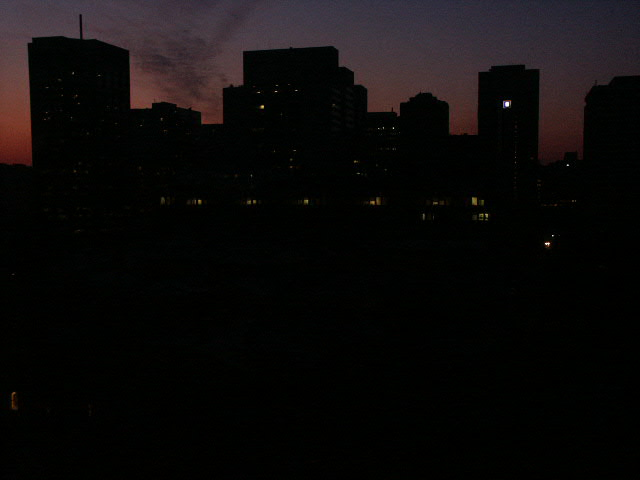
\includegraphics[width=0.75\textwidth]{figures/blackout.jpg}

		\bigskip

		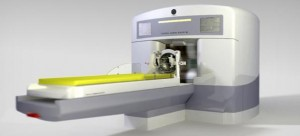
\includegraphics[width=0.75\textwidth]{figures/therac.jpg}
		
		}
		%-%-%-%-%-%-%-%-%-%-%-%-%-%-%-%-%-%-%-%-%-%-%-%-%-%-%-%-%-%
		
	\end{column}

	\begin{column}[c]{0.45 \textwidth}
	
		\medskip
	
		%-%-%-%-%-%-%-%-%-%-%-%-%-%-%-%-%-%-%-%-%-%-%-%-%-%-%-%-%-%
		{
		\centering
		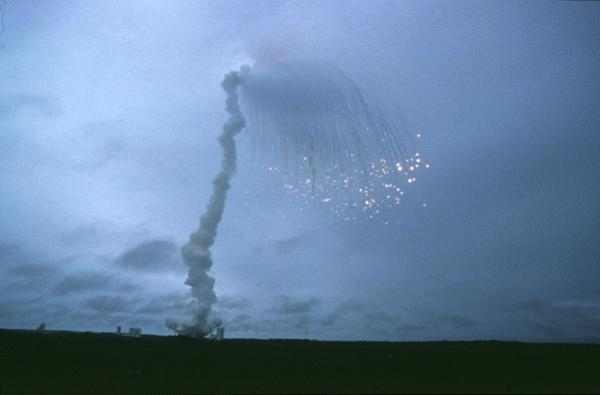
\includegraphics[width=0.65\textwidth]{figures/ariane5.jpg}

		\bigskip

		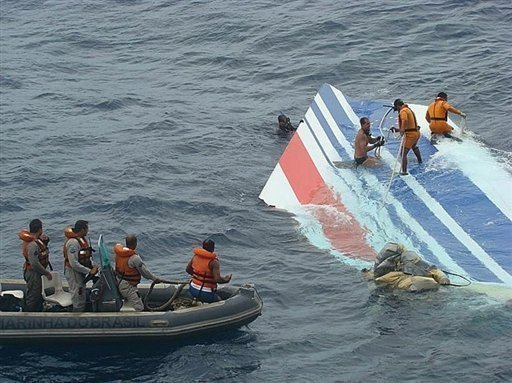
\includegraphics[width=0.65\textwidth]{figures/AF447-crash.jpg}
		
		}
		%-%-%-%-%-%-%-%-%-%-%-%-%-%-%-%-%-%-%-%-%-%-%-%-%-%-%-%-%-%
		
	\end{column}
\end{columns}

\medskip

\begin{itemize}
% 	\item Verification of critical systems
	\item Goal: Ensure safety properties in a \emph{robust} manner
	\begin{itemize}
		\item Properties must hold not only for some timing constants, but also \couleur{around} them
	\end{itemize}
\end{itemize}


\end{frame}


% \begin{frame}
% \frametitle{An example of Scheduling problem}
% \begin{columns}[t] % contents are top vertically aligned
% \begin{column}{5cm} % each column can also be its own environment
% \begin{itemize}
%  \item A processor
%  \item 3 cyclic tasks $\tau_1,\tau_2,\tau_3$
%  \item Each task defined by:
%  \begin{itemize}
%  \item Offset
%  \item Period
%  \item WCET
%  \end{itemize}
% \end{itemize}
% \end{column}
% 
% \begin{column}[T]{5cm} % alternative top-align that's better for graphics Line 13
% \begin{figure}
%  \centering
%  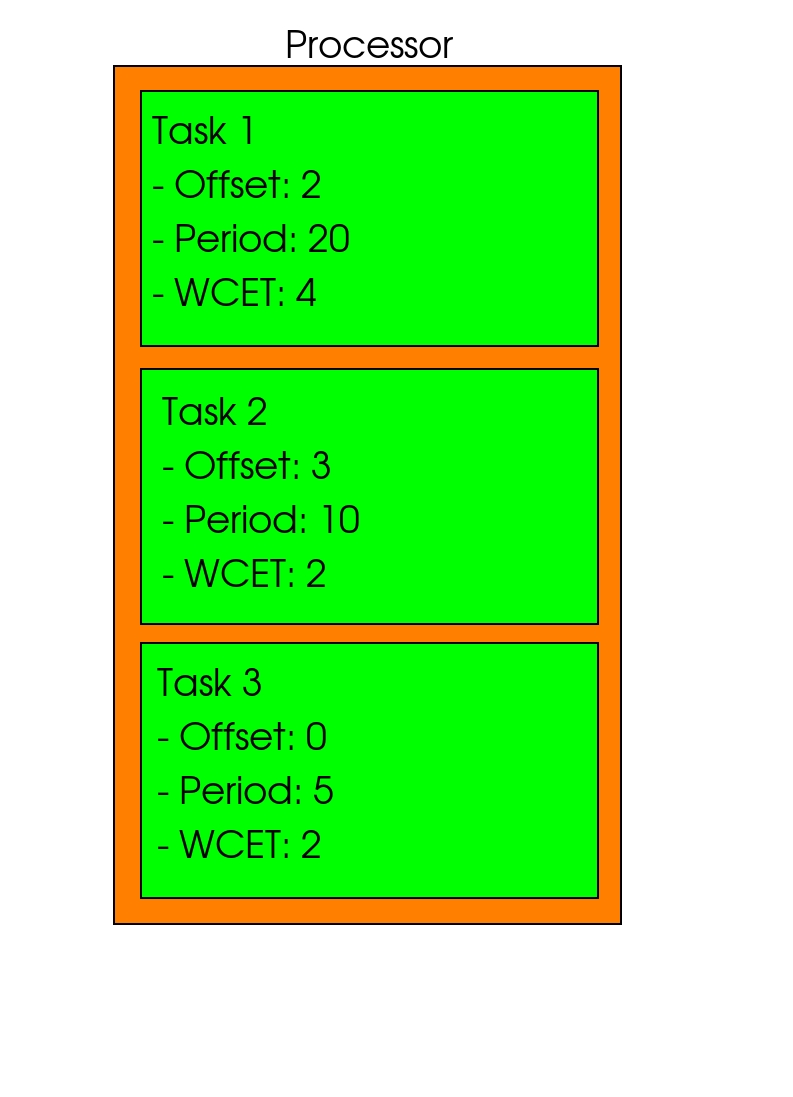
\includegraphics[scale = 0.25]{./figures/proc.jpg}
% \end{figure}
% 
% \end{column}
% \end{columns}
% \end{frame}

%%%%%%%%%%%%%%%%%%%%%%%%%%%%%%%%%%%%%%%%%%%%%%%%%%%%%%%%%%%%%%%%%%%%%%%%%%%%%%%%%%
\begin{frame}
 \frametitle{An Example of a Jobshop Problem}

 \begin{itemize}
	\item A \couleur{job}: a tuple of \couleur{tasks} $((m_1,d_1),\dots,(m_n,d_n))$
	\begin{itemize}
		\item $m_i$: machine to execute the task
		\item $d_i$: duration of this task on this machine
	\end{itemize}
	\item A task can be \couleur{preempted} by another one

	\item For example: $((\textcolor{cpale4}{m_1},3),(\textcolor{cpale7}{m_2},4),(\textcolor{cpale6}{m_3},2))$
\end{itemize}

 \begin{figure}
  \centering
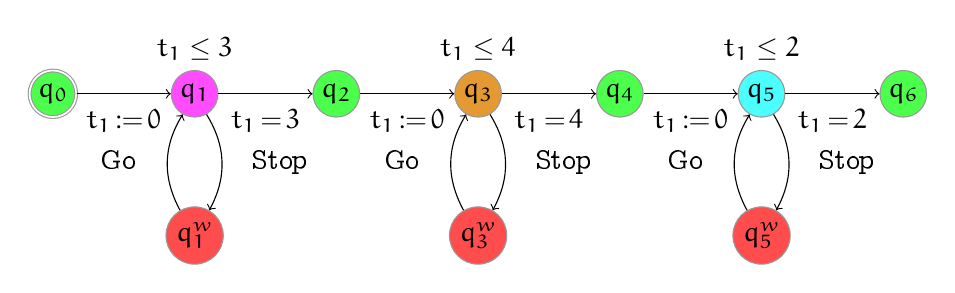
\begin{tikzpicture}[scale=0.6,->, auto]
	\tikzstyle{state}=[circle, minimum size=13pt, inner sep=1.5pt, draw=gris, text=black]

	% ETATS
	\node[state,fill=cpale2, double] (Q0) at (0, 0) {$q_0$};
	\node[state,fill=cpale4] (Q1) at (3, 0) {$q_1$};
	\node[state,fill=cpale2] (Q2) at (6, 0) {$q_2$};
	\node[state,fill=cpale7] (Q3) at (9, 0) {$q_3$};
	\node[state,fill=cpale2] (Q4) at (12,0) {$q_4$};
	\node[state,fill=cpale6] (Q5) at (15,0) {$q_5$};
	\node[state,fill=cpale2] (Q6) at (18,0) {$q_6$};
	\node[state,fill=cpale1] (Q1b) at (3,-3) {$q_{1}^{w}$};
	\node[state,fill=cpale1] (Q3b) at (9,-3) {$q_{3}^{w}$};
	\node[state,fill=cpale1] (Q5b) at (15,-3) {$q_{5}^{w}$}; 

	
	% INVARIANTS
 	\node [above] at (Q1.north) {$t_1 \leq 3$};
 	\node [above] at (Q3.north) {$t_1 \leq 4$};
 	\node [above] at (Q5.north) {$t_1 \leq 2$};

% 	\node [above] at (Q2.north) {$x_2 \leq p_2$};
% 	\node [above] at (Q3.north) {\begin{tabular}{c}  $x_1 \leq p_2$ \\ \end{tabular}};
% 	
 	\path
 		(Q0) edge [below] node {\begin{tabular}{r @{\,} c @{\,} l}
%  			& beginJob1Machine1 & \\
 			$t_1$ & $:=$ & $0$ \\
 		\end{tabular}} (Q1)

 		(Q1) edge [below] node {\begin{tabular}{r @{\,} c @{\,} l}
%  			& beginJob1Machine1 & \\
 			$t_1$ & $=$ & $3$ \\
 		\end{tabular}} (Q2)
 		
		(Q1) edge [bend left, right] node {\begin{tabular}{r @{\,} c @{\,} l}
 			& Stop & \\
%  			$t_1$ & $=$ & $3$ \\
 		\end{tabular}} (Q1b)

		(Q1b) edge [bend left] node {\begin{tabular}{r @{\,} c @{\,} l}
 			& Go & \\
%  			$t_1$ & $=$ & $3$ \\
 		\end{tabular}} (Q1)

 		(Q2) edge [below] node {\begin{tabular}{r @{\,} c @{\,} l}
%  			& beginJob1Machine1 & \\
 			$t_1$ & $:=$ & $0$ \\
 		\end{tabular}} (Q3)

 		(Q3) edge [below] node {\begin{tabular}{r @{\,} c @{\,} l}
%  			& beginJob1Machine1 & \\
 			$t_1$ & $=$ & $4$ \\
 		\end{tabular}} (Q4)

		(Q3) edge [bend left, right] node {\begin{tabular}{r @{\,} c @{\,} l}
 			& Stop & \\
%  			$t_1$ & $=$ & $3$ \\
 		\end{tabular}} (Q3b)

		(Q3b) edge [bend left] node {\begin{tabular}{r @{\,} c @{\,} l}
 			& Go & \\
%  			$t_1$ & $=$ & $3$ \\
 		\end{tabular}} (Q3)

 		(Q4) edge [below] node {\begin{tabular}{r @{\,} c @{\,} l}
%  			& beginJob1Machine1 & \\
 			$t_1$ & $:=$ & $0$ \\
 		\end{tabular}} (Q5)

 		(Q5) edge [below] node {\begin{tabular}{r @{\,} c @{\,} l}
%  			& beginJob1Machine1 & \\
 			$t_1$ & $=$ & $2$ \\
 		\end{tabular}} (Q6)

		(Q5) edge [bend left, right] node {\begin{tabular}{r @{\,} c @{\,} l}
 			& Stop & \\
%  			$t_1$ & $=$ & $3$ \\
 		\end{tabular}} (Q5b)

		(Q5b) edge [bend left] node {\begin{tabular}{r @{\,} c @{\,} l}
 			& Go & \\
%  			$t_1$ & $=$ & $3$ \\
 		\end{tabular}} (Q5)

% 		(Q0) edge [above] node {\begin{tabular}{r @{\,} c @{\,} l}
% 			$x_1$ & $\geq$ & $p_2$ \\
% 			& $c$ & \\
% 		\end{tabular}} (Q4)
% % 
% 		(Q1) edge [] node {$a$} (Q2)
% 		(Q1) edge [below left] node {\begin{tabular}{r @{\,} c @{\,} l}
% 			$x_1$ & $\geq$ & $3$ \\
% 			& $b$ & \\
% 		\end{tabular}} (Q3)
% 
% 		(Q2) edge [loop right] node {\begin{tabular}{r @{\,} c @{\,} l}
% 			$x_1$ & $\geq$ & $p_1$ \\
% 			& $a$ & \\
% 			$x_1$ & $:=$ & $0$ \\
% 		\end{tabular}} (Q2)
% 
% 		(Q3) edge [loop right] node {$b$} (Q3)
% 
% 		(Q4) edge [loop right] node {$c$} (Q4)
	;
\end{tikzpicture}
 \end{figure}

\end{frame}
%%%%%%%%%%%%%%%%%%%%%%%%%%%%%%%%%%%%%%%%%%%%%%%%%%%%%%%%%%%%%%%%%%%%%%%%%%%%%%%%%


%%%%%%%%%%%%%%%%%%%%%%%%%%%%%%%%%%%%%%%%%%%%%%%%%%%%%%%%%%%%%%%%%%%%%%%%%%%%%%%%%%
\begin{frame}
 \frametitle{The Jobshop Problem}

 
\begin{jobshopproblem}
	Given a set of jobs $J_1,\dots,J_m$
% 	Given a set of tasts $\tau_1,\dots,\tau_n$
 
	Given a deadline $d$
 
% 	Question: \couleur{Is the system schedulable on one processor?}
	Question: \couleur{Can all the jobs be completed within $d$ time units?}
\end{jobshopproblem}

\pause

\begin{itemize}
	\item Use of \couleur{timed automata}
	
	\bigskip
	
	\item Timed model checking techniques give the answer: \couleur{yes/no}
\end{itemize}

\end{frame}

% \begin{frame}
%  \frametitle{An Example of a Jobshop Problem with Preemption}
%  \begin{figure}
%   \centering
%   \begin{tikzpicture}
%    
%   \end{tikzpicture}
% 
%  \end{figure}
% 
% \end{frame}
%%%%%%%%%%%%%%%%%%%%%%%%%%%%%%%%%%%%%%%%%%%%%%%%%%%%%%%%%%%%%%%%%%%%%%%%%%%%%%%%%%

%%%%%%%%%%%%%%%%%%%%%%%%%%%%%%%%%%%%%%%%%%%%%%%%%%%%%%%%%%%%%%%%%%%%%%%%%%%%%%%%%%
\begin{frame}
\frametitle{Synthesis of Parameters}

\begin{itemize}
	\item More difficult problem: \couleur{find values of the durations} for which the jobshop is schedulable in a given deadline

	\bigskip

	\item Idea: reason with unknown constants or \couleur{parameters}
	\begin{itemize}
		\item Use of \couleur{parametric timed automata} (PTAs) equipped with stopwatches
	\end{itemize}

	
	\bigskip

	\item Interesting applications
	\begin{itemize}
		\item Ensure the \couleur{robustness} of the system
		\item Allow the designer to \couleur{optimize} timing delays
	\end{itemize}

	
	\bigskip


	\item Difficult problem
	\begin{itemize}
		\item Both concurrent behavior and timed behavior
		\item Undecidable in general
	\end{itemize}

\end{itemize}

\end{frame}

% \begin{frame}
% \frametitle{An example of Scheduling problem}
% \begin{columns}[t] % contents are top vertically aligned
% \begin{column}{5cm} % each column can also be its own environment
% \begin{itemize}
%  \item A processor
%  \item 3 cyclic tasks $\tau_1,\tau_2,\tau_3$
%  \item Each task defined by:
%  \begin{itemize}
%  \item Offset
%  \item Period
%  \item WCET
%  \end{itemize}
% \end{itemize}
% \end{column}
% 
% \begin{column}[T]{5cm} % alternative top-align that's better for graphics Line 13
% \begin{figure}
%  \centering
%  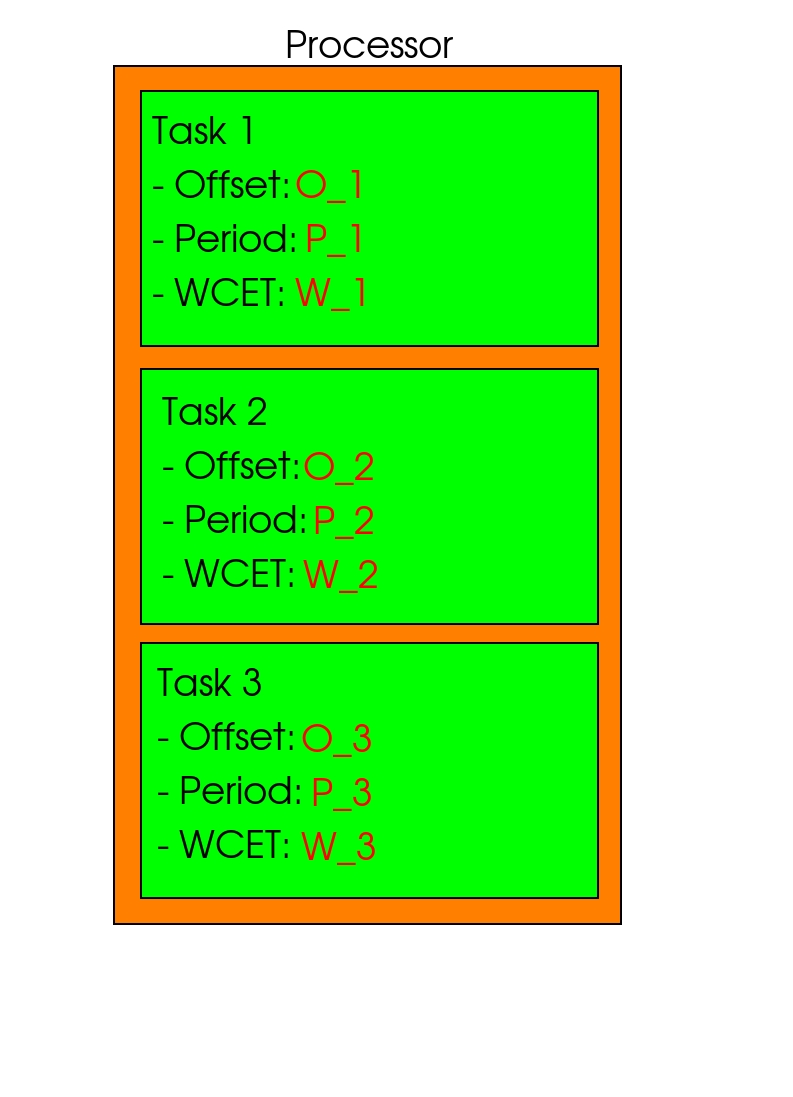
\includegraphics[scale = 0.25]{./figures/proc2.jpg}
% \end{figure}
% 
% \end{column}
% \end{columns}
% \end{frame}


\begin{frame}
 \frametitle{An Example of a Parametric Jobshop Problem}
\begin{itemize}
 \item A job: a tuple $((m_1,d_1),\dots,(m_n,d_n))$
 \item For example: $((\textcolor{cpale4}{m_1},\coulparam{d_1}),(\textcolor{cpale7}{m_2},\coulparam{d_2}),(\textcolor{cpale6}{m_3},\coulparam{d_3}))$
\end{itemize}
 \begin{figure}
  \centering
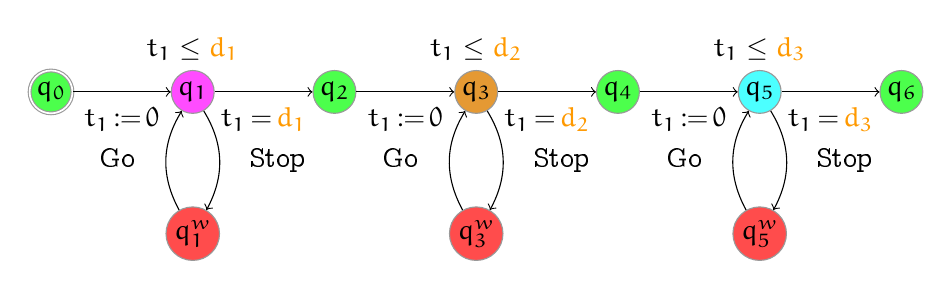
\begin{tikzpicture}[scale=0.6,->, auto]
	\tikzstyle{state}=[circle, minimum size=13pt, inner sep=1pt, draw=gris, text=black]

	% ETATS
	\node[state,fill=cpale2, double] (Q0) at (0, 0) {$q_0$};
	\node[state,fill=cpale4] (Q1) at (3, 0) {$q_1$};
	\node[state,fill=cpale2] (Q2) at (6, 0) {$q_2$};
	\node[state,fill=cpale7] (Q3) at (9, 0) {$q_3$};
	\node[state,fill=cpale2] (Q4) at (12,0) {$q_4$};
	\node[state,fill=cpale6] (Q5) at (15,0) {$q_5$};
	\node[state,fill=cpale2] (Q6) at (18,0) {$q_6$};
	\node[state,fill=cpale1] (Q1b) at (3,-3) {$q_{1}^{w}$};
	\node[state,fill=cpale1] (Q3b) at (9,-3) {$q_{3}^{w}$};
	\node[state,fill=cpale1] (Q5b) at (15,-3) {$q_{5}^{w}$}; 

	
	% INVARIANTS
 	\node [above] at (Q1.north) {$t_1 \leq \coulparam{d_1}$};
 	\node [above] at (Q3.north) {$t_1 \leq \coulparam{d_2}$};
 	\node [above] at (Q5.north) {$t_1 \leq \coulparam{d_3}$};

% 	\node [above] at (Q2.north) {$x_2 \leq p_2$};
% 	\node [above] at (Q3.north) {\begin{tabular}{c}  $x_1 \leq p_2$ \\ \end{tabular}};
% 	
 	\path
 		(Q0) edge [below] node {\begin{tabular}{r @{\,} c @{\,} l}
%  			& beginJob1Machine1 & \\
 			$t_1$ & $:=$ & $0$ \\
 		\end{tabular}} (Q1)

 		(Q1) edge [below] node {\begin{tabular}{r @{\,} c @{\,} l}
%  			& beginJob1Machine1 & \\
 			$t_1$ & $=$ & $\coulparam{d_1}$ \\
 		\end{tabular}} (Q2)
 		
		(Q1) edge [bend left, right] node {\begin{tabular}{r @{\,} c @{\,} l}
 			& Stop & \\
%  			$t_1$ & $=$ & $3$ \\
 		\end{tabular}} (Q1b)

		(Q1b) edge [bend left] node {\begin{tabular}{r @{\,} c @{\,} l}
 			& Go & \\
%  			$t_1$ & $=$ & $3$ \\
 		\end{tabular}} (Q1)

 		(Q2) edge [below] node {\begin{tabular}{r @{\,} c @{\,} l}
%  			& beginJob1Machine1 & \\
 			$t_1$ & $:=$ & $0$ \\
 		\end{tabular}} (Q3)

 		(Q3) edge [below] node {\begin{tabular}{r @{\,} c @{\,} l}
%  			& beginJob1Machine1 & \\
 			$t_1$ & $=$ & $\coulparam{d_2}$ \\
 		\end{tabular}} (Q4)

		(Q3) edge [bend left, right] node {\begin{tabular}{r @{\,} c @{\,} l}
 			& Stop & \\
%  			$t_1$ & $=$ & $3$ \\
 		\end{tabular}} (Q3b)

		(Q3b) edge [bend left] node {\begin{tabular}{r @{\,} c @{\,} l}
 			& Go & \\
%  			$t_1$ & $=$ & $3$ \\
 		\end{tabular}} (Q3)

 		(Q4) edge [below] node {\begin{tabular}{r @{\,} c @{\,} l}
%  			& beginJob1Machine1 & \\
 			$t_1$ & $:=$ & $0$ \\
 		\end{tabular}} (Q5)

 		(Q5) edge [below] node {\begin{tabular}{r @{\,} c @{\,} l}
%  			& beginJob1Machine1 & \\
 			$t_1$ & $=$ & $\coulparam{d_3}$ \\
 		\end{tabular}} (Q6)

		(Q5) edge [bend left, right] node {\begin{tabular}{r @{\,} c @{\,} l}
 			& Stop & \\
%  			$t_1$ & $=$ & $3$ \\
 		\end{tabular}} (Q5b)

		(Q5b) edge [bend left] node {\begin{tabular}{r @{\,} c @{\,} l}
 			& Go & \\
%  			$t_1$ & $=$ & $3$ \\
 		\end{tabular}} (Q5)

% 		(Q0) edge [above] node {\begin{tabular}{r @{\,} c @{\,} l}
% 			$x_1$ & $\geq$ & $p_2$ \\
% 			& $c$ & \\
% 		\end{tabular}} (Q4)
% % 
% 		(Q1) edge [] node {$a$} (Q2)
% 		(Q1) edge [below left] node {\begin{tabular}{r @{\,} c @{\,} l}
% 			$x_1$ & $\geq$ & $3$ \\
% 			& $b$ & \\
% 		\end{tabular}} (Q3)
% 
% 		(Q2) edge [loop right] node {\begin{tabular}{r @{\,} c @{\,} l}
% 			$x_1$ & $\geq$ & $p_1$ \\
% 			& $a$ & \\
% 			$x_1$ & $:=$ & $0$ \\
% 		\end{tabular}} (Q2)
% 
% 		(Q3) edge [loop right] node {$b$} (Q3)
% 
% 		(Q4) edge [loop right] node {$c$} (Q4)
	;
\end{tikzpicture}
 \end{figure}
\begin{itemize}
\item For which value of $(\coulparam{d_1},\coulparam{d_2},\coulparam{d_3})$ is the system schedulable in $d$ time units?
\end{itemize}
\end{frame}
%%%%%%%%%%%%%%%%%%%%%%%%%%%%%%%%%%%%%%%%%%%%%%%%%%%%%%%%%%%%%%%%%%%%%%%%%%%%%%%%%%


%%%%%%%%%%%%%%%%%%%%%%%%%%%%%%%%%%%%%%%%%%%%%%%%%%%%%%%%%%%%%%%%%%%%%%%%%%%%%%%%%
\begin{frame}
\frametitle{Problems}

% We consider a system modeled by a parametric timed automaton. %~$\A$.

\begin{itemize}
	\item \couleur{The good parameters problem}
	
	\begin{itemize}
		\item ``Given a \couleur{bounded parameter domain} $\Vo$, find a set of parameter valuations of \couleur{good} behavior in~$\Vo$'' % (ideally the largest one)
	\end{itemize}
	

	% %-%-%-%-%-%-%-%-%-%-%-%-%-%-%-%-%-%-%-%-%-%-%-%-%-%-%-%-%-%-%
	\begin{figure}
	{

	\centering
	\footnotesize

	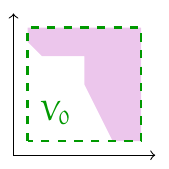
\begin{tikzpicture}[scale=0.18]

% 		\path[use as bounding box] (-1,-1) rectangle (1,1);
		\path[use as bounding box] (-4, -4) rectangle (4, 4);
		\draw<2->[fill=outputcolor!25, draw=none]
			(2, -4) -- (0, 0) -- (0, 2) -- (-3, 2) -- (-4, 3) -- (-4, 4) -- (4, 4) -- (4, -4) -- cycle;

% 		\node<2-> (k) at (2, 2) [text=outputcolor] {\large{$\Ko$}};

		% VO
		\tikzstyle{v0} = [line width=1pt, draw=inputcolor, dashed]
		\path[v0] (-4, -4) -- (-4, 4) -- (4, 4) -- (4, -4) -- cycle;
		\node (v0) at (-2, -2) [text=inputcolor] {$\Vo$};

		\draw[->] (-5, -5) -- (-5, 5);
		\draw[->] (-5, -5) -- (5, -5);
		

	\end{tikzpicture}

	}
	\end{figure}
	% %-%-%-%-%-%-%-%-%-%-%-%-%-%-%-%-%-%-%-%-%-%-%-%-%-%-%-%-%-%-%
	
% 	\bigskip

	\item<3-> The \couleur{inverse problem}: A simpler problem
	\begin{itemize}
		\item ``Given a \couleur{reference parameter valuation} $\pio$, find other valuations around $\pio$ of \couleur{same} behavior''
	\end{itemize}
	
	% %-%-%-%-%-%-%-%-%-%-%-%-%-%-%-%-%-%-%-%-%-%-%-%-%-%-%-%-%-%-%
	\begin{figure}
	{

	\centering
	\footnotesize

	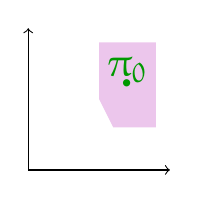
\begin{tikzpicture}[scale=0.18]

		\draw[->] (-5, -5) -- (-5, 5);
		\draw[->] (-5, -5) -- (5, -5);
		
		\path[use as bounding box] (-1,-1) rectangle (1,1);
% 		\draw<4->[fill=outputcolor!25, draw=none]
% 			(-3, -3) -- (-4, 3) -- (-2, 4) -- (3, 3) -- (5, 0) -- (3, -4) -- cycle;
		\draw<4->[fill=outputcolor!25, draw=none]
			(1, -2) -- (0, 0) -- (0, 4) -- (4, 4) -- (4, -2) -- cycle;

% 		\node<4-> (k) at (-1,-2) {\large{$\Ko$}};
		\node (point) at (2, 1) {\Huge{$\coulinput{\cdot}$}};
		\node (pi) at (2, 2) {\Large{$\pio$}};

	\end{tikzpicture}

	}
	\end{figure}
	% %-%-%-%-%-%-%-%-%-%-%-%-%-%-%-%-%-%-%-%-%-%-%-%-%-%-%-%-%-%-%

\end{itemize}

\end{frame}
%%%%%%%%%%%%%%%%%%%%%%%%%%%%%%%%%%%%%%%%%%%%%%%%%%%%%%%%%%%%%%%%%%%%%%%%%%%%%%%%%%

%%%%%%%%%%%%%%%%%%%%%%%%%%%%%%%%%%%%%%%%%%%%%%%%%%%%%%%%%%%%%%%%%%%%%%%%%%%%%%%%%%%
% Plan
\begin{frame}
	\frametitle{\plan{}}
	\tableofcontents[hideallsubsections]
\end{frame}
%%%%%%%%%%%%%%%%%%%%%%%%%%%%%%%%%%%%%%%%%%%%%%%%%%%%%%%%%%%%%%%%%%%%%%%%%%%%%%%%%%


%%%%%%%%%%%%%%%%%%%%%%%%%%%%%%%%%%%%%%%%%%%%%%%%%%%%%%%%%%%%%%%%%%%%%%%%%%%%%%%%%%
%%%%%%%%%%%%%%%%%%%%%%%%%%%%%%%%%%%%%%%%%%%%%%%%%%%%%%%%%%%%%%%%%%%%%%%%%%%%%%%%%%
\section{The Inverse Method}
%%%%%%%%%%%%%%%%%%%%%%%%%%%%%%%%%%%%%%%%%%%%%%%%%%%%%%%%%%%%%%%%%%%%%%%%%%%%%%%%%%
%%%%%%%%%%%%%%%%%%%%%%%%%%%%%%%%%%%%%%%%%%%%%%%%%%%%%%%%%%%%%%%%%%%%%%%%%%%%%%%%%%


%%%%%%%%%%%%%%%%%%%%%%%%%%%%%%%%%%%%%%%%%%%%%%%%%%%%%%%%%%%%%%%%%%%%%%%%%%%%%%%%%%%
% Plan
\begin{frame}
	\frametitle{\plan{}}
	\tableofcontents[currentsection, hideallsubsections]
\end{frame}
%%%%%%%%%%%%%%%%%%%%%%%%%%%%%%%%%%%%%%%%%%%%%%%%%%%%%%%%%%%%%%%%%%%%%%%%%%%%%%%%%%


%%%%%%%%%%%%%%%%%%%%%%%%%%%%%%%%%%%%%%%%%%%%%%%%%%%%%%%%%%%%%%%%%%%%%%%%%%%%%%%%%%

%%%%%%%%%%%%%%%%%%%%%%%%%%%%%%%%%%%%%%%%%%%%%%%%%%%%%%%%%%%%%%%%%%%%%%%%%%%%%%%%%%





%%%%%%%%%%%%%%%%%%%%%%%%%%%%%%%%%%%%%%%%%%%%%%%%%%%%%%%%%%%%%%%%%%%%%%%%%%%%%%%%%%
\begin{frame}
\frametitle{Trace Set}

\begin{itemize}
	\item \couleur{Trace}: A time-abstract run
\end{itemize}
{
\centering
\footnotesize

\begin{tikzpicture}[scale=0.2, ->, >=stealth', shorten >=2pt, auto, thin]
\tikzstyle{state}=[circle, minimum size=12pt, draw=none, text=black, shade=ball, inner sep=3pt]

% 	\node[state,ball color=cv1] (I1I1) at (0

	\node[state, ball color=cv1]         (Q0) at (0,4) {};
	\node[state, ball color=cv2]         (Q1) at (5,4) {};
	\node[state, ball color=cv3]         (Q2) at (10,4) {};
	\node[state, ball color=cv4]         (Q3) at (15,4) {};
	\node[state, ball color=cv5]         (Q5) at (20,4) {};
	\node[state, ball color=cv7]         (Q8) at (25,4) {};
	\node[state, ball color=cv6]         (Q9) at (30,4) {};
	\node[state, ball color=cv8]        (Q13) at (35,4) {};
	\node[state, ball color=cv10]        (Q14) at (40,4) {};
	\node[state, ball color=cv9]        (Q15) at (45,4) {};
	\node[state, ball color=cv11]        (Q19) at (50,4) {};

	\path
		(Q0) edge [double] node {$\coulact{J_{1,m1}^\uparrow}$} (Q1)
		(Q1) edge [double] node {$\coulact{J_{2,m2}^\uparrow}$} (Q2)
		(Q2) edge [double] node {$\coulact{J_{1,m1}^\downarrow}$} (Q3)
		(Q3) edge [double] node {$\coulact{J_{2,m2}^{h}}$} (Q5)
		(Q5) edge [double] node {$\coulact{J_{1,m2}^\uparrow}$} (Q8)
		(Q8) edge [double] node {$\coulact{J_{1,m2}^\downarrow}$} (Q9)
		(Q9) edge [double] node {$\coulact{J_{2,m2}^{r}}$} (Q13)
		(Q13) edge [double] node {$\coulact{J_{1,m3}^\uparrow}$} (Q14)
		(Q14) edge [double] node {$\coulact{J_{2,m2}^\downarrow}$} (Q15)
		(Q15) edge [double] node {$\coulact{J_{1,m3}^\uparrow}$} (Q19)
		;

\end{tikzpicture}

}
\begin{itemize}
	\item \couleur{Trace set}: set of all traces of a PTA

	\bigskip

	\item Graphical representation under the form of a \couleur{tree}
	
	\begin{itemize}
		\item Does not give any information on the \couleur{branching behavior} though

% 		\medskip
% 
% 		\item Example of trace set for the jobshop example
	\end{itemize}

%-%-%-%-%-%-%-%-%-%-%-%-%-%-%-%-%-%-%-%-%-%-%-%-%-%-%-%-%-%-%

%-%-%-%-%-%-%-%-%-%-%-%-%-%-%-%-%-%-%-%-%-%-%-%-%-%-%-%-%-%-%



\end{itemize}

\end{frame}
%%%%%%%%%%%%%%%%%%%%%%%%%%%%%%%%%%%%%%%%%%%%%%%%%%%%%%%%%%%%%%%%%%%%%%%%%%%%%%%%%%

%%%%%%%%%%%%%%%%%%%%%%%%%%%%%%%%%%%%%%%%%%%%%%%%%%%%%%%%%%%%%%%%%%%%%%%%%%%%%%%%%%
\begin{frame}
\frametitle{The Inverse Method}

\begin{itemize}

	\item \coulinput{Input}
	\begin{itemize}
		\item $\A$: A PTA equipped with stopwatches
		\item $\pio$: A \couleur{reference valuation} of all the parameters of $\A$
% 		\begin{itemize}
%  			\item Exemplifying a good behavior\\
% 			(all traces of \symb{$\A[\pio]$} correspond to good behaviors)
% 		\end{itemize}
	\end{itemize}

	\bigskip

	\item<2-> \couloutput{Output: tile $\Ko$}
	\begin{itemize}
		\item Convex \couleur{constraint} on the parameters such that
		\begin{itemize}
			\item $\pio \models \Ko$
			\item For all points $\pi \models \Ko$, $\A[\pi]$ and $\A[\pio]$ have the \couleur{same trace sets}
		\end{itemize}
	\end{itemize}
\end{itemize}

\bigskip

% %-%-%-%-%-%-%-%-%-%-%-%-%-%-%-%-%-%-%-%-%-%-%-%-%-%-%-%-%-%-%
\begin{figure}
{

\centering
\footnotesize

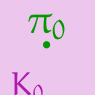
\begin{tikzpicture}[scale=0.25]

	\path[use as bounding box] (-1,-1) rectangle (1,1);
%     \node<2-> (patate) at (0,0) [regular polygon, regular polygon sides=5, minimum height=6em, fill=outputcolor!25] {};
%     \node (patate) at (0,0) [regular polygon, regular polygon sides=5, minimum height=6em, ] {};
	\draw<2->[fill=outputcolor!25, draw=none]
		(-3, -3) -- (-4, 3) -- (-2, 4) -- (3, 3) -- (5, 0) -- (3, -4) -- cycle;

	\node<2-> (k) at (-1,-2) {\large{$\Ko$}};
	\node (point) at (0,0) {\Huge{$\coulinput{\cdot}$}};
	\node (pi) at (0,1) {\Large{$\pio$}};

\end{tikzpicture}

}
\end{figure}
% %-%-%-%-%-%-%-%-%-%-%-%-%-%-%-%-%-%-%-%-%-%-%-%-%-%-%-%-%-%-%

\end{frame}
%%%%%%%%%%%%%%%%%%%%%%%%%%%%%%%%%%%%%%%%%%%%%%%%%%%%%%%%%%%%%%%%%%%%%%%%%%%%%%%%%%





%%%%%%%%%%%%%%%%%%%%%%%%%%%%%%%%%%%%%%%%%%%%%%%%%%%%%%%%%%%%%%%%%%%%%%%%%%%%%%%%%%
\begin{frame}
\frametitle{The Inverse Method: General Idea}

\begin{itemize}
	\item The idea \refer{ACEF09}
	\begin{itemize}
		\item Instead of negating bad states (as in ``CEGAR'' approaches), we remove \couleur{$\pio$-incompatible} states
	\end{itemize}
\end{itemize}


%-%-%-%-%-%-%-%-%-%-%-%-%-%-%-%-%-%-%-%-%-%-%-%-%-%-%-%-%-%-%
{
\centering
\footnotesize

\begin{tikzpicture}[>=stealth', node distance=3cm, semithick]
	\tikzstyle{state} = [circle, minimum size=12pt, draw=none, shade=ball, inner sep=1.5pt]
	\tikzstyle{contrainte}=[rectangle, draw=couleurgood, inner sep=1pt, text width=2cm, font=\scriptsize]
	\tikzstyle{transition} = [->, double]
	\tikzstyle{liaison} = [-, dashed]
	\tikzstyle{croix} = [thick, draw=couleurbad]

	\path[use as bounding box] (-1, -0.5) rectangle (7, 3);

	% ETATS
	\node[state, ball color=cv1] at (0, 0) (Q0) {};
	\node[state, ball color=cv2] at (2.5, 0) (Q1) {};
	\node[state, ball color=cv3] at (5, 0) (Q2) {};
	\node[state, ball color=cv4] at (5, 1) (Q3) {};

	% CONTRAINTES
	\node[contrainte, fill=cv1!30] at (0, -1) (C0) {\centering \begin{tabular}{r @{\,} c @{\,} l }
		$\coulparam{d_1}$ & $\leq$ & $\coulparam{d_2}$ \\
		& & \\
	\end{tabular}
	
	};

	\node[contrainte, fill=cv2!30] at (2.5, -1) (C1) {\centering \begin{tabular}{r @{\,} c @{\,} l }
		$\coulparam{d_1}$ & $\leq$ & $\coulparam{d_2}$ \\
		$\coulparam{d_1}$ & $\leq$ & $\coulparam{d_3} + \coulparam{d_4}$ \\
	\end{tabular}
	};

	\node[contrainte, fill=cv3!30] at (5, -1) (C2) {\centering \begin{tabular}{r @{\,} c @{\,} l }
		$\coulparam{d_1}$ & $\leq$ & $\coulparam{d_2}$ \\
		$\coulparam{d_1}$ & $\leq$ & $\coulparam{d_3} + \coulparam{d_4}$ \\
		$\coulparam{d_3}$ & $\geq$ & $\coulparam{d_4}$ \\
	\end{tabular}	
	};

	\node[contrainte, fill=cv4!30, draw=couleurbad] at (5, 2) (C3) {\centering \begin{tabular}{r @{\,} c @{\,} l }
		$\coulparam{d_1}$ & $\leq$ & $\coulparam{d_2}$ \\
		$\coulparam{d_1}$ & $\leq$ & $\coulparam{d_3} + \coulparam{d_4}$ \\
		$\textcolor{red}{d_3}$ & $\textcolor{red}{<}$ & $\textcolor{red}{d_4}$ \\
	\end{tabular}	
	};


	% TRANSITIONS
	\path (Q0) edge [transition, above] node {$\coulact{a}$} (Q1);
	\path (Q1) edge [transition, above] node {$\coulact{b}$} (Q2);
	\path (Q1) edge [transition, above] node {$\coulact{c}$} (Q3);

	% LIAISONS
	\path (Q0) edge [liaison] (C0);
	\path (Q1) edge [liaison] (C1);
	\path (Q2) edge [liaison] (C2);
	\path (Q3) edge [liaison] (C3);
	
	% CROIX
% 	\path (4, 3) edge [croix] (6, 1);
% 	\path (4, 1) edge [croix] (6, 3);
	\path<2-> (3.5, 3) edge [croix] (6.5, 0.5);
	\path<2-> (3.5, 0.5) edge [croix] (6.5, 3);


\end{tikzpicture}

}
%-%-%-%-%-%-%-%-%-%-%-%-%-%-%-%-%-%-%-%-%-%-%-%-%-%-%-%-%-%-%



\end{frame}
%%%%%%%%%%%%%%%%%%%%%%%%%%%%%%%%%%%%%%%%%%%%%%%%%%%%%%%%%%%%%%%%%%%%%%%%%%%%%%%%%%


% 
% 
% %%%%%%%%%%%%%%%%%%%%%%%%%%%%%%%%%%%%%%%%%%%%%%%%%%%%%%%%%%%%%%%%%%%%%%%%%%%%%%%%%
% \begin{frame}
% \frametitle{Application to the Jobshop Example}
% \end{frame}
% %%%%%%%%%%%%%%%%%%%%%%%%%%%%%%%%%%%%%%%%%%%%%%%%%%%%%%%%%%%%%%%%%%%%%%%%%%%%%%%%%


% %%%%%%%%%%%%%%%%%%%%%%%%%%%%%%%%%%%%%%%%%%%%%%%%%%%%%%%%%%%%%%%%%%%%%%%%%%%%%%%%%
% %%%%%%%%%%%%%%%%%%%%%%%%%%%%%%%%%%%%%%%%%%%%%%%%%%%%%%%%%%%%%%%%%%%%%%%%%%%%%%%%%
% \section{State Merging}
% %%%%%%%%%%%%%%%%%%%%%%%%%%%%%%%%%%%%%%%%%%%%%%%%%%%%%%%%%%%%%%%%%%%%%%%%%%%%%%%%%
% %%%%%%%%%%%%%%%%%%%%%%%%%%%%%%%%%%%%%%%%%%%%%%%%%%%%%%%%%%%%%%%%%%%%%%%%%%%%%%%%%
% 
% 
% %%%%%%%%%%%%%%%%%%%%%%%%%%%%%%%%%%%%%%%%%%%%%%%%%%%%%%%%%%%%%%%%%%%%%%%%%%%%%%%%%%%
% % Plan
% \begin{frame}
% 	\frametitle{\plan{}}
% 	\tableofcontents[currentsection, hideallsubsections]
% \end{frame}
% %%%%%%%%%%%%%%%%%%%%%%%%%%%%%%%%%%%%%%%%%%%%%%%%%%%%%%%%%%%%%%%%%%%%%%%%%%%%%%%%%%
% 
% 
% 
% 
% %%%%%%%%%%%%%%%%%%%%%%%%%%%%%%%%%%%%%%%%%%%%%%%%%%%%%%%%%%%%%%%%%%%%%%%%%%%%%%%%%
% \begin{frame}
%  \frametitle{Principle}
% \end{frame}
% %%%%%%%%%%%%%%%%%%%%%%%%%%%%%%%%%%%%%%%%%%%%%%%%%%%%%%%%%%%%%%%%%%%%%%%%%%%%%%%%%
% \begin{itemize}
%  \item Let $s$ and $s'$ be two states sharing the same location
%  \item Under certain circonstances 
% \end{itemize}
% 
% 
% 
% 
% 
% %%%%%%%%%%%%%%%%%%%%%%%%%%%%%%%%%%%%%%%%%%%%%%%%%%%%%%%%%%%%%%%%%%%%%%%%%%%%%%%%%
% \begin{frame}
%  \frametitle{Application to the Jobshop Problem}
% \end{frame}
% %%%%%%%%%%%%%%%%%%%%%%%%%%%%%%%%%%%%%%%%%%%%%%%%%%%%%%%%%%%%%%%%%%%%%%%%%%%%%%%%%
% 
% % %%%%%%%%%%%%%%%%%%%%%%%%%%%%%%%%%%%%%%%%%%%%%%%%%%%%%%%%%%%%%%%%%%%%%%%%%%%%%%%%%
% % \begin{frame}
% %  \frametitle{Theoretical Results}
% % \end{frame}
% % %%%%%%%%%%%%%%%%%%%%%%%%%%%%%%%%%%%%%%%%%%%%%%%%%%%%%%%%%%%%%%%%%%%%%%%%%%%%%%%%%

% 
% %%%%%%%%%%%%%%%%%%%%%%%%%%%%%%%%%%%%%%%%%%%%%%%%%%%%%%%%%%%%%%%%%%%%%%%%%%%%%%%%%
% %%%%%%%%%%%%%%%%%%%%%%%%%%%%%%%%%%%%%%%%%%%%%%%%%%%%%%%%%%%%%%%%%%%%%%%%%%%%%%%%%
% \section{Experiments}
% %%%%%%%%%%%%%%%%%%%%%%%%%%%%%%%%%%%%%%%%%%%%%%%%%%%%%%%%%%%%%%%%%%%%%%%%%%%%%%%%%
% %%%%%%%%%%%%%%%%%%%%%%%%%%%%%%%%%%%%%%%%%%%%%%%%%%%%%%%%%%%%%%%%%%%%%%%%%%%%%%%%%
% 
% 
% %%%%%%%%%%%%%%%%%%%%%%%%%%%%%%%%%%%%%%%%%%%%%%%%%%%%%%%%%%%%%%%%%%%%%%%%%%%%%%%%%%%
% % Plan
% \begin{frame}
% 	\frametitle{\plan{}}
% 	\tableofcontents[currentsection, hideallsubsections]
% \end{frame}
% %%%%%%%%%%%%%%%%%%%%%%%%%%%%%%%%%%%%%%%%%%%%%%%%%%%%%%%%%%%%%%%%%%%%%%%%%%%%%%%%%%
% 
% 
% 
% %%%%%%%%%%%%%%%%%%%%%%%%%%%%%%%%%%%%%%%%%%%%%%%%%%%%%%%%%%%%%%%%%%%%%%%%%%%%%%%%%
% \begin{frame}
%  \frametitle{Experimentations}
% \end{frame}
% %%%%%%%%%%%%%%%%%%%%%%%%%%%%%%%%%%%%%%%%%%%%%%%%%%%%%%%%%%%%%%%%%%%%%%%%%%%%%%%%%
% 
% 
% 
% 



%%%%%%%%%%%%%%%%%%%%%%%%%%%%%%%%%%%%%%%%%%%%%%%%%%%%%%%%%%%%%%%%%%%%%%%%%%%%%%%%%
%%%%%%%%%%%%%%%%%%%%%%%%%%%%%%%%%%%%%%%%%%%%%%%%%%%%%%%%%%%%%%%%%%%%%%%%%%%%%%%%%
\section{Implementation}
%%%%%%%%%%%%%%%%%%%%%%%%%%%%%%%%%%%%%%%%%%%%%%%%%%%%%%%%%%%%%%%%%%%%%%%%%%%%%%%%%
%%%%%%%%%%%%%%%%%%%%%%%%%%%%%%%%%%%%%%%%%%%%%%%%%%%%%%%%%%%%%%%%%%%%%%%%%%%%%%%%%


%%%%%%%%%%%%%%%%%%%%%%%%%%%%%%%%%%%%%%%%%%%%%%%%%%%%%%%%%%%%%%%%%%%%%%%%%%%%%%%%%%%
% Plan
\begin{frame}
	\frametitle{\plan{}}
	\tableofcontents[currentsection, hideallsubsections]
\end{frame}
%%%%%%%%%%%%%%%%%%%%%%%%%%%%%%%%%%%%%%%%%%%%%%%%%%%%%%%%%%%%%%%%%%%%%%%%%%%%%%%%%%

\begin{frame}
\frametitle{Functional view of \imitator{}}


%-%-%-%-%-%-%-%-%-%-%-%-%-%-%-%-%-%-%-%-%-%-%-%-%-%-%-%-%-%-%
	% STYLES
	\tikzstyle{etiquette} = [draw=none, color=black]
	
	\tikzstyle{boite}=[rectangle, draw=black, rounded corners, thick, draw=blue!40!black, top color=blue!5!white, bottom color=blue!20]
	\tikzstyle{fleche} = [->, draw=black, semithick]
{

\centering

\begin{tikzpicture}[scale=0.6,  =>stealth']

	\small

	% Boites
	\draw[boite] (-6, 5.5) rectangle (-2, 6.5);
	\node [etiquette] at (-4, 6) {PTA~$\A$};
	
	\draw[boite] (-6, 3.5) rectangle (-2, 5);
	\node [etiquette] at (-4, 4.25) {\begin{tabular}{c}Reference\\valuation $\pio$\end{tabular}};
	
	\draw[boite] (0, 4) rectangle (6, 6.5);
	\node [etiquette] at (3, 5.25) {\large \imitator{}};
	
% 	\draw[boite] (1, 4) rectangle (5, 5);
% 	\node [etiquette] at (3, 4.5) {PPL};
	
	\draw[boite] (8, 4.5) rectangle (12, 6);
	\node [etiquette] at (10, 5.25) {Constraint $\Ko$};
	
% 	\draw[boite] (8, 4) rectangle (12, 5);
% 	\node [etiquette] at (10, 4.5) {Trace set};

	% Fleches
	\path[fleche] (-2, 6) --++ (2, 0);
	\path[fleche] (-2, 4.4) --++ (2, 0);
% 	\path[fleche] (3.5, 4) --++ (0, -.5);
% 	\path[fleche] (2.5, 3.5) --++ (0, .5);
	\path[fleche] (6, 5.25) --++ (2, 0);
% 	\path[fleche] (6, 4.5) --++ (2, 0);

\end{tikzpicture}

}
%-%-%-%-%-%-%-%-%-%-%-%-%-%-%-%-%-%-%-%-%-%-%-%-%-%-%-%-%-%-%
\end{frame}
%%%%%%%%%%%%%%%%%%%%%%%%%%%%%%%%%%%%%%%%%%%%%%%%%%%%%%%%%%%%%%%%%%%%%%%%%%%%%%%%%


%%%%%%%%%%%%%%%%%%%%%%%%%%%%%%%%%%%%%%%%%%%%%%%%%%%%%%%%%%%%%%%%%%%%%%%%%%%%%%%%%
\begin{frame}
	\frametitle{Output of \imitator{} (1/2)}
	\begin{itemize}
		\item A \couleur{constraint} $K_0$ on the parameters 
%   that guarantees the schedulability
		\medskip
		\begin{itemize}
			\item[]   $10 > wcet\_m2\_job1 + wcet\_m2\_job2$
			\item[$\wedge$] $10 > wcet\_m1\_job1 + wcet\_m2\_job2$
			\item[$\wedge$] $wcet\_m2\_job1 + wcet\_m3\_job1 + wcet\_m2\_job2 \geq 10$
			\item[$\wedge$] $10 > wcet\_m1\_job1 + wcet\_m2\_job1 + wcet\_m3\_job1$
			\item[$\wedge$] $wcet\_m1\_job1 + wcet\_m2\_job1 + wcet\_m2\_job2 \geq 10$
		\end{itemize}
	\end{itemize}
\end{frame}
%%%%%%%%%%%%%%%%%%%%%%%%%%%%%%%%%%%%%%%%%%%%%%%%%%%%%%%%%%%%%%%%%%%%%%%%%%%%%%%%%
%%%%%%%%%%%%%%%%%%%%%%%%%%%%%%%%%%%%%%%%%%%%%%%%%%%%%%%%%%%%%%%%%%%%%%%%%%%%%%%%%
\begin{frame}
	\frametitle{Output of \imitator{} (2/2)}
	\begin{itemize}
		\item The \couleur{trace set}
		\begin{figure}[!ht]
			\centering
			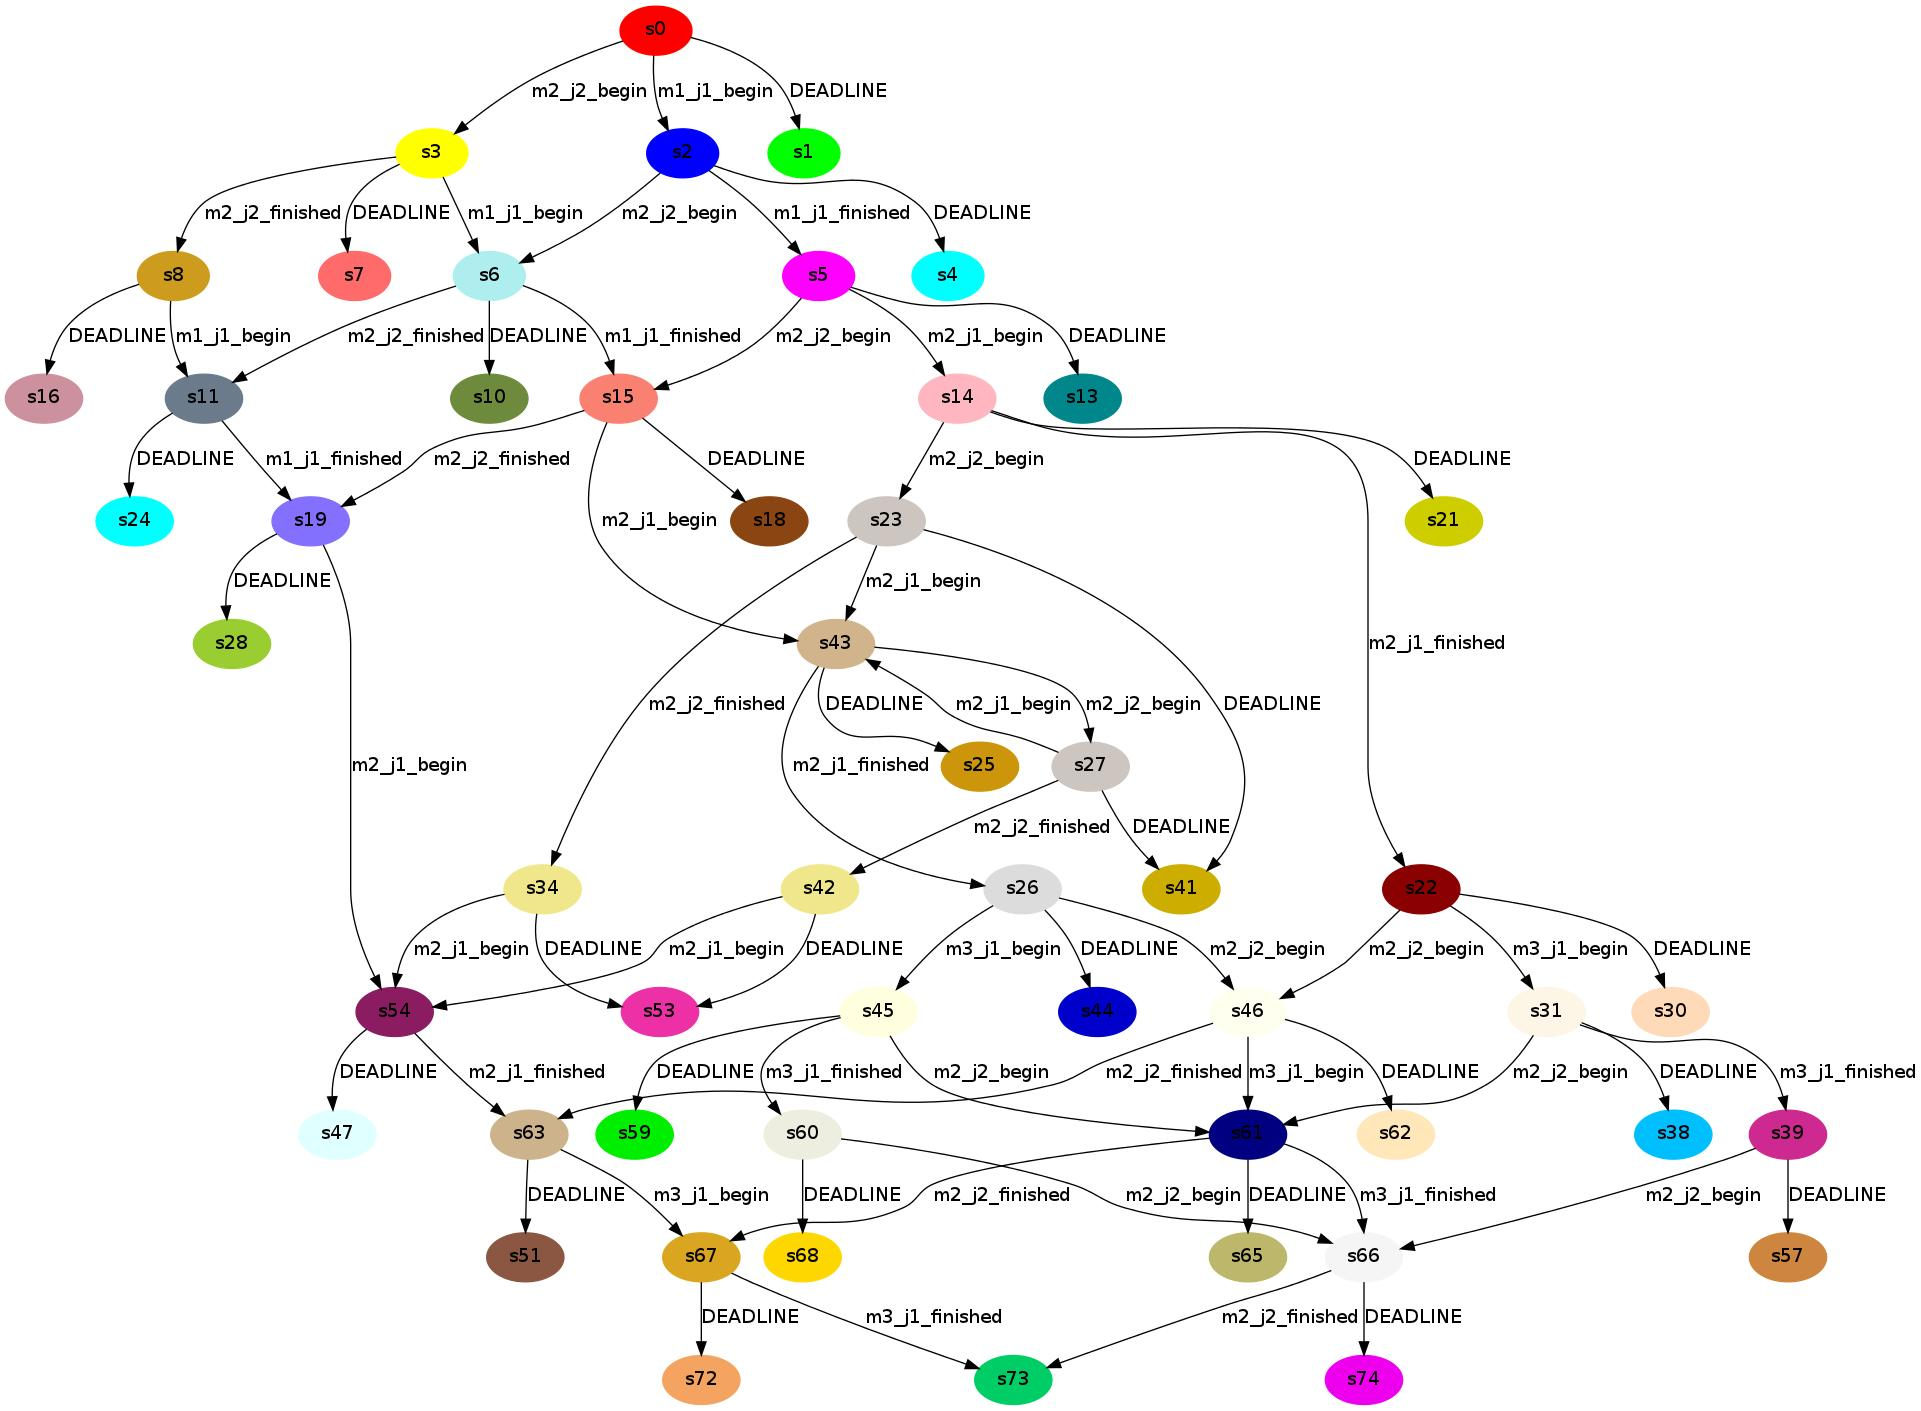
\includegraphics[scale = 0.12]{./figures/trace_set.jpg}
		\end{figure}
	\end{itemize}
\end{frame}
%%%%%%%%%%%%%%%%%%%%%%%%%%%%%%%%%%%%%%%%%%%%%%%%%%%%%%%%%%%%%%%%%%%%%%%%%%%%%%%%%



%%%%%%%%%%%%%%%%%%%%%%%%%%%%%%%%%%%%%%%%%%%%%%%%%%%%%%%%%%%%%%%%%%%%%%%%%%%%%%%%%
\begin{frame}
 \frametitle{What's Inside?}
\begin{itemize}
	\item \couleur{\imitator{}} 2.5 \refer{afks12}

	\begin{itemize}
		\item ``\couleur{I}nverse \couleur{M}ethod for \couleur{I}nferring \couleur{T}ime \couleur{A}bstrac\couleur{T} Behavi\couleur{OR}''
		\item 10\,000 lines of \couleur{\ocaml{}} code
		\item Makes use of the \couleur{PPL} library for handling polyhedra \refer{bhz08}
		\item Implements an efficient state \couleur{merging technique} \refer{AFS12}
		\item Numerous analysis \couleur{options}
	\end{itemize}

	\bigskip
% 
% 	\item Main contributors
% 
% 	\begin{itemize}
% 		\item \'Etienne Andr\'e
% 		\item Laurent Fribourg
% 		\item Ulrich K\"uhne
% 		\item Romain Soulat
% 	\end{itemize}

	\bigskip

	\item Available on the Web

	\begin{itemize}
		\item \couleur{\url{http://www.lsv.ens-cachan.fr/Software/imitator/}}
	\end{itemize}

% 	\pause
% 	
% 	\medskip
% 
% 	\item And now part of CosyVerif!


\end{itemize}

\end{frame}
%%%%%%%%%%%%%%%%%%%%%%%%%%%%%%%%%%%%%%%%%%%%%%%%%%%%%%%%%%%%%%%%%%%%%%%%%%%%%%%%%
%%%%%%%%%%%%%%%%%%%%%%%%%%%%%%%%%%%%%%%%%%%%%%%%%%%%%%%%%%%%%%%%%%%%%%%%%%%%%%%%%

\begin{frame}
\frametitle{Case Studies and Main Projects}

\begin{itemize}
	\item Applications

	\begin{itemize}
		\item Asynchronous circuits
		\begin{itemize}
			\item From the literature
			\item Model of an industrial circuit (ST-Microelectronics)
		\end{itemize}
		
		\smallskip
		
		\item Communication protocols

		\smallskip

		\item Scheduling problems \couleur{with preemption (feature of \imitator{} 2.5)}
		\begin{itemize}
			\item From the literature
			\item Model of the next generation of architecture for Arianne 6 (multi-processor, multi-partition, multi-tasks) with Astrium EADS
		\end{itemize}
	\end{itemize}
	
	\smallskip

	\item Set of case studies available on the Web page

% 	\bigskip
% 
% 	\item Industrial projects
% 
% 	\begin{itemize}
% 		\item ANR \couleur{Valmem} (with ST-Microelectronics) : 2007--2010 \refer{ACEF09}
% 		
% 		\medskip
% 		
% 		\item Farman \couleur{ROSCOV} (with EADS Astrium Space Transportation) : 2012--2013 \refer{FLMS12}
% 	\end{itemize}


\end{itemize}

\end{frame}



%%%%%%%%%%%%%%%%%%%%%%%%%%%%%%%%%%%%%%%%%%%%%%%%%%%%%%%%%%%%%%%%%%%%%%%%%%%%%%%%%
\section{Perspectives}
%%%%%%%%%%%%%%%%%%%%%%%%%%%%%%%%%%%%%%%%%%%%%%%%%%%%%%%%%%%%%%%%%%%%%%%%%%%%%%%%%
\begin{frame}
 \frametitle{Perspectives}
\begin{itemize}
%  \item Branch-and-bound strategy to cut branches that are to take longer than the deadline
% 	\item Integration in the CosyVerif platform

	\item Integration in the CosyVerif platform
	\begin{itemize}
		\item Graphical interface
		\item Eclipse plugin based on Web services
		\item \url{http://www.cosyverif.org/}
	\end{itemize}
\end{itemize}

\end{frame}
%%%%%%%%%%%%%%%%%%%%%%%%%%%%%%%%%%%%%%%%%%%%%%%%%%%%%%%%%%%%%%%%%%%%%%%%%%%%%%%%%







\backupbegin{}



\section*{\biblio{}}
%%%%%%%%%%%%%%%%%%%%%%%%%%%%%%%%%%%%%%%%%%%%%%%%%%%%%%%%%%%%%%%%%%%%%%%%%%%%%%%%%%
%%%%%%%%%%%%%%%%%%%%%%%%%%%%%%%%%%%%%%%%%%%%%%%%%%%%%%%%%%%%%%%%%%%%%%%%%%%%%%%%%%

%%%%%%%%%%%%%%%%%%%%%%%%%%%%%%%%%%%%%%%%%%%%%%%%%%%%%%%%%%%%%%%%%%%%%%%%%%%%%%%%%
%%%%%%%%%%%%%%%%%%%%%%%%%%%%%%%%%%%%%%%%%%%%%%%%%%%%%%%%%%%%%%%%%%%%%%%%%%%%%%%%%


%%%%%%%%%%%%%%%%%%%%%%%%%%%%%%%%%%%%%%%%%%%%%%%%%%%%%%%%%%%%%%%%%%%%%%%%%%%%%%%%%
\begin{frame}[allowframebreaks]
\frametitle{References}

% \nocite*{}

\scriptsize{
	\bibliographystyle{apalike} % alpha / apalike
	\bibliography{biblioIMI}
}

\end{frame}
%%%%%%%%%%%%%%%%%%%%%%%%%%%%%%%%%%%%%%%%%%%%%%%%%%%%%%%%%%%%%%%%%%%%%%%%%%%%%%%%%%
%%%%%%%%%%%%%%%%%%%%%%%%%%%%%%%%%%%%%%%%%%%%%%%%%%%%%%%%%%%%%%%%%%%%%%%%%%%%%%%%%%%%
%\section*{Experiments}
%\begin{frame}
%\frametitle{Experiments}
%\scalebox{0.7}{
%\begin{tabular}{|c|c|c|c|c|c|c|c|c|}
%\hline
% Case study             & $|\mathcal{A}|$& $|X|$ & $|P|$ & $|S|$        & $|T|$         & $n$   &
%$|K|$ & t               \\
%\hline
%jobshop $2\times 3$               & 4 & 6         & 8     & 676/3194      & 886/3931      & 15/15 & 15/10
%& 288.2/450.4   \\
%\hline
%jobshop $2\times 5$               & 4 & 6         & 8     & 676/3194      & 886/3931      & 15/15 & 15/10
%& 288.2/450.4   \\
%\hline
%jobshop $3\times 5$               & 4 & 6         & 8     & 676/3194      & 886/3931      & 15/15 & 15/10
%& 288.2/450.4   \\
%\hline
%cpr08 \cite{cpr08}               & 4 & 6         & 8     & 676/3194      & 886/3931      & 15/15 & 15/10
%& 288.2/450.4   \\
%\hline
%hppr10 \cite{LPPRC10}             & 3 & 4 &  9& 60/103    & 103/686               & 10/10 & 7/5 &
%2.10/11.7\\
%\hline
%Task chains \cite{SGL97} & 8 & 15 & 18 & 215/1364 & 264/1363 & 15/15 &
%17/17 & 85.3/270.6\\
%\hline
%%Astrium (RM) \cite{soulat12}       & 5 & 7         & 10    & 63/63         & 62/62         & 32/32 &
%%12/12 & 1.10/0.93       \\
%%\hline
%%RM 1            & 5 & 7         & 10    & 205/805       & 225/837       & 40/40 & 11/11 & 15.6/28.5  \\
%%\hline
%%RM 2            & 5 & 7         & 10    & 208/1174      & 228/1269      & 42/42 & 12/12 & 10.7/41.0  \\
%%\hline
%%RM 3            & 5 & 7         & 10    & 49/82         & 51/81         & 15/15 & 12/12 & 1.03/1.75  \\
%%\hline
%%Astrium (EDF)   & 5 & 10        & 13    & 63/63         & 62/62         & 32/32 & 13/13 &
%%2.42/2.30       \\
%%\hline
%EDF 1           & 5 & 10        & 13    & 76/415        & 91/454 & 31/31        & 20/20 & 66.1/288.2  \\
%\hline
%EDF 2           & 5 & 10        & 13    & 254/642       & 326/817       & 47/47 & 12/12 & 9.9/23.2  \\
%\hline
%EDF 3           & 5 & 10&  13   & 31/43         & 33/45         & 9/9   & 13/14 & 1.09/1.57  \\
%\hline
%\end{tabular}
%}
%
%
%\end{frame}
%%%%%%%%%%%%%%%%%%%%%%%%%%%%%%%%%%%%%%%%%%%%%%%%%%%%%%%%%%%%%%%%%%%%%%%%%%%%%%%%%%

\backupend{}



\end{document}
%%%%%%%%%%%%%%%%%%%%%%%%%%%%%%%%%%%%%%%%%%%%%%%%%%%%%%%%%%%%%%%%%%%%%%%%%%%%%%%%%
%%%%%%%%%%%%%%%%%%%%%%%%%%%%%%%%%%%%%%%%%%%%%%%%%%%%%%%%%%%%%%%%%%%%%%%%%%%%%%%%%
%%%%%%%%%%%%%%%%%%%%%%%%%%%%%%%%%%%%%%%%%%%%%%%%%%%%%%%%%%%%%%%%%%%%%%%%%%%%%%%%%










%%%%%%%%%%%%%%%%%%%%%%%%%%%%%%%%%%%%%%%%%%%%%%%%%%%%%%%%%%%%%%%%%%%%%%%%%%%%%%%%%%
%%%%%%%%%%%%%%%%%%%%%%%%%%%%%%%%%%%%%%%%%%%%%%%%%%%%%%%%%%%%%%%%%%%%%%%%%%%%%%%%%%
\section*{Introduction}
%%%%%%%%%%%%%%%%%%%%%%%%%%%%%%%%%%%%%%%%%%%%%%%%%%%%%%%%%%%%%%%%%%%%%%%%%%%%%%%%%%
%%%%%%%%%%%%%%%%%%%%%%%%%%%%%%%%%%%%%%%%%%%%%%%%%%%%%%%%%%%%%%%%%%%%%%%%%%%%%%%%%%
\begin{frame}
 \frametitle{An Example of a Jobshop Problem}
 \begin{figure}
  \centering
\begin{tikzpicture}[scale = 0.3,->,>=stealth',shorten >=1pt,auto,node distance=1.2cm,
                    semithick]
  \tikzstyle{every state}=[fill=red,draw=none,text=white]

    \node[initial,state] (A)                     {$J1_{start}$};
    \node[state]         (B)  [below of=A]    {On machine 1};
    \node[state]         (C) [below of=B]    {Machine 1 done};
    \node[state]         (D)  [below of=C]   {On machine 2};
    \node[state]         (E) [below of=D]    {Machine 2 done};
    \node[state]         (F)  [below of=E]   {On machine 3};
    \node[state]         (G) [below of=F]    {Machine 3 done};

 
 
   \path (A) edge node {$m_1 == 0$,$t1:=0$,$m_1 := 1$} (B)
 	(B) edge node {$t_1 == 3$,$m_1:= 0$} (C)
 	(C) edge node {$m_2 == 0$,$t1:=0$,$m_2 := 1$} (D)
 	(D) edge node {$t_1 == 2$,$m_2:= 0$} (E)
 	(E) edge node {$m_3 == 0$,$t1:=0$,$m_3 := 1$} (F)
 	(F) edge node {$t_1 == 4$,$m_1:= 0$} (G);

	
\end{tikzpicture}
\hspace{1cm}
\begin{tikzpicture}[->,>=stealth',shorten >=1pt,auto,node distance=1.2cm,
                    semithick]
  \tikzstyle{every state}=[fill=red,draw=none,text=white]

    \node[initial,state] (A) {$J2_{start}$};
    \node[state] 	 (B) [below of= A] {On machine 2};
    \node[state]	 (C) [below of= B] {Machine 2 done};	

  \path (A) edge node {$m_2 == 0$,$t2:=0$,$m_1 := 1$} (B)
 	(B) edge node {$t_2 == 5$,$m_2:= 0$} (C);
 
\end{tikzpicture}

 \end{figure}

\end{frame}

\begin{frame}

 \begin{figure}
  \centering
\begin{tikzpicture}[scale = 0.3,->,>=stealth',shorten >=1pt,auto,node distance=1.2cm,
                    semithick]
  \tikzstyle{every state}=[fill=red,draw=none,text=white]

    \node[initial,state] (A)                     {$J1_{start}$};
    \node[state]         (B)  [below of=A]    {On machine 1};
    \node[state]         (B') [left of=B]    {Preempted};
    \node[state]         (C) [below of=B]    {Machine 1 done};
    \node[state]         (D)  [below of=C]   {On machine 2};
    \node[state]         (D') [left of=D]    {Preempted};
    \node[state]         (E) [below of=D]    {Machine 2 done};
    \node[state]         (F)  [below of=E]   {On machine 3};
    \node[state]         (F') [left of=F]    {Preempted};
    \node[state]         (G) [below of=F]    {Machine 3 done};

 
 
   \path (A) edge node {$m_1 == 0$,$t1:=0$,$m_1 := 1$} (B)
 	(B) edge node {$t_1 == 3$,$m_1:= 0$} (C)
	    edge node {On hold} (B')
	(B') edge node {Released} (B)
 	(C) edge node {$m_2 == 0$,$t1:=0$,$m_2 := 1$} (D)
 	(D) edge node {$t_1 == 2$,$m_2:= 0$} (E)
	    edge node {On hold} (D')
	(D') edge node {Released} (D)
 	(E) edge node {$m_3 == 0$,$t1:=0$,$m_3 := 1$} (F)
 	(F) edge node {$t_1 == 4$,$m_1:= 0$} (G)
	    edge node {On hold} (F')
	(F') edge node {Released} (F);

	
\end{tikzpicture}
\hspace{1cm}
\begin{tikzpicture}[->,>=stealth',shorten >=1pt,auto,node distance=1.2cm,
                    semithick]
  \tikzstyle{every state}=[fill=red,draw=none,text=white]

    \node[initial,state] (A) {$J2_{start}$};
    \node[state] 	 (B) [below of= A] {On machine 2};
    \node[state]	 (C) [below of= B] {Machine 2 done};	

  \path (A) edge node {$m_2 == 0$,$t2:=0$,$m_1 := 1$} (B)
 	(B) edge node {$t_2 == 5$,$m_2:= 0$} (C);
 
\end{tikzpicture}

 \end{figure}
\end{frame}


%%%%%%%%%%%%%%%%%%%%%%%%%%%%%%%%%%%%%%%%%%%%%%%%%%%%%%%%%%%%%%%%%%%%%%%%%%%%%%%%%%
\begin{frame}
\frametitle{An Example of Flip-Flop Circuit}

\begin{itemize}
	\item An asynchronous circuit \refer{cc07}

	\begin{figure}
		\centering
% 		\includegraphics[width=0.4\textwidth]{flipflop.jpg}
	%-%-%-%-%-%-%-%-%-%-%-%-%-%-%-%-%-%-%-%-%-%-%-%-%-%-%-%-%-%-%
	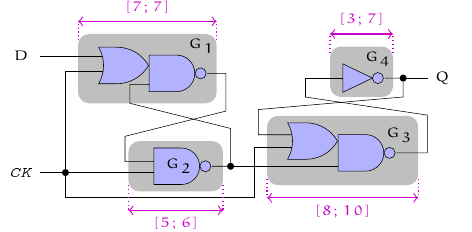
\begin{tikzpicture}[scale=.16,
		or/.style={or gate US, draw, very thin, fill=couleurfondclair, anchor=west},
		nand/.style={nand gate US, draw, very thin, fill=couleurfondclair, anchor=west},
		not/.style={not gate US, draw, very thin, fill=couleurfondclair, anchor=west},
		]
		\tiny
		% STYLES
		\tikzstyle{doublefleche} = [thin, <->, draw=violet]
		\tikzstyle{duree} = [below, pos=0.5, text=violet]
		\tikzstyle{fil} = [very thin, draw=black]
		\tikzstyle{point} = [scale=0.4, circle, fill=black]
		\tikzstyle{pointilles} = [thin, draw=violet, densely dotted]
		\tikzstyle{rectanglegris} = [rounded corners, fill=lightgray, draw=none]

		\path[use as bounding box] (-3, -8) rectangle (30, 6);

		% ELEMENT G1 : RECTANGLE
		\draw[rectanglegris] (1, 0) rectangle (12, 5.5);
		% ELEMENT G2 : RECTANGLE
		\draw[rectanglegris] (5, -7) rectangle (12.5, -3);
		% ELEMENT G3 : RECTANGLE
		\draw[rectanglegris] (16, -6.5) rectangle (28, -1);
		% ELEMENT G4 : RECTANGLE
		\draw[rectanglegris] (21, 0.5) rectangle (26, 4.5);

		% SIGNAL D
		\path [fil] (-2, 3.75) -- (3, 3.75);

		% ELEMENT G1 : PORTES
		\node[or] at (3, 3) [] (OR1) {};
		\node[nand, yshift=-0.1cm] at (OR1.east) (NAND1) {};
		\node[xshift=0.07cm] at (NAND1.east) (NAND1est) {};

		% FIL G1 - G2
		\path [fil] (NAND1est) --++ (2, 0) --++ (0, -3) --++ (-8, -2) --++ (0, -2) --++ (2.4, 0);

		% ELEMENT G2 : PORTES
		\node[nand] at (7, -5) (NAND2) {};
		\node[xshift=0.07cm] at (NAND2.east) (NAND2est) {};

		% FIL G2 - pointG2
	% 	\path [fil] (NAND2est) --++ (2, 0) --++ (0, +3) --++ (-8, +2) --++ (0, +1.5) --++ (1.60, 0);
		\path [fil] (NAND2est) --++ (2, 0) node [anchor=mid]  (pointG2) {};
		% FIL pointG2 - G1
		\path [fil] (pointG2.mid) --++ (0, +3) --++ (-8, +2) --++ (0, +1.5) --++ (1.60, 0);
		% POINT G2
		\node[point] at (pointG2.mid) {};

		% FIL pointG2 - G3
		\path [fil] (pointG2.mid) --++ (9, 0);

		% ELEMENT G4 : PORTE
		\node[not] at (22, 2) (NOT4) {};
		\node[xshift=0.07cm] at (NOT4.east) (NOT4est) {};

		% FIL G4 - pointG4
		\path [fil] (NOT4est) --++ (2, 0) node [anchor=mid]  (pointG4) {};
		% FIL G4 - inputG4
		\path [fil] (NOT4.west) --++ (-3, 0) --++ (0, -1.5) node [anchor=mid]  (inputG4) {};
		% FIL pointG2 - G1
	% 	\path [fil] (pointG2.mid) --++ (0, +3) --++ (-8, +2) --++ (0, +1.5) --++ (1.60, 0);
		% POINT G4
		\node[point] at (pointG4.mid) {};

		% FIL POINTG4 - G3
		\path [fil] (pointG4.mid) --++ (0, -1.5) --++ (-11.5, -1) --++ (0, -2) --++ (3, 0);

		% ELEMENT G3 : PORTES
		\node[or] at (18, -3) (OR3) {};
		\node[nand, yshift=-0.15cm] at (OR3.east) (NAND3) {};
		\node[xshift=0.07cm] at (NAND3.east) (NAND3est) {};

		% FIL G3 - input G4
		\path [fil] (NAND3est) --++ (3, 0) --++ (0, +3) -- (inputG4.mid);

		% SIGNAL Q
		\path [fil] (pointG4.mid) --++ (2, 0) node [anchor=mid] (nomQ) {};

		% SIGNAL CK
		\path [fil] (-2, -5.5) --++ (2, 0) node [anchor=mid]  (pointCK) {};
		% POINT CK
		\node[point] at (pointCK.mid) {};
		% FIL CK - G2
		\path [fil] (pointCK.mid) --++ (7, 0);
		% FIL CK - G1
		\path [fil] (pointCK.mid) --++ (0, 8) --++ (3, 0);
		% FIL CK - G3
		\path [fil] (pointCK.mid) --++ (0, -2) --++ (15, 0) --++ (0, 4) --++ (3, 0);

		% NOM DES SIGNAUX
		\node at (-3.5, 3.75) {$D$};
		\node at (-3.5, -5.5) {$\mathit{CK}$};
		\node[xshift=5] at (nomQ.mid) {$Q$};

		% NOM DES ELEMENTS
		\node at (10.8, 4.5) {$G_1$};
		\node at (9, -5) {$G_2$};
		\node at (26.5, -2.5) {$G_3$};
		\node at (24.8, 3.5) {$G_4$};
		
		% POINTILLES G1
		\path<2->[pointilles] (1, 5.0) --++ (0, 1.5) node (G1a) {};
		\path<2->[pointilles] (12, 5.0) --++ (0, 1.5) node (G1b) {};
		% POINTILLES G2
		\path<2->[pointilles] (5, -6.5) --++ (0, -2) node (G2a) {};
		\path<2->[pointilles] (12.5, -6.5) --++ (0, -2) node (G2b) {};
		% POINTILLES G3
		\path<2->[pointilles] (16, -6) --++ (0, -1.5) node (G3a) {};
		\path<2->[pointilles] (28, -6.0) --++ (0, -1.5) node (G3b) {};
		% POINTILLES G1
		\path<2->[pointilles] (21, 4) --++ (0, 1.5) node (G4a) {};
		\path<2->[pointilles] (26, 4) --++ (0, 1.5) node (G4b) {};
		
		% DUREES
		\path<2->[doublefleche] (G1a.base) -- (G1b.base) node[duree, above] {$[7; 7]$};
		\path<2->[doublefleche] (G2a.base) -- (G2b.base) node[duree, below] {$[5; 6]$};
		\path<2->[doublefleche] (G3a.base) -- (G3b.base) node[duree, below] {$[8; 10]$};
		\path<2->[doublefleche] (G4a.base) -- (G4b.base) node[duree, above] {$[3; 7]$};
		
	\end{tikzpicture}
	%-%-%-%-%-%-%-%-%-%-%-%-%-%-%-%-%-%-%-%-%-%-%-%-%-%-%-%-%-%-%
	\hspace{1.5cm}
	%-%-%-%-%-%-%-%-%-%-%-%-%-%-%-%-%-%-%-%-%-%-%-%-%-%-%-%-%-%-%
	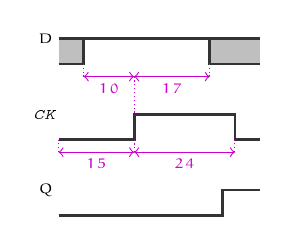
\begin{tikzpicture}[scale=.16]
		\tiny
		% STYLES
		\tikzstyle{signal} = [line width=1pt,draw=black!80]
		\tikzstyle{doublefleche} = [thin, <->, draw=violet]
		\tikzstyle{pointilles} = [thin, draw=violet, densely dotted]

		\tikzstyle{duree} = [below, pos=0.5, text=violet]

		\tikzstyle{fondgris} = [fill=lightgray, draw=none]

		% NOEUDS
		\node[] at (-1, 14) (D) {$D$};
		\node[] at (-1, 8) (CK) {$\mathit{CK}$};
		\node[] at (-1, 2) (Q) {$Q$};
		
		% D
		\draw[fondgris] (0, 12) rectangle (2, 14);
		\draw[fondgris] (12, 12) rectangle (16, 14);
		\path[signal]
			(0,14)
			-- ++ (16,0)
		;
		\path[signal]
			(0,12)
			-- ++ (2,0)
			-- ++ (0,2)
		;
		\path[signal]
			(12,14)
			-- ++ (0,-2)
			-- ++ (4,0)
		;

		\path<3->[doublefleche] (2, 11) -- ++(4, 0) node[duree] {$10$};
		\path<3->[doublefleche] (6, 11) -- ++(6, 0) node[duree] {$17$};
		\path<3->[pointilles] (2, 11) -- ++(0, 1);
		\path<3->[pointilles] (12, 11) -- ++(0, 1);

		% CK
		\path[signal]
			(0,6)
			-- ++ (6,0)
			-- ++ (0,2) 
			-- ++ (8,0)
			-- ++ (0,-2)
			-- ++ (2,0)
		;
		\path<3->[doublefleche] (0, 5) -- ++(6, 0) node[duree] {$15$};
		\path<3->[doublefleche] (6, 5) -- ++(8, 0) node[duree] {$24$};
		\path<3->[pointilles] (0, 5) -- ++(0, 1);
		\path<3->[pointilles] (14, 5) -- ++(0, 1);
		\path<3->[pointilles] (6, 11) -- ++(0, -3);
% 		\path[pointilles] (6, 6) -- ++(0, -3);
		\path<3->[pointilles] (6, 6) -- ++(0, -1);

		% Q
		\path[signal]
			(0,0)
			-- ++ (13,0)
			-- ++ (0,2) 
			-- ++ (3,0)
		;
	\end{tikzpicture}
	%-%-%-%-%-%-%-%-%-%-%-%-%-%-%-%-%-%-%-%-%-%-%-%-%-%-%-%-%-%-%
	\end{figure}




	\begin{itemize}
		\item Concurrent behavior
		\begin{itemize}
			\item 4 elements: $G_1$, $G_2$, $G_3$, $G_4$ % with internal signals $g_1$ to $g_4$
			\item 2 input signals ($D$ and $\mathit{CK}$), 1 output signal ($Q$)
		\end{itemize}

		\item<2-> \couleur{Timing delays}
		\begin{itemize}
			\item Traversal delays of the gates: one interval per gate
			\item<3-> Environment timing constants 
		\end{itemize}

	\end{itemize}

	\medskip

	\item<4-> \couleur{Question}
	\begin{itemize}
		\item For these timing delays, does the rise of $Q$ always occur before the fall of $\mathit{CK}$?
		\item<5-> Timed model checking gives the answer: \couleur{yes}
	\end{itemize}

\end{itemize}



\end{frame}
%%%%%%%%%%%%%%%%%%%%%%%%%%%%%%%%%%%%%%%%%%%%%%%%%%%%%%%%%%%%%%%%%%%%%%%%%%%%%%%%%%



%%%%%%%%%%%%%%%%%%%%%%%%%%%%%%%%%%%%%%%%%%%%%%%%%%%%%%%%%%%%%%%%%%%%%%%%%%%%%%%%%
\begin{frame}
\frametitle{Synthesis of Parameters}

\begin{itemize}
	\item More difficult problem: \couleur{find values of the timing delays} for which the system behaves well

	\bigskip

	\item Idea: reason with unknown constants or \couleur{parameters}
	
	\bigskip

	\item Interesting applications
	\begin{itemize}
		\item Ensure the \couleur{robustness} of the system
		\item Allow the designer to \couleur{optimize} timing delays
% 		\item Allow to \couleur{scale down} large timing constants
	\end{itemize}

	
	\bigskip


	\item Difficult problem
	\begin{itemize}
		\item Both concurrent behavior and timed behavior
		\item Undecidable in general
	\end{itemize}

\end{itemize}

\end{frame}
%%%%%%%%%%%%%%%%%%%%%%%%%%%%%%%%%%%%%%%%%%%%%%%%%%%%%%%%%%%%%%%%%%%%%%%%%%%%%%%%%%




%%%%%%%%%%%%%%%%%%%%%%%%%%%%%%%%%%%%%%%%%%%%%%%%%%%%%%%%%%%%%%%%%%%%%%%%%%%%%%%%%%
\begin{frame}
\frametitle{Flip-Flop Circuit: Timing Parameters }

\begin{itemize}
	\item An asynchronous circuit

	\begin{figure}
		\centering
% 		\includegraphics[width=0.4\textwidth]{flipflop.jpg}
	%-%-%-%-%-%-%-%-%-%-%-%-%-%-%-%-%-%-%-%-%-%-%-%-%-%-%-%-%-%-%
	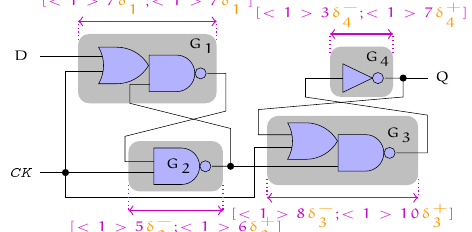
\begin{tikzpicture}[scale=.16,
		or/.style={or gate US, draw, very thin, fill=couleurfondclair, anchor=west},
		nand/.style={nand gate US, draw, very thin, fill=couleurfondclair, anchor=west},
		not/.style={not gate US, draw, very thin, fill=couleurfondclair, anchor=west},
		]
		\tiny
		% STYLES
		\tikzstyle{doublefleche} = [thin, <->, draw=violet]
		\tikzstyle{duree} = [below, pos=0.5, text=violet]
		\tikzstyle{fil} = [very thin, draw=black]
		\tikzstyle{point} = [scale=0.4, circle, fill=black]
		\tikzstyle{pointilles} = [thin, draw=violet, densely dotted]
		\tikzstyle{rectanglegris} = [rounded corners, fill=lightgray, draw=none]

		\path[use as bounding box] (-3, -8) rectangle (30, 6);

		% ELEMENT G1 : RECTANGLE
		\draw[rectanglegris] (1, 0) rectangle (12, 5.5);
		% ELEMENT G2 : RECTANGLE
		\draw[rectanglegris] (5, -7) rectangle (12.5, -3);
		% ELEMENT G3 : RECTANGLE
		\draw[rectanglegris] (16, -6.5) rectangle (28, -1);
		% ELEMENT G4 : RECTANGLE
		\draw[rectanglegris] (21, 0.5) rectangle (26, 4.5);

		% SIGNAL D
		\path [fil] (-2, 3.75) -- (3, 3.75);

		% ELEMENT G1 : PORTES
		\node[or] at (3, 3) [label=-20:G02] (OR1) {};
		\node[nand, yshift=-0.1cm] at (OR1.east) (NAND1) {};
		\node[xshift=0.07cm] at (NAND1.east) (NAND1est) {};

		% FIL G1 - G2
		\path [fil] (NAND1est) --++ (2, 0) --++ (0, -3) --++ (-8, -2) --++ (0, -2) --++ (2.4, 0);

		% ELEMENT G2 : PORTES
		\node[nand] at (7, -5) (NAND2) {};
		\node[xshift=0.07cm] at (NAND2.east) (NAND2est) {};

		% FIL G2 - pointG2
	% 	\path [fil] (NAND2est) --++ (2, 0) --++ (0, +3) --++ (-8, +2) --++ (0, +1.5) --++ (1.60, 0);
		\path [fil] (NAND2est) --++ (2, 0) node [anchor=mid]  (pointG2) {};
		% FIL pointG2 - G1
		\path [fil] (pointG2.mid) --++ (0, +3) --++ (-8, +2) --++ (0, +1.5) --++ (1.60, 0);
		% POINT G2
		\node[point] at (pointG2.mid) {};

		% FIL pointG2 - G3
		\path [fil] (pointG2.mid) --++ (9, 0);

		% ELEMENT G4 : PORTE
		\node[not] at (22, 2) (NOT4) {};
		\node[xshift=0.07cm] at (NOT4.east) (NOT4est) {};

		% FIL G4 - pointG4
		\path [fil] (NOT4est) --++ (2, 0) node [anchor=mid]  (pointG4) {};
		% FIL G4 - inputG4
		\path [fil] (NOT4.west) --++ (-3, 0) --++ (0, -1.5) node [anchor=mid]  (inputG4) {};
		% FIL pointG2 - G1
	% 	\path [fil] (pointG2.mid) --++ (0, +3) --++ (-8, +2) --++ (0, +1.5) --++ (1.60, 0);
		% POINT G4
		\node[point] at (pointG4.mid) {};

		% FIL POINTG4 - G3
		\path [fil] (pointG4.mid) --++ (0, -1.5) --++ (-11.5, -1) --++ (0, -2) --++ (3, 0);

		% ELEMENT G3 : PORTES
		\node[or] at (18, -3) (OR3) {};
		\node[nand, yshift=-0.15cm] at (OR3.east) (NAND3) {};
		\node[xshift=0.07cm] at (NAND3.east) (NAND3est) {};

		% FIL G3 - input G4
		\path [fil] (NAND3est) --++ (3, 0) --++ (0, +3) -- (inputG4.mid);

		% SIGNAL Q
		\path [fil] (pointG4.mid) --++ (2, 0) node [anchor=mid] (nomQ) {};

		% SIGNAL CK
		\path [fil] (-2, -5.5) --++ (2, 0) node [anchor=mid]  (pointCK) {};
		% POINT CK
		\node[point] at (pointCK.mid) {};
		% FIL CK - G2
		\path [fil] (pointCK.mid) --++ (7, 0);
		% FIL CK - G1
		\path [fil] (pointCK.mid) --++ (0, 8) --++ (3, 0);
		% FIL CK - G3
		\path [fil] (pointCK.mid) --++ (0, -2) --++ (15, 0) --++ (0, 4) --++ (3, 0);

		% NOM DES SIGNAUX
		\node at (-3.5, 3.75) {$D$};
		\node at (-3.5, -5.5) {$\mathit{CK}$};
		\node[xshift=5] at (nomQ.mid) {$Q$};

		% NOM DES ELEMENTS
		\node at (10.8, 4.5) {$G_1$};
		\node at (9, -5) {$G_2$};
		\node at (26.5, -2.5) {$G_3$};
		\node at (24.8, 3.5) {$G_4$};
		
		% POINTILLES G1
		\path[pointilles] (1, 5.0) --++ (0, 1.5) node (G1a) {};
		\path[pointilles] (12, 5.0) --++ (0, 1.5) node (G1b) {};
		% POINTILLES G2
		\path[pointilles] (5, -6.5) --++ (0, -2) node (G2a) {};
		\path[pointilles] (12.5, -6.5) --++ (0, -2) node (G2b) {};
		% POINTILLES G3
		\path[pointilles] (16, -6) --++ (0, -1.5) node (G3a) {};
		\path[pointilles] (28, -6.0) --++ (0, -1.5) node (G3b) {};
		% POINTILLES G1
		\path[pointilles] (21, 4) --++ (0, 1.5) node (G4a) {};
		\path[pointilles] (26, 4) --++ (0, 1.5) node (G4b) {};
		
		% DUREES
% 		\path[doublefleche] (G1a.base) -- (G1b.base) node[duree, above] {$[\alt<1>{7}{\coulparam{\delta_1^-}}; \alt<1>{7}{\coulparam{\delta_1^+}}]$};
% 		\path[doublefleche] (G2a.base) -- (G2b.base) node[duree, below] {$[\alt<1>{5}{\coulparam{\delta_2^-}}; \alt<1>{6}{\coulparam{\delta_2^+}}]$};
% 		\path[doublefleche] (G3a.base) -- (G3b.base) node[duree, below] {$[\alt<1>{8}{\coulparam{\delta_3^-}}; \alt<1>{10}{\coulparam{\delta_3^+}}]$};
% 		\path[doublefleche] (G4a.base) -- (G4b.base) node[duree, above] {$[\alt<1>{3}{\coulparam{\delta_4^-}}; \alt<1>{7}{\coulparam{\delta_4^+}}]$};
		\path[doublefleche] (G1a.base) -- (G1b.base) node[duree, above] {
			\begin{tabular}{@{} c @{} c @{} c @{} c @{} c @{}}
				& \ \ \ \ \ \ \ \ & & \ \ \ \ \ \ \ \ & \\
				$[$ & $\alt<1>{7}{\coulparam{\delta_1^-}}$ & $;$ & $\alt<1>{7}{\coulparam{\delta_1^+}}$ & $]$ \\
			\end{tabular}};
		\path[doublefleche] (G2a.base) -- (G2b.base) node[duree, below] {
			\begin{tabular}{@{} c @{} c @{} c @{} c @{} c @{}}
				$[$ & $\alt<1>{5}{\coulparam{\delta_2^-}}$ & $;$ & $\alt<1>{6}{\coulparam{\delta_2^+}}$ & $]$ \\
				& \ \ \ \ \ \ \ \ & & \ \ \ \ \ \ \ \ & 
			\end{tabular}};
		\path[doublefleche] (G3a.base) -- (G3b.base) node[duree, below] {
			\begin{tabular}{@{} c @{} c @{} c @{} c @{} c @{}}
				$[$ & $\alt<1>{8}{\coulparam{\delta_3^-}}$ & $;$ & $\alt<1>{10}{\coulparam{\delta_3^+}}$ & $]$ \\
				& \ \ \ \ \ \ \ \ & & \ \ \ \ \ \ \ \ & 
			\end{tabular}};
		\path[doublefleche] (G4a.base) -- (G4b.base) node[duree, above] {
			\begin{tabular}{@{} c @{} c @{} c @{} c @{} c @{}}
				& \ \ \ \ \ \ \ \ & & \ \ \ \ \ \ \ \ & \\
				$[$ & $\alt<1>{3}{\coulparam{\delta_4^-}}$ & $;$ & $\alt<1>{7}{\coulparam{\delta_4^+}}$ & $]$ \\
			\end{tabular}};
		
	\end{tikzpicture}
	%-%-%-%-%-%-%-%-%-%-%-%-%-%-%-%-%-%-%-%-%-%-%-%-%-%-%-%-%-%-%
	\hspace{1.5cm}
	%-%-%-%-%-%-%-%-%-%-%-%-%-%-%-%-%-%-%-%-%-%-%-%-%-%-%-%-%-%-%
	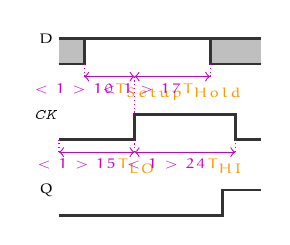
\begin{tikzpicture}[scale=.16]
		\tiny
		% STYLES
		\tikzstyle{signal} = [line width=1pt,draw=black!80]
		\tikzstyle{doublefleche} = [thin, <->, draw=violet]
		\tikzstyle{pointilles} = [thin, draw=violet, densely dotted]

		\tikzstyle{duree} = [below, pos=0.5, text=violet]

		\tikzstyle{fondgris} = [fill=lightgray, draw=none]

		% NOEUDS
		\node[] at (-1, 14) (D) {$D$};
		\node[] at (-1, 8) (CK) {$\mathit{CK}$};
		\node[] at (-1, 2) (Q) {$Q$};
		
		% D
		\draw[fondgris] (0, 12) rectangle (2, 14);
		\draw[fondgris] (12, 12) rectangle (16, 14);
		\path[signal]
			(0,14)
			-- ++ (16,0)
		;
		\path[signal]
			(0,12)
			-- ++ (2,0)
			-- ++ (0,2)
		;
		\path[signal]
			(12,14)
			-- ++ (0,-2)
			-- ++ (4,0)
		;

		\path[doublefleche] (2, 11) -- ++(4, 0) node[duree] {$\alt<1>{10}{\coulparam{\TSetup}}$};
		\path[doublefleche] (6, 11) -- ++(6, 0) node[duree] {$\alt<1>{17}{\coulparam{\THold}}$};
		\path[pointilles] (2, 11) -- ++(0, 1);
		\path[pointilles] (12, 11) -- ++(0, 1);

		% CK
		\path[signal]
			(0,6)
			-- ++ (6,0)
			-- ++ (0,2) 
			-- ++ (8,0)
			-- ++ (0,-2)
			-- ++ (2,0)
		;
		\path[doublefleche] (0, 5) -- ++(6, 0) node[duree] {$\alt<1>{15}{\coulparam{\TLO}}$};
		\path[doublefleche] (6, 5) -- ++(8, 0) node[duree] {$\alt<1>{24}{\coulparam{\THI}}$};
		\path[pointilles] (0, 5) -- ++(0, 1);
		\path[pointilles] (14, 5) -- ++(0, 1);
		\path[pointilles] (6, 11) -- ++(0, -3);
% 		\path[pointilles] (6, 6) -- ++(0, -3);
		\path[pointilles] (6, 6) -- ++(0, -1);

		% Q
		\path[signal]
			(0,0)
			-- ++ (13,0)
			-- ++ (0,2) 
			-- ++ (3,0)
		;
	\end{tikzpicture}
	%-%-%-%-%-%-%-%-%-%-%-%-%-%-%-%-%-%-%-%-%-%-%-%-%-%-%-%-%-%-%
	\end{figure}

	\medskip


% 	\begin{itemize}
% 		\item 4 elements: $G_1$, $G_2$, $G_3$, $G_4$ % with internal signals $g_1$ to $g_4$
% 		
% 		\smallskip
% 
% 		\item 2 input signals ($D$ and $\mathit{CK}$), 1 output signal ($Q$)
% 	\end{itemize}
% 
% 	\medskip

	\item<2-> \coulparam{Timing parameters}
	\begin{itemize}
		\item Traversal delays of the gates: one interval per gate % by the electric current
% 		\begin{itemize}
% 			\item Example for $G_1$: $[\coulparam{\delta_1^-}, \coulparam{\delta_1^+}]$
% 		\end{itemize}
		
		\smallskip
		
		\item 4 environment parameters: $\coulparam{\TLO}$, $\coulparam{\THI}$, $\coulparam{\TSetup}$ and $\coulparam{\THold}$
% 		Durations of low (\coulparam{$\TLO$}) and high (\coulparam{$\THI$}) levels of $\mathit{CK}$
% 
% 		\smallskip
% 		
% 		\item Stabilization time of $D$: \coulparam{$\TSetup$}, \coulparam{$\THold$}
	\end{itemize}
	
	\bigskip

	\item<3-> \couleur{Question}: for which values of the parameters does the rise of $Q$ always occur before the fall of $\mathit{CK}$?


\end{itemize}



\end{frame}
%%%%%%%%%%%%%%%%%%%%%%%%%%%%%%%%%%%%%%%%%%%%%%%%%%%%%%%%%%%%%%%%%%%%%%%%%%%%%%%%%%






%%%%%%%%%%%%%%%%%%%%%%%%%%%%%%%%%%%%%%%%%%%%%%%%%%%%%%%%%%%%%%%%%%%%%%%%%%%%%%%%%
\begin{frame}
\frametitle{Problems}

% We consider a system modeled by a parametric timed automaton. %~$\A$.

\begin{itemize}
	\item \couleur{The good parameters problem}
	
	\begin{itemize}
		\item ``Given a \couleur{bounded parameter domain} $\Vo$, find a set of parameter valuations of \couleur{good} behavior in~$\Vo$'' % (ideally the largest one)
	\end{itemize}
	

	% %-%-%-%-%-%-%-%-%-%-%-%-%-%-%-%-%-%-%-%-%-%-%-%-%-%-%-%-%-%-%
	\begin{figure}
	{

	\centering
	\footnotesize

	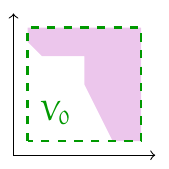
\begin{tikzpicture}[scale=0.18]

% 		\path[use as bounding box] (-1,-1) rectangle (1,1);
		\path[use as bounding box] (-4, -4) rectangle (4, 4);
		\draw<2->[fill=outputcolor!25, draw=none]
			(2, -4) -- (0, 0) -- (0, 2) -- (-3, 2) -- (-4, 3) -- (-4, 4) -- (4, 4) -- (4, -4) -- cycle;

% 		\node<2-> (k) at (2, 2) [text=outputcolor] {\large{$\Ko$}};

		% VO
		\tikzstyle{v0} = [line width=1pt, draw=inputcolor, dashed]
		\path[v0] (-4, -4) -- (-4, 4) -- (4, 4) -- (4, -4) -- cycle;
		\node (v0) at (-2, -2) [text=inputcolor] {$\Vo$};

		\draw[->] (-5, -5) -- (-5, 5);
		\draw[->] (-5, -5) -- (5, -5);
		

	\end{tikzpicture}

	}
	\end{figure}
	% %-%-%-%-%-%-%-%-%-%-%-%-%-%-%-%-%-%-%-%-%-%-%-%-%-%-%-%-%-%-%
	
% 	\bigskip

	\item<3-> The \couleur{inverse problem}: A simpler problem
	\begin{itemize}
		\item ``Given a \couleur{reference parameter valuation} $\pio$, find other valuations around $\pio$ of \couleur{same} behavior''
	\end{itemize}
	
	% %-%-%-%-%-%-%-%-%-%-%-%-%-%-%-%-%-%-%-%-%-%-%-%-%-%-%-%-%-%-%
	\begin{figure}
	{

	\centering
	\footnotesize

	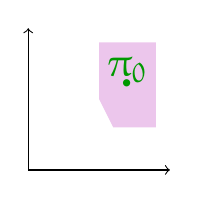
\begin{tikzpicture}[scale=0.18]

		\draw[->] (-5, -5) -- (-5, 5);
		\draw[->] (-5, -5) -- (5, -5);
		
		\path[use as bounding box] (-1,-1) rectangle (1,1);
% 		\draw<4->[fill=outputcolor!25, draw=none]
% 			(-3, -3) -- (-4, 3) -- (-2, 4) -- (3, 3) -- (5, 0) -- (3, -4) -- cycle;
		\draw<4->[fill=outputcolor!25, draw=none]
			(1, -2) -- (0, 0) -- (0, 4) -- (4, 4) -- (4, -2) -- cycle;

% 		\node<4-> (k) at (-1,-2) {\large{$\Ko$}};
		\node (point) at (2, 1) {\Huge{$\coulinput{\cdot}$}};
		\node (pi) at (2, 2) {\Large{$\pio$}};

	\end{tikzpicture}

	}
	\end{figure}
	% %-%-%-%-%-%-%-%-%-%-%-%-%-%-%-%-%-%-%-%-%-%-%-%-%-%-%-%-%-%-%

\end{itemize}

\end{frame}
%%%%%%%%%%%%%%%%%%%%%%%%%%%%%%%%%%%%%%%%%%%%%%%%%%%%%%%%%%%%%%%%%%%%%%%%%%%%%%%%%%





%%%%%%%%%%%%%%%%%%%%%%%%%%%%%%%%%%%%%%%%%%%%%%%%%%%%%%%%%%%%%%%%%%%%%%%%%%%%%%%%%%%
% Plan
\begin{frame}
	\frametitle{\plan{}}
	\tableofcontents[hideallsubsections]
\end{frame}
%%%%%%%%%%%%%%%%%%%%%%%%%%%%%%%%%%%%%%%%%%%%%%%%%%%%%%%%%%%%%%%%%%%%%%%%%%%%%%%%%%


%%%%%%%%%%%%%%%%%%%%%%%%%%%%%%%%%%%%%%%%%%%%%%%%%%%%%%%%%%%%%%%%%%%%%%%%%%%%%%%%%%
%%%%%%%%%%%%%%%%%%%%%%%%%%%%%%%%%%%%%%%%%%%%%%%%%%%%%%%%%%%%%%%%%%%%%%%%%%%%%%%%%%
\section{The Inverse Method}
%%%%%%%%%%%%%%%%%%%%%%%%%%%%%%%%%%%%%%%%%%%%%%%%%%%%%%%%%%%%%%%%%%%%%%%%%%%%%%%%%%
%%%%%%%%%%%%%%%%%%%%%%%%%%%%%%%%%%%%%%%%%%%%%%%%%%%%%%%%%%%%%%%%%%%%%%%%%%%%%%%%%%


%%%%%%%%%%%%%%%%%%%%%%%%%%%%%%%%%%%%%%%%%%%%%%%%%%%%%%%%%%%%%%%%%%%%%%%%%%%%%%%%%%%
% Plan
\begin{frame}
	\frametitle{\plan{}}
	\tableofcontents[currentsection, hideallsubsections]
\end{frame}
%%%%%%%%%%%%%%%%%%%%%%%%%%%%%%%%%%%%%%%%%%%%%%%%%%%%%%%%%%%%%%%%%%%%%%%%%%%%%%%%%%


%%%%%%%%%%%%%%%%%%%%%%%%%%%%%%%%%%%%%%%%%%%%%%%%%%%%%%%%%%%%%%%%%%%%%%%%%%%%%%%%%%
\begin{frame}
\frametitle{Functional view of \imitator{}}


%-%-%-%-%-%-%-%-%-%-%-%-%-%-%-%-%-%-%-%-%-%-%-%-%-%-%-%-%-%-%
	% STYLES
	\tikzstyle{etiquette} = [draw=none, color=black]
	
	\tikzstyle{boite}=[rectangle, draw=black, rounded corners, thick, draw=blue!40!black, top color=blue!5!white, bottom color=blue!20]
	\tikzstyle{fleche} = [->, draw=black, semithick]
{

\centering

\begin{tikzpicture}[scale=0.6,  =>stealth']

	\small

	% Boites
	\draw[boite] (-6, 5.5) rectangle (-2, 6.5);
	\node [etiquette] at (-4, 6) {PTA~$\A$};
	
	\draw[boite] (-6, 3.5) rectangle (-2, 5);
	\node [etiquette] at (-4, 4.25) {\begin{tabular}{c}Reference\\valuation $\pio$\end{tabular}};
	
	\draw[boite] (0, 4) rectangle (6, 6.5);
	\node [etiquette] at (3, 5.25) {\large \imitator{}};
	
% 	\draw[boite] (1, 4) rectangle (5, 5);
% 	\node [etiquette] at (3, 4.5) {PPL};
	
	\draw[boite] (8, 4.5) rectangle (12, 6);
	\node [etiquette] at (10, 5.25) {Constraint $\Ko$};
	
% 	\draw[boite] (8, 4) rectangle (12, 5);
% 	\node [etiquette] at (10, 4.5) {Trace set};

	% Fleches
	\path[fleche] (-2, 6) --++ (2, 0);
	\path[fleche] (-2, 4.4) --++ (2, 0);
% 	\path[fleche] (3.5, 4) --++ (0, -.5);
% 	\path[fleche] (2.5, 3.5) --++ (0, .5);
	\path[fleche] (6, 5.25) --++ (2, 0);
% 	\path[fleche] (6, 4.5) --++ (2, 0);

\end{tikzpicture}

}
%-%-%-%-%-%-%-%-%-%-%-%-%-%-%-%-%-%-%-%-%-%-%-%-%-%-%-%-%-%-%


\end{frame}
%%%%%%%%%%%%%%%%%%%%%%%%%%%%%%%%%%%%%%%%%%%%%%%%%%%%%%%%%%%%%%%%%%%%%%%%%%%%%%%%%%





%%%%%%%%%%%%%%%%%%%%%%%%%%%%%%%%%%%%%%%%%%%%%%%%%%%%%%%%%%%%%%%%%%%%%%%%%%%%%%%%%%
\begin{frame}
\frametitle{Trace Set}

\begin{itemize}
	\item \couleur{Trace set}: set of all traces of a PTA

	\bigskip

	\item Graphical representation under the form of a \couleur{tree}
	
	\begin{itemize}
		\item Does not give any information on the \couleur{branching behavior} though

		\medskip

		\item Example of trace set for the flip-flop example
	\end{itemize}

%-%-%-%-%-%-%-%-%-%-%-%-%-%-%-%-%-%-%-%-%-%-%-%-%-%-%-%-%-%-%
{
\centering
\footnotesize

\begin{tikzpicture}[scale=0.45, ->, >=stealth', shorten >=1pt, auto, thin]
\tikzstyle{state}=[circle, minimum size=12pt, draw=none, text=black, shade=ball, inner sep=1.5pt]

	\node[state, ball color=cv1] (Q0) at (0,4) {};
	\node[state, ball color=cv2]         (Q1) at (3,4) {};
	\node[state, ball color=cv3]         (Q2) at (6,4) {};
	\node[state, ball color=cv4]         (Q3) at (9,4) {};
% 	\node[state, fill=cpale5]         (Q4) at (12,4) {$q_4$};
	\node[state, ball color=cv5]         (Q5) at (12,4) {};
% 	\node[state, fill=cpale7]         (Q6) at (15,4) {$q_6$};
% 	\node[state, fill=cpale8]         (Q7) at (15,2) {$q_7$};
	\node[state, ball color=cv7]         (Q8) at (15,4) {};
	\node[state, ball color=cv6]         (Q9) at (15,6) {};
% 	\node[state, fill=cpale10]        (Q10) at (18,0) {$q_{10}$};
% 	\node[state, fill=cpale11]        (Q11) at (18,2) {$q_{11}$};
% 	\node[state, fill=cpale10]        (Q12) at (18,4) {$q_{12}$};
	\node[state, ball color=cv8]        (Q13) at (18,4) {};
	\node[state, ball color=cv8]        (Q14) at (18,6) {};
	\node[state, ball color=cv9]        (Q15) at (21,4) {};
% 	\node[state, fill=cpale12]        (Q16) at (21,4) {$q_{16}$};
% 	\node[state, fill=cpale12]        (Q17) at (21,2) {$q_{17}$};
% 	\node[state, fill=cpale12]        (Q18) at (21,0) {$q_{18}$};
	\node[state, ball color=cv9]        (Q19) at (21,6) {};

	\path
		(Q0) edge [double] node {$\coulact{D^\uparrow}$} (Q1)
		(Q1) edge [double] node {$\coulact{G_1^\downarrow}$} (Q2)
		(Q2) edge [double] node {$\coulact{\mathit{CK}^\uparrow}$} (Q3)
% 		(Q3) edge [double, below] node {$D^\downarrow$} (Q4)
		(Q3) edge [double] node {$\coulact{G_3^\downarrow}$} (Q5)
% 		(Q4) edge [double, below] node {$G_3^\downarrow$} (Q7)
% 		(Q4) edge [double] node {$\mathit{CK}^\downarrow$} (Q6)
		(Q5) edge [double] node {$\coulact{D^\downarrow}$} (Q8)
		(Q5) edge [double] node {$\coulact{Q^\uparrow}$} (Q9)
% 		(Q7) edge [double, below left] node {$\mathit{CK}^\downarrow$} (Q10)
% 		(Q7) edge [double] node {$Q^\uparrow$} (Q11)
% 		(Q8) edge [double, below] node {$\mathit{CK}^\downarrow$} (Q12)
		(Q8) edge [double] node {$\coulact{Q^\uparrow}$} (Q13)
		(Q9) edge [double] node {$\coulact{D^\downarrow}$} (Q14)
% 		(Q10) edge [double] node {$Q^\uparrow$} (Q18)
% 		(Q11) edge [double] node {$\mathit{CK}^\downarrow$} (Q17)
% 		(Q12) edge [double] node {$Q^\uparrow$} (Q16)
		(Q13) edge [double] node {$\coulact{\mathit{CK}^\downarrow}$} (Q15)
		(Q14) edge [double] node {$\coulact{\mathit{CK}^\downarrow}$} (Q19)
		;

\end{tikzpicture}

}
%-%-%-%-%-%-%-%-%-%-%-%-%-%-%-%-%-%-%-%-%-%-%-%-%-%-%-%-%-%-%



\end{itemize}

\end{frame}
%%%%%%%%%%%%%%%%%%%%%%%%%%%%%%%%%%%%%%%%%%%%%%%%%%%%%%%%%%%%%%%%%%%%%%%%%%%%%%%%%%




%%%%%%%%%%%%%%%%%%%%%%%%%%%%%%%%%%%%%%%%%%%%%%%%%%%%%%%%%%%%%%%%%%%%%%%%%%%%%%%%%%
\begin{frame}
\frametitle{The Inverse Method}

\begin{itemize}

	\item \coulinput{Input}
	\begin{itemize}
		\item A PTA $\A$ % with initial state \symb{$s_{\mathit{init}}$}
		\item A \couleur{reference valuation} $\pio$ of all the parameters of $\A$
% 		\begin{itemize}
%  			\item Exemplifying a good behavior\\
% 			(all traces of \symb{$\A[\pio]$} correspond to good behaviors)
% 		\end{itemize}
	\end{itemize}

	\bigskip

	\item<2-> \couloutput{Output: tile $\Ko$}
	\begin{itemize}
		\item Convex \couleur{constraint} on the parameters such that
		\begin{itemize}
			\item $\pio \models \Ko$
			\item For all points $\pi \models \Ko$, $\A[\pi]$ and $\A[\pio]$ have the \couleur{same trace sets}
		\end{itemize}
	\end{itemize}
\end{itemize}

\bigskip

% %-%-%-%-%-%-%-%-%-%-%-%-%-%-%-%-%-%-%-%-%-%-%-%-%-%-%-%-%-%-%
\begin{figure}
{

\centering
\footnotesize

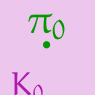
\begin{tikzpicture}[scale=0.25]

	\path[use as bounding box] (-1,-1) rectangle (1,1);
%     \node<2-> (patate) at (0,0) [regular polygon, regular polygon sides=5, minimum height=6em, fill=outputcolor!25] {};
%     \node (patate) at (0,0) [regular polygon, regular polygon sides=5, minimum height=6em, ] {};
	\draw<2->[fill=outputcolor!25, draw=none]
		(-3, -3) -- (-4, 3) -- (-2, 4) -- (3, 3) -- (5, 0) -- (3, -4) -- cycle;

	\node<2-> (k) at (-1,-2) {\large{$\Ko$}};
	\node (point) at (0,0) {\Huge{$\coulinput{\cdot}$}};
	\node (pi) at (0,1) {\Large{$\pio$}};

\end{tikzpicture}

}
\end{figure}
% %-%-%-%-%-%-%-%-%-%-%-%-%-%-%-%-%-%-%-%-%-%-%-%-%-%-%-%-%-%-%

\end{frame}
%%%%%%%%%%%%%%%%%%%%%%%%%%%%%%%%%%%%%%%%%%%%%%%%%%%%%%%%%%%%%%%%%%%%%%%%%%%%%%%%%%





%%%%%%%%%%%%%%%%%%%%%%%%%%%%%%%%%%%%%%%%%%%%%%%%%%%%%%%%%%%%%%%%%%%%%%%%%%%%%%%%%%
\begin{frame}
\frametitle{The Inverse Method: General Idea}

\begin{itemize}
	\item The idea \refer{ACEF09}
	\begin{itemize}
		\item Instead of negating bad states (as in ``CEGAR'' approaches), we remove \couleur{$\pio$-incompatible} states
	\end{itemize}
\end{itemize}


%-%-%-%-%-%-%-%-%-%-%-%-%-%-%-%-%-%-%-%-%-%-%-%-%-%-%-%-%-%-%
{
\centering
\footnotesize

\begin{tikzpicture}[>=stealth', node distance=3cm, semithick]
	\tikzstyle{state} = [circle, minimum size=12pt, draw=none, shade=ball, inner sep=1.5pt]
	\tikzstyle{contrainte}=[rectangle, draw=couleurgood, inner sep=1pt, text width=2cm, font=\scriptsize]
	\tikzstyle{transition} = [->, double]
	\tikzstyle{liaison} = [-, dashed]
	\tikzstyle{croix} = [thick, draw=couleurbad]

	\path[use as bounding box] (-1, -0.5) rectangle (7, 3);

	% ETATS
	\node[state, ball color=cv1] at (0, 0) (Q0) {};
	\node[state, ball color=cv2] at (2.5, 0) (Q1) {};
	\node[state, ball color=cv3] at (5, 0) (Q2) {};
	\node[state, ball color=cv4] at (5, 1) (Q3) {};

	% CONTRAINTES
	\node[contrainte, fill=cv1!30] at (0, -1) (C0) {\centering \begin{tabular}{r @{\,} c @{\,} l }
		$\coulparam{d_1}$ & $\leq$ & $\coulparam{d_2}$ \\
		& & \\
	\end{tabular}
	
	};

	\node[contrainte, fill=cv2!30] at (2.5, -1) (C1) {\centering \begin{tabular}{r @{\,} c @{\,} l }
		$\coulparam{d_1}$ & $\leq$ & $\coulparam{d_2}$ \\
		$\coulparam{d_1}$ & $\leq$ & $\coulparam{d_3} + \coulparam{d_4}$ \\
	\end{tabular}
	};

	\node[contrainte, fill=cv3!30] at (5, -1) (C2) {\centering \begin{tabular}{r @{\,} c @{\,} l }
		$\coulparam{d_1}$ & $\leq$ & $\coulparam{d_2}$ \\
		$\coulparam{d_1}$ & $\leq$ & $\coulparam{d_3} + \coulparam{d_4}$ \\
		$\coulparam{d_3}$ & $\geq$ & $\coulparam{d_4}$ \\
	\end{tabular}	
	};

	\node[contrainte, fill=cv4!30, draw=couleurbad] at (5, 2) (C3) {\centering \begin{tabular}{r @{\,} c @{\,} l }
		$\coulparam{d_1}$ & $\leq$ & $\coulparam{d_2}$ \\
		$\coulparam{d_1}$ & $\leq$ & $\coulparam{d_3} + \coulparam{d_4}$ \\
		$\textcolor{red}{d_3}$ & $\textcolor{red}{<}$ & $\textcolor{red}{d_4}$ \\
	\end{tabular}	
	};


	% TRANSITIONS
	\path (Q0) edge [transition, above] node {$\coulact{a}$} (Q1);
	\path (Q1) edge [transition, above] node {$\coulact{b}$} (Q2);
	\path (Q1) edge [transition, above] node {$\coulact{c}$} (Q3);

	% LIAISONS
	\path (Q0) edge [liaison] (C0);
	\path (Q1) edge [liaison] (C1);
	\path (Q2) edge [liaison] (C2);
	\path (Q3) edge [liaison] (C3);
	
	% CROIX
% 	\path (4, 3) edge [croix] (6, 1);
% 	\path (4, 1) edge [croix] (6, 3);
	\path<2-> (3.5, 3) edge [croix] (6.5, 0.5);
	\path<2-> (3.5, 0.5) edge [croix] (6.5, 3);


\end{tikzpicture}

}
%-%-%-%-%-%-%-%-%-%-%-%-%-%-%-%-%-%-%-%-%-%-%-%-%-%-%-%-%-%-%



\end{frame}
%%%%%%%%%%%%%%%%%%%%%%%%%%%%%%%%%%%%%%%%%%%%%%%%%%%%%%%%%%%%%%%%%%%%%%%%%%%%%%%%%%




%%%%%%%%%%%%%%%%%%%%%%%%%%%%%%%%%%%%%%%%%%%%%%%%%%%%%%%%%%%%%%%%%%%%%%%%%%%%%%%%%
\begin{frame}
\frametitle{Application to the Flip-Flop Circuit}



%-%-%-%-%-%-%-%-%-%-%-%-%-%-%-%-%-%-%-%-%-%-%-%-%-%-%-%-%-%-%
\begin{figure}
\centering

\begin{tikzpicture}[->,>=stealth',shorten >=1pt,auto,node distance=6cm, thin] % semithick
\tikzstyle{state}=[rectangle, draw, inner sep=1pt, text width=13.0em, minimum height=5em, font=\scriptsize]

	\node[state, fill=inputcolor!10] (pi0) {
		$\pio : $\\
		{\scriptsize
		\begin{tabular}{r @{\ =\ } l @{\ \ \ \ \ \ } r @{\ =\ } l @{\ \ \ \ \ \ } r @{\ =\ } l}
			$\delta_1^-$ &  $7$ & $\delta_1^+$ & $\textcolor<3-4>{red}{7}$ & $\THI$ & $24$ \\
			$\delta_2^-$ & $5$ & $\delta_2^+$ & $6$ & $\TLO$ & $15$ \\
			$\delta_3^-$ & $8$ & $\delta_3^+$ & $\textcolor<7-8>{red}{10}$ & $\TSetup$ & $\textcolor<3-4>{red}{10}$ \\
			$\delta_4^-$ & $3$ & $\delta_4^+$ & $7$ & $\THold$ & $\textcolor<7-8>{red}{17}$ \\
		\end{tabular}
		}
	};

% [x] tHold >= dG4_l + dG3_l
% [x] tHI > dG4_u + dG3_u
% [x] dG4_u + dG3_u >= tHold
% [x] tHold > dG3_u
% [x] tSetup > dG1_u
% [x] dG1_l > 0
% [x] tLO >= tSetup

	% CONTRAINTE K
	\node[state, fill=outputcolor!10, text=outputcolor, right of=pi0] (K0) {
			$\Ko =$ \only<1-3>{$\true$}\\
			\begin{tabular}{c @{\ } r @{\,} c @{\,} l @{\ \ } c @{\ \ } r @{\,} c @{\,} l}
				\ \ \ & \onslide<4->{$\textcolor<4>{red}{\TSetup}$ & $\textcolor<4>{red}{>}$ & $\textcolor<4>{red}{\delta_1^+}$}
				&
				\onslide<10->{$\land$ & $\delta_3^+ + \delta_4^+$ & $\geq$ & $\THold$} \\
				\onslide<8->{$\land$ & $\textcolor<8>{red}{\THold}$ & $\textcolor<8>{red}{>}$ & $\textcolor<8>{red}{\delta_3^+}$}
				&
				\onslide<10->{$\land$ & $\delta_3^+ + \delta_4^+$ & $<$ & $\THI$}
				\\
				\onslide<10->{$\land$ & $\TSetup$ & $\leq$ & $\TLO$}
				&
				\onslide<10->{$\land$ & $\delta_3^- + \delta_4^-$ & $\leq$ & $\THold$}
				\\
				\onslide<10->{$\land$ & $\delta_1^- $ & $>$ & $0$}
			\end{tabular}
	};

\end{tikzpicture}
\end{figure}
%-%-%-%-%-%-%-%-%-%-%-%-%-%-%-%-%-%-%-%-%-%-%-%-%-%-%-%-%-%-%

% test1 \only<2>{test2} test3
% 
% test1 \onslide<2>{test2} test3

%-%-%-%-%-%-%-%-%-%-%-%-%-%-%-%-%-%-%-%-%-%-%-%-%-%-%-%-%-%-%
\begin{figure}
% \centering
\footnotesize

\begin{tikzpicture}[scale=0.8, ->,>=stealth',shorten >=1pt,auto,node distance=1.4cm, thin] % semithick
	\tikzstyle{state}=[circle, minimum size=12pt, draw=none, text=black, shade=ball, inner sep=1.5pt]
	\tikzstyle{contrainte}=[rectangle, draw, text=green!40!black!100, inner sep=1pt, text width=7.0em, minimum height=4.5em, font=\scriptsize]
	\tikzstyle{liaison}=[dashed]

    \path[use as bounding box, ] (0,0) rectangle (12,6.5); % AJOUTER [draw] pour voir le rectangle bornant

	% NOEUD 1
	\path[->]<1->	node[state, ball color=cv1] (Q1) at (0,3) {};

	% NOEUD 2
	\path[->]<2->	node[state, ball color=cv2] (Q2) at (2,3) {}
			(Q1) edge [double] node {$\coulact{D^\uparrow}$} (Q2);

	% CONTRAINTE 1
	\path[->]<1-> (Q1) node[contrainte, fill=cv1!30, below of=Q1] (C1'') {
		\begin{tabular}{@{} c @{\,} r @{\,} c @{\,} l}
			\ \ \ & $\TSetup$ & $\leq$ & $\TLO$ \\
			\onslide<4->{$\land$ & $\textcolor<4>{red}{\TSetup}$ & $\textcolor<4>{red}{>}$ & $\textcolor<4>{red}{\delta_1^+}$} \\
			\onslide<8->{$\land$ & $\textcolor<8>{red}{\THold}$ & $\textcolor<8>{red}{>}$ & $\textcolor<8>{red}{\delta_3^+}$} \\
			\onslide<10->{$\land$ & $\dots}$ \\
		\end{tabular}};
	\path[-]<1-> (Q1) edge [liaison] (C1'');

	% CONTRAINTE 2
	\path<2->	node[contrainte, fill=cv2!30] (C2') at (2, 5) {
		\begin{tabular}{@{} c @{\,} r @{\,} c @{\,} l}
			\ \ \ & $\TSetup$ & $\leq$ & $\TLO$ \\
			\onslide<4->{$\land$ & $\textcolor<4>{red}{\TSetup}$ & $\textcolor<4>{red}{>}$ & $\textcolor<4>{red}{\delta_1^+}$} \\
			\onslide<8->{$\land$ & $\textcolor<8>{red}{\THold}$ & $\textcolor<8>{red}{>}$ & $\textcolor<8>{red}{\delta_3^+}$} \\
			\onslide<10->{$\land$ & $\dots$ } \\
		\end{tabular}};
	\path[-]<2-> (Q2) edge [liaison] (C2');

	% NOEUD 3
	\path[->]<3->	node[state, ball color=cv3] (Q3) at (4, 3) {}
			(Q2) edge [below, double] node {$\coulact{g_1^\downarrow}$} (Q3);
	\path[->]<3-> node[contrainte, fill=cv3!30, below of=Q3] (C3) {
		\begin{tabular}{@{} c @{\,} r @{\,} c @{\,} l}
			& $\TSetup$ & $\leq$ & $\TLO$ \\
			\onslide<3->{$\land$ & $\textcolor<4>{red}{\TSetup}$ & \only<3>{$\geq$}\only<4->{$\textcolor<4>{red}{>}$} & \only<3>{$\delta_1^-$}\only<4->{$\textcolor<4>{red}{\delta_1^+}$}} \\
			\onslide<8->{$\land$ & $\textcolor<8>{red}{\THold}$ & $\textcolor<8>{red}{>}$ & $\textcolor<8>{red}{\delta_3^+}$} \\
			\onslide<10->{$\land$ & $\dots$ } \\
		\end{tabular}};
	\path[-]<3-> (Q3) edge [liaison] (C3);

	% NOEUD 3 INCOMPATIBLE
	\path[->]<3-4>	node[state, ball color=cv10] (Q3bis) at (4,4) {}
			(Q2) edge [double] node {$\coulact{\CK^\uparrow}$} (Q3bis);
	\path[->]<3-4> node[contrainte, fill=cv10!30] (C3bis) at (6, 6) {
		\begin{tabular}{@{} c @{\,} r @{\,} c @{\,} l}
			& $\TSetup$ & $\leq$ & $\TLO$ \\
			$\land$ & $\textcolor{red}{\TSetup}$  & $\textcolor{red}{\leq }$ & $\textcolor{red}{\delta_1^+}$ \\
		\end{tabular}};
	\path[-]<3-4> (Q3bis) edge [liaison] (C3bis);


	% NOEUD 4
	\path[->]<6->	node[state, ball color=cv4] (Q4) at (6,3) {}
			(Q3) edge [double] node {$\coulact{\CK^\uparrow}$} (Q4);
	\path[->]<6-> node[contrainte, fill=cv4!30] (C4) at (6,5) {
		\begin{tabular}{@{} c @{\,} r @{\,} c @{\,} l}
			& $\TSetup$ & $\leq$ & $\TLO$ \\
			\onslide<5->{$\land$ & $\TSetup$ & $>$ & $\delta_1^+$} \\
			\onslide<8->{$\land$ & $\textcolor<8>{red}{\THold}$ & $\textcolor<8>{red}{>}$ & $\textcolor<8>{red}{\delta_3^+}$} \\
			\onslide<10->{$\land$ & $\dots$} \\
		\end{tabular}};
	\path[-]<6-> (Q4) edge [liaison] (C4);


	% NOEUD 5 INCOMPATIBLE
	\path[->]<7-8>	node[state, ball color=cv11] (Q5inc) at (8,4) {}
			(Q4) edge [double] node {$\coulact{D^\downarrow}$} (Q5inc);
	\path[->]<7-8> node[contrainte, fill=cv11!30] (C5inc) at (10,6) {
		\begin{tabular}{@{} c @{\,} r @{\,} c @{\,} l}
			& $\TSetup$ & $\leq$ & $\TLO$ \\
			$\land$ & $\TSetup$ & $>$ & $\delta_1^+$ \\
			$\land$ & $\THI$ & $\geq$ & $\THold$ \\
			$\land$ & $\textcolor{red}{\delta_3^+}$  & $\textcolor{red}{\geq }$ & $\textcolor{red}{\THold}$ \\
		\end{tabular}};
	\path[-]<7-8> (Q5inc) edge [liaison] (C5inc);

	% NOEUD 5
	\path[->]<7->	node[state, ball color=cv5] (Q5) at (8,3) {}
			(Q4) edge [below, double] node {$\coulact{g_3^\downarrow}$} (Q5);
	\path[->]<7-> node[contrainte, fill=cv5!30, below of=Q5] (C5) {
		\begin{tabular}{@{} c @{\,} r @{\,} c @{\,} l}
			& $\TSetup$ & $\leq$ & $\TLO$ \\
			\onslide<5->{$\land$ & $\TSetup$ & $>$ & $\delta_1^+$} \\
			\onslide<8->{$\land$ & $\textcolor<8>{red}{\THold}$ & $\textcolor<8>{red}{>}$ & $\textcolor<8>{red}{\delta_3^+}$} \\
			\onslide<10->{$\land$ & $\dots$ } \\
		\end{tabular}};
	\path[-]<7-> (Q5) edge [liaison] (C5);


	\path[->]<10->	node[state, ball color=cv7, right of=Q5] (Q7) {}
			node[state, ball color=cv6, above of=Q7] (Q6) {}
			(Q5) edge [double] node {$\coulact{Q^\uparrow}$} (Q6)
			(Q5) edge [double] node {$\coulact{D^\downarrow}$} (Q7);
	\path[->]<10->	node[state, ball color=cv8, right of=Q6] (Q8a) {}
			(Q6) edge [double] node {$\coulact{D^\downarrow}$} (Q8a)
			node[state, ball color=cv8, right of=Q7] (Q8b) {}
			(Q7) edge [above, double] node {$\coulact{Q^\uparrow}$} (Q8b);
	\path[->]<10->	node[state, ball color=cv9, right of=Q8a] (Q9a) {}
			(Q8a) edge [double] node {$\coulact{\CK^\downarrow}$} (Q9a);
	\path[->]<10->	node[state, ball color=cv9, right of=Q8b] (Q9b) {}
			(Q8b) edge [double] node {$\coulact{\CK^\downarrow}$} (Q9b);


\end{tikzpicture}
\end{figure}
%-%-%-%-%-%-%-%-%-%-%-%-%-%-%-%-%-%-%-%-%-%-%-%-%-%-%-%-%-%-%

\end{frame}
%%%%%%%%%%%%%%%%%%%%%%%%%%%%%%%%%%%%%%%%%%%%%%%%%%%%%%%%%%%%%%%%%%%%%%%%%%%%%%%%%%






%%%%%%%%%%%%%%%%%%%%%%%%%%%%%%%%%%%%%%%%%%%%%%%%%%%%%%%%%%%%%%%%%%%%%%%%%%%%%%%%%%
%%%%%%%%%%%%%%%%%%%%%%%%%%%%%%%%%%%%%%%%%%%%%%%%%%%%%%%%%%%%%%%%%%%%%%%%%%%%%%%%%%
\section{Behavioral Cartography}
%%%%%%%%%%%%%%%%%%%%%%%%%%%%%%%%%%%%%%%%%%%%%%%%%%%%%%%%%%%%%%%%%%%%%%%%%%%%%%%%%%
%%%%%%%%%%%%%%%%%%%%%%%%%%%%%%%%%%%%%%%%%%%%%%%%%%%%%%%%%%%%%%%%%%%%%%%%%%%%%%%%%%


%%%%%%%%%%%%%%%%%%%%%%%%%%%%%%%%%%%%%%%%%%%%%%%%%%%%%%%%%%%%%%%%%%%%%%%%%%%%%%%%%%%
% Plan
\begin{frame}
	\frametitle{\plan{}}
	\tableofcontents[currentsection, hideallsubsections]
\end{frame}
%%%%%%%%%%%%%%%%%%%%%%%%%%%%%%%%%%%%%%%%%%%%%%%%%%%%%%%%%%%%%%%%%%%%%%%%%%%%%%%%%%


%%%%%%%%%%%%%%%%%%%%%%%%%%%%%%%%%%%%%%%%%%%%%%%%%%%%%%%%%%%%%%%%%%%%%%%%%%%%%%%%%%
\begin{frame}
\frametitle{Behavioral Cartography of the Flip-Flop } % ($\coulparam{\delta_3^+}$ and $\coulparam{\delta_4^+}$)


%-%-%-%-%-%-%-%-%-%-%-%-%-%-%-%-%-%-%-%-%-%-%-%-%%
{
\centering
\scriptsize

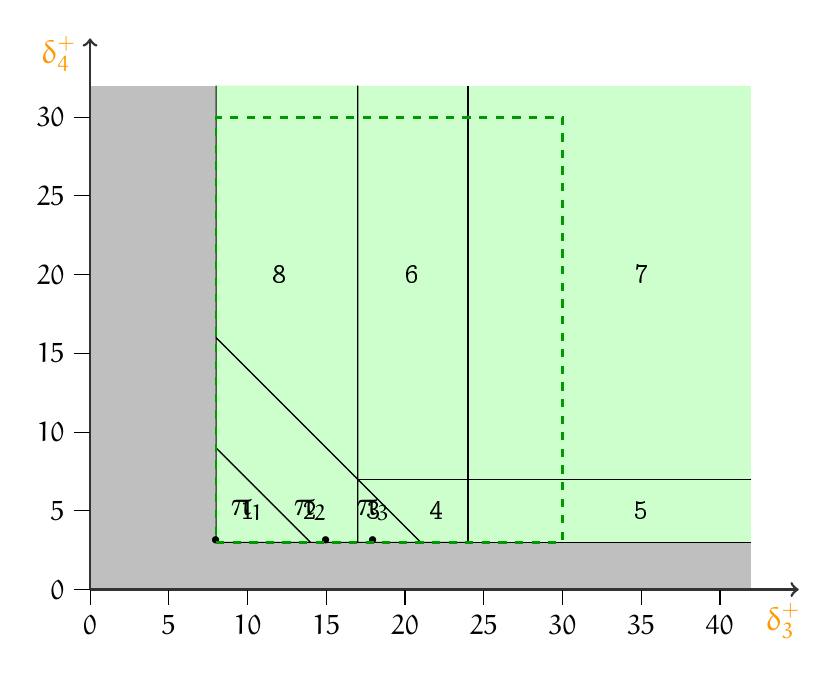
\begin{tikzpicture}[scale=.20]
	% STYLES
	\tikzstyle{axe} = [line width=1pt, ->, draw=black!80]
	\tikzstyle{v0} = [line width=1pt, draw=inputcolor, dashed]

	\tikzstyle{nomzone} = [draw=none, text=black]

	\tikzstyle{fondgris} = [fill=lightgray, draw=none]
	\tikzstyle{zonetmp} = [draw=black, fill=green!20!white]

	% FOND GRIS
	\draw[fondgris] (0, 0) rectangle (42, 32);

% 	% POINTS ENTIERS
% 	\foreach \x in {8, 9, ..., 30} % X
% 		\foreach \y in {3, 4, ..., 30}
% 			\node at (\x, \y) {\Large{$\textcolor{black!70}{\cdot}$}};
	
	% ZONE 1 : GOOD
	% dG3_u + dG4_u < 17   & dG4_u >= 3   & dG3_u >= 8
	\draw<3-> [zonetmp] (8, 3) -- (8, 9) -- (14, 3) -- cycle;
	\node<3->[nomzone] at (10, 5) {1};

	% ZONE 2 : GOOD
	% dG3_u + dG4_u < 24   & dG3_u >= 8   & dG3_u < 17   & dG3_u + dG4_u >= 17   & dG4_u >= 3
	\draw<5->[zonetmp] (8, 9) -- (8, 16) -- (17, 7) -- (17, 3) -- (14, 3) -- cycle;
	\node<5->[nomzone] at (14, 5) {2};

	% ZONE 3 : GOOD
	% & dG3_u >= 17   & dG3_u + dG4_u < 24   & dG4_u >= 3
	\draw<7->[zonetmp] (17, 7) -- (21, 3) -- (17, 3) -- cycle;
	\node<7->[nomzone] at (18, 5) {3};

	% ZONE 4 : BAD
	% dG4_u >= 3   & dG3_u < 24   & dG3_u + dG4_u >= 24   & dG4_u < 7
	\draw<8->[zonetmp] (17, 7) -- (24, 7) -- (24, 3) -- (21, 3) -- cycle;
	\node<8->[nomzone] at (22, 5) {4};

	% ZONE 5 : BAD
	% dG3_u >= 24   & dG4_u < 7   & dG4_u >= 3
	\draw<8->[zonetmp] (42, 3) -- (24, 3) -- (24, 7) -- (42, 7);
	\node<8->[nomzone] at (35, 5) {5};

	% ZONE 6 : BAD
	% dG4_u >= 7   & dG3_u >= 17   & dG3_u < 24
	\draw<8->[zonetmp] (24, 32) -- (24, 7) -- (17, 7) -- (17, 32);
	\node<8->[nomzone] at (20.5, 20) {6};

	% ZONE 7 : BAD
	%  dG3_u >= 24   & dG4_u >= 7
	\draw<8->[zonetmp, draw=none] (24, 7) -- (24, 32) -- (42, 32) -- (42, 7) -- cycle;
	\draw<8->[draw=black] (42, 7) -- (24, 7) -- (24, 32);
	\node<8->[nomzone] at (35, 20) {7};

	% ZONE 8 : BAD
	% dG3_u + dG4_u >= 24   & dG3_u >= 8   & dG3_u < 17
	\draw<8->[zonetmp] (17, 32) -- (17, 7) -- (8, 16) -- (8, 32);
	\node<8->[nomzone] at (12, 20) {8};
	
	% PI
	\node<2> at (8, 3) {\Huge{$\cdot$}};
	\node<2> at (10, 5) {\large{$\pi_1$}};
	\node<4> at (15, 3) {\Huge{$\cdot$}};
	\node<4> at (14, 5) {\large{$\pi_2$}};
	\node<6> at (18, 3) {\Huge{$\cdot$}};
	\node<6> at (18, 5) {\large{$\pi_3$}};
% 	\node<8> at (22, 3) {\Huge{$\cdot$}};
% 	\node<8> at (22, 5) {\large{$\pi_4$}};
% 	\node<10> at (25, 3) {\Huge{$\cdot$}};
% 	\node<10> at (25, 5) {\large{$\pi_5$}};
% 	\node<12> at (17, 8) {\Huge{$\cdot$}};
% 	\node<12> at (17, 10) {\large{$\pi_6$}};
% 	\node<14> at (25, 8) {\Huge{$\cdot$}};
% 	\node<14> at (25, 10) {\large{$\pi_7$}};
% 	\node<16> at (16, 9) {\Huge{$\cdot$}};
% 	\node<16> at (16, 11) {\large{$\pi_8$}};



	% AXES
	\path[axe] % X
		(0,0) -- ++ (45, 0);
	\path[axe] % Y
		(0,0) -- ++ (0, 35);
	\node at (44, -2) {\large $\coulparam{\delta_3^+}$};
	\node at (-2, 34) {\large $\coulparam{\delta_4^+}$};
	
	% VO
	\path[v0]
		(8, 3) -- ++ (22, 0) -- ++ (0, 27) -- ++ (-22, 0) -- cycle;
	
	% VALEURS
	\foreach \x in {0, 5, ..., 40} % X
		\draw (\x, 0) -- (\x, -1) node [below] {$\x$};
	\foreach \x in {0, 5, ..., 30} % Y
		\draw (0, \x) -- (-1, \x) node [left] {$\x$};
	
\end{tikzpicture}

}
%-%-%-%-%-%-%-%-%-%-%-%-%-%-%-%-%-%-%-%-%-%-%-%-%%



\end{frame}
%%%%%%%%%%%%%%%%%%%%%%%%%%%%%%%%%%%%%%%%%%%%%%%%%%%%%%%%%%%%%%%%%%%%%%%%%%%%%%%%%%



%%%%%%%%%%%%%%%%%%%%%%%%%%%%%%%%%%%%%%%%%%%%%%%%%%%%%%%%%%%%%%%%%%%%%%%%%%%%%%%%%%
\begin{frame}
\frametitle{Examples of Good and Bad Tiles for the Flip-flop}

\begin{itemize}
	\item \coulgood{Good} tile 3

{

\centering
\tiny

\begin{tikzpicture}[scale=0.38, ->, >=stealth', auto, node distance=1.00cm, thin]
\tikzstyle{state}=[circle, minimum size=12pt, draw=none, text=black, shade=ball, inner sep=1.5pt]

	\node[state, ball color=cv1] (Q0) at (0,4) {}; % {$q_0$};
	\node[state, ball color=cv2]         (Q1) at (3,4) {}; %{$q_1$};
	\node[state, ball color=cv3]         (Q2) at (6,4) {}; %{$q_2$};
	\node[state, ball color=cv4]         (Q3) at (9,4) {}; %{$q_3$};
	\node[state, ball color=cv5]         (Q4) at (12,2) {}; %{$q_4$};
	\node[state, ball color=cv6]         (Q5) at (12,4) {}; %{$q_5$};
% 	\node[state, fill=cv7]         (Q6) at (15,4) {$q_6$};
	\node[state, ball color=cv8]         (Q7) at (15,2) {}; %{$q_7$};
	\node[state, ball color=cv8]         (Q8) at (15,4) {}; %{$q_8$};
	\node[state, ball color=cv9]         (Q9) at (15,6) {}; %{$q_9$};
% 	\node[state, fill=cv10]        (Q10) at (18,0) {$q_{10}$};
	\node[state, ball color=cv11]        (Q11) at (18,2) {}; %{$q_{11}$};
% 	\node[state, fill=cv10]        (Q12) at (18,4) {$q_{12}$};
	\node[state, ball color=cv11]        (Q13) at (18,4) {}; %{$q_{13}$};
	\node[state, ball color=cv11]        (Q14) at (18,6) {}; %{$q_{14}$};
	\node[state, ball color=cv12]        (Q15) at (21,4) {}; %{$q_{15}$};
% 	\node[state, fill=cv12]        (Q16) at (21,4) {$q_{16}$};
	\node[state, ball color=cv12]        (Q17) at (21,2) {}; %{$q_{17}$};
% 	\node[state, fill=cv12]        (Q18) at (21,0) {$q_{18}$};
	\node[state, ball color=cv12]        (Q19) at (21,6) {}; %{$q_{19}$};

	\path
		(Q0) edge [double] node {$\coulact{D^\uparrow}$} (Q1)
		(Q1) edge [double] node {$\coulact{G_1^\downarrow}$} (Q2)
		(Q2) edge [double] node {$\coulact{\mathit{CK}^\uparrow}$} (Q3)
		(Q3) edge [double, below] node {$\coulact{D^\downarrow}$} (Q4)
		(Q3) edge [double] node {$\coulact{G_3^\downarrow}$} (Q5)
		(Q4) edge [double] node {$\coulact{G_3^\downarrow}$} (Q7)
% 		(Q4) edge [double] node {$\coulact{\mathit{CK}^\downarrow$} (Q6)
		(Q5) edge [double] node {$\coulact{D^\downarrow}$} (Q8)
		(Q5) edge [double] node {$\coulact{Q^\uparrow}$} (Q9)
% 		(Q7) edge [double, below left] node {$\coulact{\mathit{CK}^\downarrow$} (Q10)
		(Q7) edge [double] node {$\coulact{Q^\uparrow}$} (Q11)
% 		(Q8) edge [double, below] node {$\coulact{\mathit{CK}^\downarrow$} (Q12)
		(Q8) edge [double] node {$\coulact{Q^\uparrow}$} (Q13)
		(Q9) edge [double] node {$\coulact{D^\downarrow}$} (Q14)
% 		(Q10) edge [double] node {$\coulact{Q^\uparrow$} (Q18)
		(Q11) edge [double] node {$\coulact{\mathit{CK}^\downarrow}$} (Q17)
% 		(Q12) edge [double] node {$\coulact{Q^\uparrow$} (Q16)
		(Q13) edge [double] node {$\coulact{\mathit{CK}^\downarrow}$} (Q15)
		(Q14) edge [double] node {$\coulact{\mathit{CK}^\downarrow}$} (Q19)
		;

\end{tikzpicture}
%%-%-%-%-%-%-%-%-%-%-%-%-%-%-%-%-%-%-%-%-%-%-%-%-%

}

	\bigskip
	\bigskip

	\item \coulbad{Bad} tile 7

{

\centering
\tiny

\begin{tikzpicture}[scale=0.38, ->, >=stealth', auto, node distance=1.00cm, thin]
\tikzstyle{state}=[circle, minimum size=12pt, draw=none, text=black, shade=ball, inner sep=1.5pt]

	\node[state, ball color=cv1] (Q0) at (0,4) {}; %{$q_0$};
	\node[state, ball color=cv2]         (Q1) at (3,4) {}; %{$q_1$};
	\node[state, ball color=cv3]         (Q2) at (6,4) {}; %{$q_2$};
	\node[state, ball color=cv4]         (Q3) at (9,4) {}; %{$q_3$};
	\node[state, ball color=cv5]         (Q4) at (12,4) {}; %{$q_4$};
	\node[state, ball color=cv6]         (Q5) at (12,6) {}; %{$q_5$};
	\node[state, ball color=cv7]         (Q6) at (15,4) {}; %{$q_6$};
	\node[state, ball color=cv8]         (Q7) at (15,2) {}; %{$q_7$};
	\node[state, ball color=cv8]         (Q8) at (15,6) {}; %{$q_8$};
	\node[state, ball color=cv9]         (Q9) at (15,8) {}; %{$q_9$};
	\node[state, ball color=cv10]        (Q10) at (18,0) {}; %{$q_{10}$};
	\node[state, ball color=cv11]        (Q11) at (18,2) {}; %{$q_{11}$};
	\node[state, ball color=cv10]        (Q12) at (18,4) {}; %{$q_{12}$};
	\node[state, ball color=cv11]        (Q13) at (18,6) {}; %{$q_{13}$};
	\node[state, ball color=cv11]        (Q14) at (18,8) {}; %{$q_{14}$};
	\node[state, ball color=cv12]        (Q15) at (21,6) {}; %{$q_{15}$};
	\node[state, ball color=cv12]        (Q16) at (21,4) {}; %{$q_{16}$};
	\node[state, ball color=cv12]        (Q17) at (21,2) {}; %{$q_{17}$};
	\node[state, ball color=cv12]        (Q18) at (21,0) {}; %{$q_{18}$};
	\node[state, ball color=cv12]        (Q19) at (21,8) {}; %{$q_{19}$};

	\path
		(Q0) edge [double] node {$\coulact{D^\uparrow}$} (Q1)
		(Q1) edge [double] node {$\coulact{G_1^\downarrow}$} (Q2)
		(Q2) edge [double] node {$\coulact{\mathit{CK}^\uparrow}$} (Q3)
		(Q3) edge [double, below] node {$\coulact{D^\downarrow}$} (Q4)
		(Q3) edge [double] node {$\coulact{G_3^\downarrow}$} (Q5)
		(Q4) edge [double, below left] node {$\coulact{G_3^\downarrow}$} (Q7)
		(Q4) edge [double] node {$\coulact{\mathit{CK}^\downarrow}$} (Q6)
		(Q5) edge [double] node {$\coulact{D^\downarrow}$} (Q8)
		(Q5) edge [double] node {$\coulact{Q^\uparrow}$} (Q9)
		(Q7) edge [double, below left] node {$\coulact{\mathit{CK}^\downarrow}$} (Q10)
		(Q7) edge [double] node {$\coulact{Q^\uparrow}$} (Q11)
		(Q8) edge [double, below left] node {$\coulact{\mathit{CK}^\downarrow}$} (Q12)
		(Q8) edge [double] node {$\coulact{Q^\uparrow}$} (Q13)
		(Q9) edge [double] node {$\coulact{D^\downarrow}$} (Q14)
		(Q10) edge [double] node {$\coulact{Q^\uparrow}$} (Q18)
		(Q11) edge [double] node {$\coulact{\mathit{CK}^\downarrow}$} (Q17)
		(Q12) edge [double] node {$\coulact{Q^\uparrow}$} (Q16)
		(Q13) edge [double] node {$\coulact{\mathit{CK}^\downarrow}$} (Q15)
		(Q14) edge [double] node {$\coulact{\mathit{CK}^\downarrow}$} (Q19)
		;

\end{tikzpicture}
%%-%-%-%-%-%-%-%-%-%-%-%-%-%-%-%-%-%-%-%-%-%-%-%-%

}

\end{itemize}

\end{frame}
%%%%%%%%%%%%%%%%%%%%%%%%%%%%%%%%%%%%%%%%%%%%%%%%%%%%%%%%%%%%%%%%%%%%%%%%%%%%%%%%%%





%%%%%%%%%%%%%%%%%%%%%%%%%%%%%%%%%%%%%%%%%%%%%%%%%%%%%%%%%%%%%%%%%%%%%%%%%%%%%%%%%%
\begin{frame}
\frametitle{Behavioral Cartography of the Flip-flop: Partition }


%-%-%-%-%-%-%-%-%-%-%-%-%-%-%-%-%-%-%-%-%-%-%-%-%%
{
\centering
\scriptsize

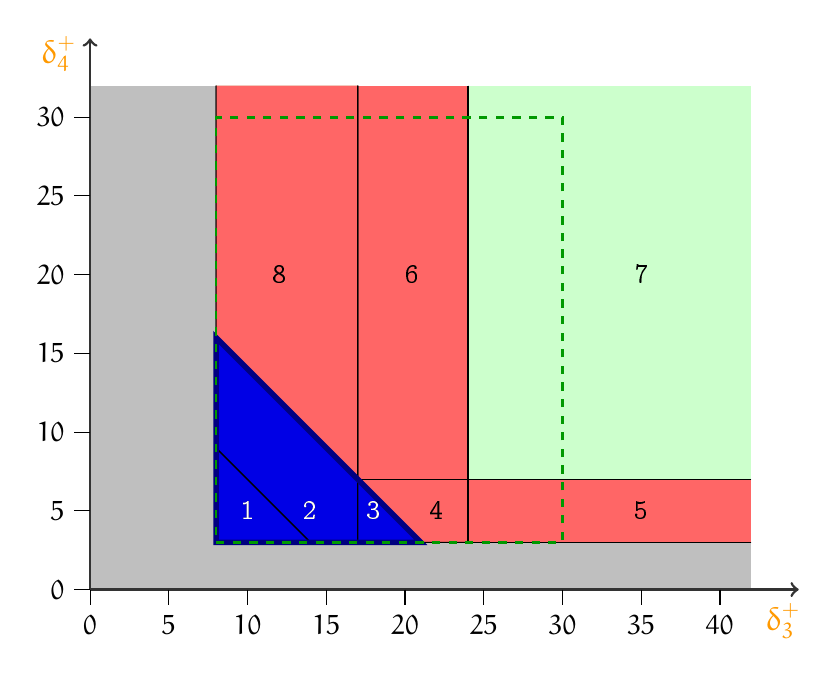
\begin{tikzpicture}[scale=.20]
	% STYLES
	\tikzstyle{axe} = [line width=1pt, ->, draw=black!80]
	\tikzstyle{goodzone} = [line width=2pt, draw=blue!50!black]
	\tikzstyle{v0} = [line width=1pt, draw=inputcolor, dashed]

	\tikzstyle{nomzonegood} = [draw=none, text=white]
	\tikzstyle{nomzonebad} = [draw=none, text=black]

	\tikzstyle{fondgris} = [fill=lightgray, draw=none]
	\tikzstyle{zonebad} = [draw=black, fill=red!60!white]
	\tikzstyle{zonegood} = [draw=black, fill=blue!90!black]
	\tikzstyle{zonetmp} = [draw=black, fill=green!20!white]

	% AXES
	\draw[fondgris] (0, 0) rectangle (42, 32);

	% ZONE 1 : GOOD
	% dG3_u + dG4_u < 17   & dG4_u >= 3   & dG3_u >= 8
	\draw<1> [zonetmp] (8, 3) -- (8, 9) -- (14, 3) -- cycle;
	\draw<2->[zonegood] (8, 3) -- (8, 9) -- (14, 3) -- cycle;
	\node<1>[nomzonebad] at (10, 5) {1};
	\node<2->[nomzonegood] at (10, 5) {1};

	% ZONE 2 : GOOD
	% dG3_u + dG4_u < 24   & dG3_u >= 8   & dG3_u < 17   & dG3_u + dG4_u >= 17   & dG4_u >= 3
	\draw<1>[zonetmp] (8, 9) -- (8, 16) -- (17, 7) -- (17, 3) -- (14, 3) -- cycle;
	\draw<2->[zonegood] (8, 9) -- (8, 16) -- (17, 7) -- (17, 3) -- (14, 3) -- cycle;
	\node<1>[nomzonebad] at (14, 5) {2};
	\node<2->[nomzonegood] at (14, 5) {2};

	% ZONE 3 : GOOD
	% & dG3_u >= 17   & dG3_u + dG4_u < 24   & dG4_u >= 3
	\draw<1>[zonetmp] (17, 7) -- (21, 3) -- (17, 3) -- cycle;
	\draw<2->[zonegood] (17, 7) -- (21, 3) -- (17, 3) -- cycle;
	\node<1>[nomzonebad] at (18, 5) {3};
	\node<2->[nomzonegood] at (18, 5) {3};

	% ZONE 4 : BAD
	% dG4_u >= 3   & dG3_u < 24   & dG3_u + dG4_u >= 24   & dG4_u < 7
	\draw<1>[zonetmp] (17, 7) -- (24, 7) -- (24, 3) -- (21, 3) -- cycle;
	\draw<2->[zonebad] (17, 7) -- (24, 7) -- (24, 3) -- (21, 3) -- cycle;
	\node<1->[nomzonebad] at (22, 5) {4};

	% ZONE 5 : BAD
	% dG3_u >= 24   & dG4_u < 7   & dG4_u >= 3
	\draw<1>[zonetmp] (42, 3) -- (24, 3) -- (24, 7) -- (42, 7);
	\draw<2->[zonebad] (42, 3) -- (24, 3) -- (24, 7) -- (42, 7);
	\node<1->[nomzonebad] at (35, 5) {5};

	% ZONE 6 : BAD
	% dG4_u >= 7   & dG3_u >= 17   & dG3_u < 24
	\draw<1>[zonetmp] (24, 32) -- (24, 7) -- (17, 7) -- (17, 32);
	\draw<2->[zonebad] (24, 32) -- (24, 7) -- (17, 7) -- (17, 32);
	\node<1->[nomzonebad] at (20.5, 20) {6};

	% ZONE 7 : BAD
	%  dG3_u >= 24   & dG4_u >= 7
	\draw<2->[zonebad, draw=none] (24, 7) -- (24, 32) -- (42, 32) -- (42, 7) -- cycle;
	\draw<1>[zonetmp, draw=none] (24, 7) -- (24, 32) -- (42, 32) -- (42, 7) -- cycle;
	\draw<1->[draw=black] (42, 7) -- (24, 7) -- (24, 32);
	\node<1->[nomzonebad] at (35, 20) {7};

	% ZONE 8 : BAD
	% dG3_u + dG4_u >= 24   & dG3_u >= 8   & dG3_u < 17
	\draw<1>[zonetmp] (17, 32) -- (17, 7) -- (8, 16) -- (8, 32);
	\draw<2->[zonebad] (17, 32) -- (17, 7) -- (8, 16) -- (8, 32);
	\node<1->[nomzonebad] at (12, 20) {8};


	% GOOD ZONE
	\draw<2->[goodzone]
		(8, 3) -- (8, 16) -- (21, 3) -- cycle;

	% AXES
	\path[axe] % X
		(0,0) -- ++ (45, 0);
	\path[axe] % Y
		(0,0) -- ++ (0, 35);
	\node at (44, -2) {\large $\coulparam{\delta_3^+}$};
	\node at (-2, 34) {\large $\coulparam{\delta_4^+}$};
	
	% VO
	\path[v0]
		(8, 3) -- ++ (22, 0) -- ++ (0, 27) -- ++ (-22, 0) -- cycle;
	
	% VALEURS
	\foreach \x in {0, 5, ..., 40} % X
		\draw (\x, 0) -- (\x, -1) node [below] {$\x$};
	\foreach \x in {0, 5, ..., 30} % Y
		\draw (0, \x) -- (-1, \x) node [left] {$\x$};
	
\end{tikzpicture}

}
%-%-%-%-%-%-%-%-%-%-%-%-%-%-%-%-%-%-%-%-%-%-%-%-%%



\end{frame}
%%%%%%%%%%%%%%%%%%%%%%%%%%%%%%%%%%%%%%%%%%%%%%%%%%%%%%%%%%%%%%%%%%%%%%%%%%%%%%%%%%



%%%%%%%%%%%%%%%%%%%%%%%%%%%%%%%%%%%%%%%%%%%%%%%%%%%%%%%%%%%%%%%%%%%%%%%%%%%%%%%%%%
\begin{frame}
\frametitle{Behavioral Cartography of the Flip-flop: Remarks}

\begin{itemize}
	\item Remarks on the cartography

	\begin{itemize}
		\item For this example, \couleur{all the real-valued part} of the parametric space within and outside $\Vo$ is covered
	\end{itemize}
	
	\bigskip

	\item The \couleur{set of good tiles} (in blue) corresponds to the \couleur{maximal set} of good values for $\delta_3^+$ and $\delta_4^+$
	\begin{itemize}
		\item $ \delta_3^+ + \delta_4^+ \leq 24 \ \ \land \ \ \delta_3^+ \geq 8  \ \ \land \ \ \delta_4^+ \geq 3 $
	\end{itemize}

\end{itemize}

\end{frame}
%%%%%%%%%%%%%%%%%%%%%%%%%%%%%%%%%%%%%%%%%%%%%%%%%%%%%%%%%%%%%%%%%%%%%%%%%%%%%%%%%%





%%%%%%%%%%%%%%%%%%%%%%%%%%%%%%%%%%%%%%%%%%%%%%%%%%%%%%%%%%%%%%%%%%%%%%%%%%%%%%%%%%
%%%%%%%%%%%%%%%%%%%%%%%%%%%%%%%%%%%%%%%%%%%%%%%%%%%%%%%%%%%%%%%%%%%%%%%%%%%%%%%%%%
\section{Implementation and Applications}
%%%%%%%%%%%%%%%%%%%%%%%%%%%%%%%%%%%%%%%%%%%%%%%%%%%%%%%%%%%%%%%%%%%%%%%%%%%%%%%%%%
%%%%%%%%%%%%%%%%%%%%%%%%%%%%%%%%%%%%%%%%%%%%%%%%%%%%%%%%%%%%%%%%%%%%%%%%%%%%%%%%%%



%%%%%%%%%%%%%%%%%%%%%%%%%%%%%%%%%%%%%%%%%%%%%%%%%%%%%%%%%%%%%%%%%%%%%%%%%%%%%%%%%%%
% Plan
\begin{frame}
	\frametitle{\plan{}}
	\tableofcontents[currentsection, hideallsubsections]
\end{frame}
%%%%%%%%%%%%%%%%%%%%%%%%%%%%%%%%%%%%%%%%%%%%%%%%%%%%%%%%%%%%%%%%%%%%%%%%%%%%%%%%%%


%%%%%%%%%%%%%%%%%%%%%%%%%%%%%%%%%%%%%%%%%%%%%%%%%%%%%%%%%%%%%%%%%%%%%%%%%%%%%%%%%
\subsection{Implementation}
%%%%%%%%%%%%%%%%%%%%%%%%%%%%%%%%%%%%%%%%%%%%%%%%%%%%%%%%%%%%%%%%%%%%%%%%%%%%%%%%%


%%%%%%%%%%%%%%%%%%%%%%%%%%%%%%%%%%%%%%%%%%%%%%%%%%%%%%%%%%%%%%%%%%%%%%%%%%%%%%%%%%
\begin{frame}
\frametitle{Implementation}

\begin{itemize}
	\item \couleur{\imitator{}} 2.5 \refer{afks12}

	\begin{itemize}
		\item \imitator{}: ``\couleur{I}nverse \couleur{M}ethod for \couleur{I}nferring \couleur{T}ime \couleur{A}bstrac\couleur{T} Behavi\couleur{OR}''
		\item 10\,000 lines of code
		\item Program written in \couleur{\ocaml{}}
		\item Makes use of the \couleur{PPL} library for handling polyhedra % \refer{bhz08}
	\end{itemize}

	\medskip

	\item Main contributors

	\begin{itemize}
		\item \'E. Andr\'e, L. Fribourg, U. K\"uhne, R. Soulat
	\end{itemize}

	\medskip

	\item Available on the Web

	\begin{itemize}
		\item \couleur{\url{http://www.lsv.ens-cachan.fr/Software/imitator/}}
	\end{itemize}

	\pause
	
	\medskip

	\item And now part of CosyVerif!


\end{itemize}

\end{frame}
%%%%%%%%%%%%%%%%%%%%%%%%%%%%%%%%%%%%%%%%%%%%%%%%%%%%%%%%%%%%%%%%%%%%%%%%%%%%%%%%%%



%%%%%%%%%%%%%%%%%%%%%%%%%%%%%%%%%%%%%%%%%%%%%%%%%%%%%%%%%%%%%%%%%%%%%%%%%%%%%%%%%
\subsection{Applications}
%%%%%%%%%%%%%%%%%%%%%%%%%%%%%%%%%%%%%%%%%%%%%%%%%%%%%%%%%%%%%%%%%%%%%%%%%%%%%%%%%

%%%%%%%%%%%%%%%%%%%%%%%%%%%%%%%%%%%%%%%%%%%%%%%%%%%%%%%%%%%%%%%%%%%%%%%%%%%%%%%%%%
\begin{frame}
\frametitle{Case Studies and Main Projects}

\begin{itemize}
	\item Applications

	\begin{itemize}
		\item Asynchronous circuits
		\item Communication protocols
		\item Scheduling problems
	\end{itemize}

	\bigskip

	\item Industrial projects

	\begin{itemize}
		\item ANR \couleur{Valmem} (with ST-Microelectronics) : 2007--2010 \refer{ACEF09}
		
		\medskip
		
		\item Farman \couleur{ROSCOV} (with EADS Astrium Space Transportation) : 2012--2013 \refer{FLMS12}
	\end{itemize}


\end{itemize}

\end{frame}
%%%%%%%%%%%%%%%%%%%%%%%%%%%%%%%%%%%%%%%%%%%%%%%%%%%%%%%%%%%%%%%%%%%%%%%%%%%%%%%%%%





%%%%%%%%%%%%%%%%%%%%%%%%%%%%%%%%%%%%%%%%%%%%%%%%%%%%%%%%%%%%%%%%%%%%%%%%%%%%%%%%%%
\begin{frame}
\frametitle{The \spsmall{} Memory}

\only<1>
{
\centering
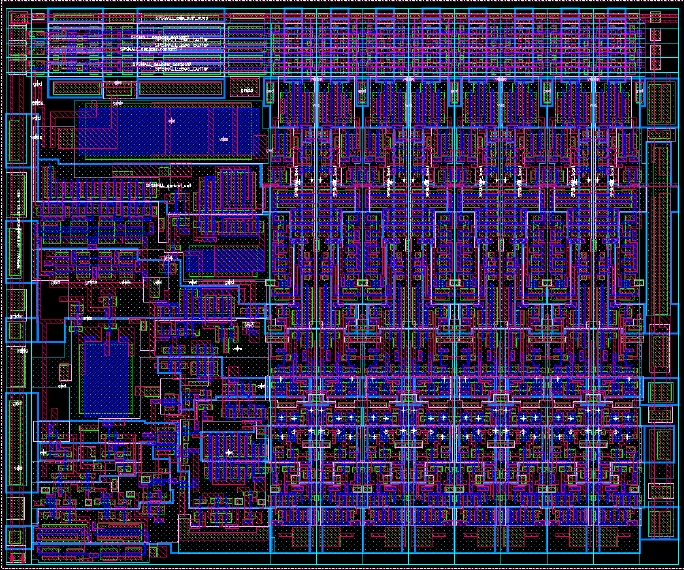
\includegraphics[width=0.015\textwidth]{spsmall_moche.jpg}

}

\only<2>
{
\centering
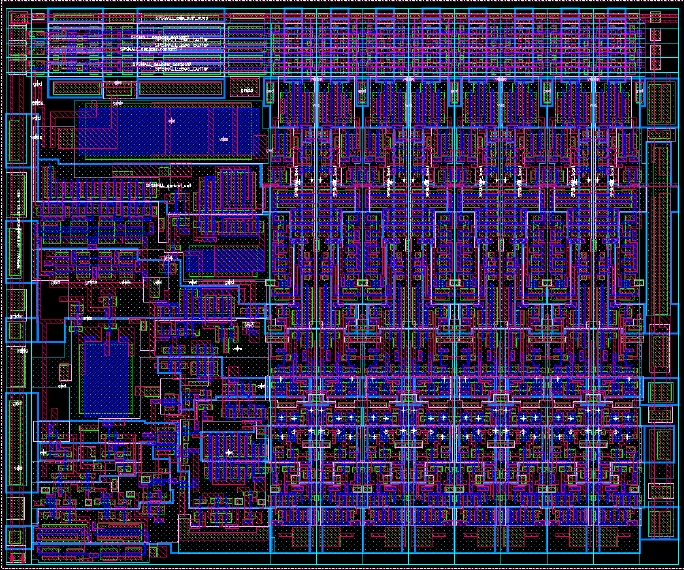
\includegraphics[width=0.75\textwidth]{spsmall_moche.jpg}

}

\end{frame}
%%%%%%%%%%%%%%%%%%%%%%%%%%%%%%%%%%%%%%%%%%%%%%%%%%%%%%%%%%%%%%%%%%%%%%%%%%%%%%%%%%



%%%%%%%%%%%%%%%%%%%%%%%%%%%%%%%%%%%%%%%%%%%%%%%%%%%%%%%%%%%%%%%%%%%%%%%%%%%%%%%%%%
\begin{frame}
\frametitle{The \spsmall{} Memory: Minimization of Timings}

\begin{itemize}
	\item Partition into good and bad tiles
	\begin{itemize}
		\item Using the property of good behavior specified by the datasheet
	\end{itemize}
	
	\medskip
	
	%-%-%-%-%-%-%-%-%-%-%-%-%-%-%-%-%-%-%-%-%-%-%-%-%%
	{
	\centering
	\tiny

	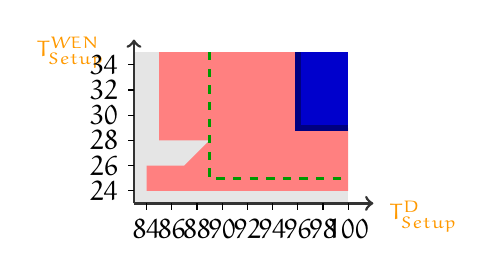
\begin{tikzpicture}[scale=0.16]
		% STYLES
		\tikzstyle{axe} = [line width=1pt, ->, draw=black!80]
		\tikzstyle{goodzone} = [line width=2pt, draw=blue!50!black]
		\tikzstyle{v0} = [line width=1pt, draw=inputcolor, dashed]

		\tikzstyle{fondgris} = [fill=grispale, draw=none]
		\tikzstyle{zone} = [draw=none]

		% FOND
	% 	\draw[fondgris] (89, 98) rectangle (12, 8);
		\path[fondgris]
			(83, 23) -- (100, 23) -- (100, 35) -- (83, 35) -- cycle;

		% ZONE 1 : BAD
% 		\draw[zone, fill=red!50!white] (85, 34) -- (85, 28) -- (89, 28) -- (87, 26) -- (84, 26) -- (84, 24) -- (99, 24) -- (99, 29) -- (96, 29) -- (96, 34) -- cycle;
		\draw[zone, fill=red!50!white] (85, 35) -- (85, 28) -- (89, 28) -- (87, 26) -- (84, 26) -- (84, 24) -- (100, 24) -- (100, 29) -- (96, 29) -- (96, 35) -- cycle;

		% ZONE 2 : GOOD
% 		\draw[zone, fill=blue!80!black] (96, 29) -- (99, 29) -- (99, 33) -- (98, 33) -- (99, 34) -- (96, 34) -- cycle;
		\draw[zone, fill=blue!80!black] (96, 35) -- (100, 35) -- (100, 29) -- (96, 29) -- cycle;
		

		% GOOD D'APRES ABDEL
	%     t_setup_d_0 = 96 .. 108,
	%     t_setup_a_0 = 31 .. 58,
	%     t_setup_wen = 29 .. 48,

		% GOOD ZONE
% 		\draw[goodzone]
% 			(96, 29) -- (99, 29) -- (99, 33) -- (98, 33) -- (99, 34) -- (96, 34) -- cycle;
		\draw[goodzone]
			(96, 35) -- (96, 29) -- (100, 29);


		% AXES
		\path[axe] % X
			(83, 23) -- (102, 23);
		\path[axe] % Y
			(83, 23) -- (83, 36);
		\node at (106, 22) {\footnotesize $\tSetupD$}; % X
		\node at (78, 35) {\footnotesize $\tSetupWen$}; % Y
		
		% VO : \tSetupD \in [89; 98]  \ \ \land \ \ \tSetupWen \in [25; 34]
		\path[v0]
% 			(89, 25) -- (89, 34) -- (98, 34) -- (98, 25) -- cycle;
			(89, 35) -- (89, 25) -- (100, 25);
		
		% VALEURS
		\foreach \x in {84, 86, ..., 100} % X
			\draw (\x, 23) -- (\x, 22.5) node [below] {$\x$};
		\foreach \x in {24, 26, ..., 34} % Y
			\draw (83, \x) -- (82.5, \x) node [left] {$\x$};
		
	\end{tikzpicture}
	
	}
	%-%-%-%-%-%-%-%-%-%-%-%-%-%-%-%-%-%-%-%-%-%-%-%-%%

	\smallskip

	\item<2-> Minimization of timing delays
	\begin{itemize}
		\item $\tSetupD = 108$ \only<3->{$\leadsto \couleur{96}$ (decrease of $\couleur{11.1\,\%}$)}
		\item $\tSetupWen = 48$ \only<3->{$\leadsto \couleur{29}$ (decrease of $\couleur{39.6\,\%}$)}
	\end{itemize}

	\medskip

	\item<4-> Practical interest: allows to work in a \couleur{faster environment}
	\begin{itemize}
		\item \couleur{Optimization} of the datasheet
		\item \couleur{Financial interest}
	\end{itemize}


\end{itemize}

\end{frame}
%%%%%%%%%%%%%%%%%%%%%%%%%%%%%%%%%%%%%%%%%%%%%%%%%%%%%%%%%%%%%%%%%%%%%%%%%%%%%%%%%%





%%%%%%%%%%%%%%%%%%%%%%%%%%%%%%%%%%%%%%%%%%%%%%%%%%%%%%%%%%%%%%%%%%%%%%%%%%%%%%%%%%
\begin{frame}
\frametitle{The ROSCOV Project with Astrium}

\begin{center}
	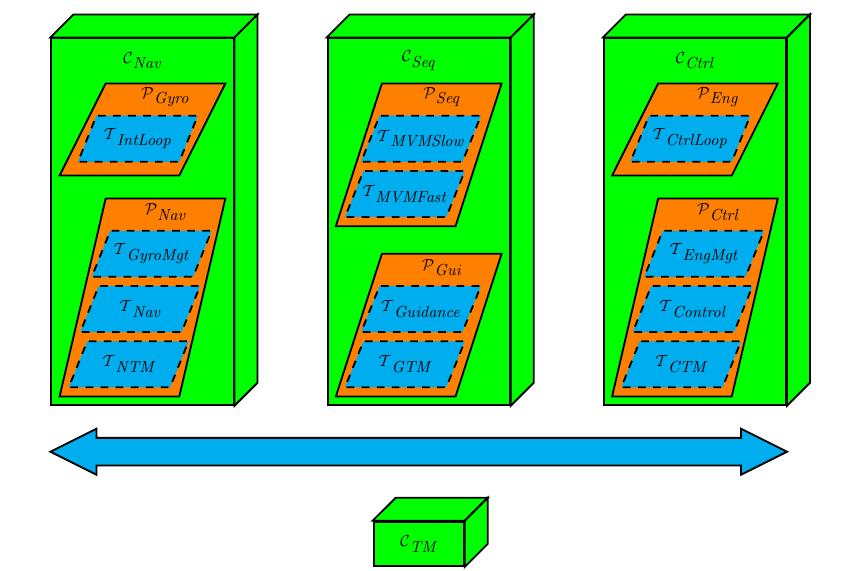
\includegraphics[width=0.7\textwidth]{astrium_ex.jpg}
\end{center}


Prospective architecture for the flight control system of the next generation of autonomous transfer vehicles (ATV)

\end{frame}
%%%%%%%%%%%%%%%%%%%%%%%%%%%%%%%%%%%%%%%%%%%%%%%%%%%%%%%%%%%%%%%%%%%%%%%%%%%%%%%%%%



%%%%%%%%%%%%%%%%%%%%%%%%%%%%%%%%%%%%%%%%%%%%%%%%%%%%%%%%%%%%%%%%%%%%%%%%%%%%%%%%%%
\begin{frame}
\frametitle{The ROSCOV Project: Robust Scheduling}

Robustness analysis for scheduling problems

\medskip

\begin{center}
	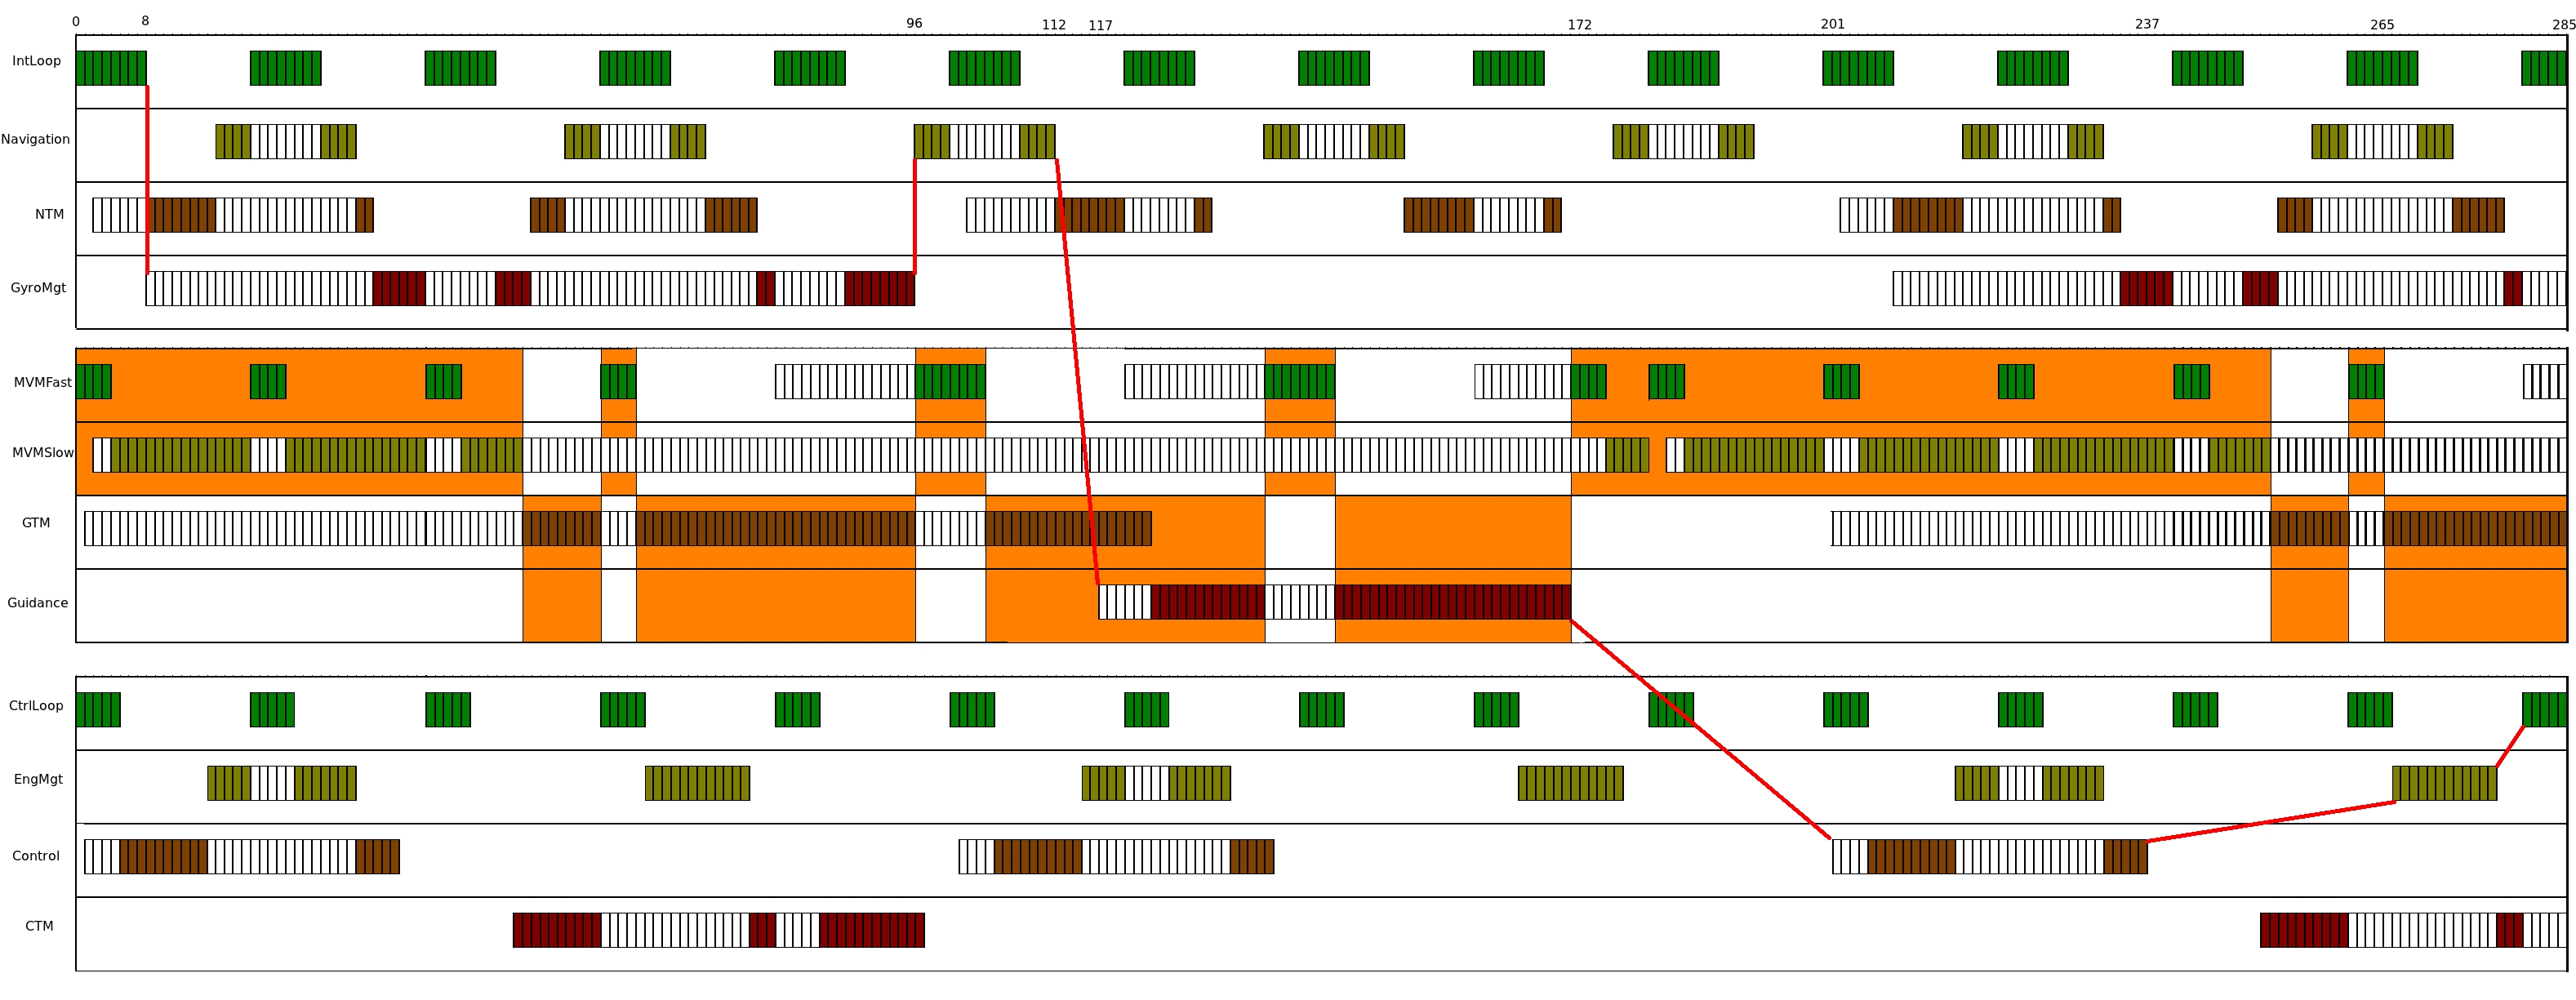
\includegraphics[width=0.8\textwidth]{chrono_test.jpg}
\end{center}
	
% \medskip

\begin{itemize}
% 	\item 
% 
% 	\bigskip
	
	\item Use of \imitator{} to synthesize a constraint \\
		$\leadsto$ Guarantee that the scheduling \couleur{meets the deadline}
\end{itemize}



\end{frame}
%%%%%%%%%%%%%%%%%%%%%%%%%%%%%%%%%%%%%%%%%%%%%%%%%%%%%%%%%%%%%%%%%%%%%%%%%%%%%%%%%%








%%%%%%%%%%%%%%%%%%%%%%%%%%%%%%%%%%%%%%%%%%%%%%%%%%%%%%%%%%%%%%%%%%%%%%%%%%%%%%%%%%
\end{document}
%%%%%%%%%%%%%%%%%%%%%%%%%%%%%%%%%%%%%%%%%%%%%%%%%%%%%%%%%%%%%%%%%%%%%%%%%%%%%%%%%%
%%%%%%%%%%%%%%%%%%%%%%%%%%%%%%%%%%%%%%%%%%%%%%%%%%%%%%%%%%%%%%%%%%%%%%%%%%%%%%%%%%
